\documentclass[12 pt, onesided]{book}

% Vertical bars
\usepackage{amsmath}

% Handle characters beyond ASCII nicely
\usepackage[utf8]{inputenc}

% Make the References section show up in the table of contents
\usepackage[nottoc, numbib]{tocbibind}

% Let us cite the bibliography entries
\usepackage{cite}

% Time to add images
\usepackage{graphicx}
\graphicspath{{Img/}}

% Links please!
\usepackage{hyperref}

% Format the links
\hypersetup{
    pdfborder = {0 0 0},    % Remove the ugly border
    colorlinks = true,      % Let there be color
    citecolor = black,      % Make citations appear normal (i.e black)
    linkcolor = black,      % The same for links (i.e table of contents)
    urlcolor = cyan         % Color the web links. (cyan is fancy for blueish...)
}

% Code listings. Taken from: https://www.overleaf.com/learn/latex/Code_listing
\usepackage{listings, lstautogobble}
\usepackage{xcolor}

\definecolor{codegreen}{rgb}{0,0.6,0}
\definecolor{codegray}{rgb}{0.5,0.5,0.5}
\definecolor{codepurple}{rgb}{0.58,0,0.82}
\definecolor{backcolour}{rgb}{0.95,0.95,0.92}

\lstdefinestyle{mystyle}{
    % backgroundcolor = \color{backcolour},
    commentstyle = \color{codegreen},
    keywordstyle = \color{magenta},
    numberstyle = \tiny\color{codegray},
    stringstyle = \color{codepurple},
    basicstyle = \ttfamily\footnotesize,
    breakatwhitespace = false,
    breaklines = true,
    captionpos = b,
    keepspaces = true,
    numbers = left,
    numbersep = 5pt,
    showspaces = false,
    showstringspaces = false,
    showtabs = false,
    tabsize = 2,
    autogobble = true
}

\lstset{style = mystyle}

% Use minted for code highlighting. Minted doc -> http://mirror.ox.ac.uk/sites/ctan.org/macros/latex/contrib/minted/minted.pdf
\usepackage{minted}

% Define new environments with settings and all. Use it with \begin{pycode}\end{pycode}
\newminted{py}{
    frame = lines,
    style = emacs,
    linenos
}

% Style input files. Use it with \pyfile{path/from/Book/directory/foo.py}
\newmintedfile{py}{
    frame = lines,
    style = emacs,
    linenos
}

% Modify the margins
% \usepackage{geometry}
% \geometry{
%     a4paper,
%     left = 18mm,
%     right = 18mm,
%     top = 14mm,
% }

% Enable fixed-width centered columns
% \usepackage{array}
% \newcolumntype{P}[1]{>{\centering\arraybackslash}p{#1}}

% Insert space between paragraphs
\newcommand{\newpar} {
    \vskip 0.5cm
}

% Remove the title page's number
\usepackage{titling}

\title{Think about something witty}
\author{Pablo \\ \\ \textbf{\texttt{TFG}} \\ \\ \textbf{Universidad de Alcalá}}
\date{}

\begin{document}
    % Use roman numerals until we issue \mainmatter
    \frontmatter

    % Avoid printing page numbers until we
        % issue \pagestyle{headings}
    \pagestyle{empty}

    % Visual Cover
        
\includepdf[pages = 1]{Content/Covers.pdf}

    % Textual Cover
        \newgeometry{top = 2cm, left = 3cm, right = 2cm}
            \begin{center}
    {\Huge UNIVERSIDAD DE ALCALÁ}\\
    \vspace{0.5cm}
    {\huge Escuela Politécnica Superior}\\
    \vspace{1.5cm}
    {\Large \textbf{Grado en Ingeniería Telemática}}\\
    \vspace{3cm}
    {\Large \textbf{Developing a Network Virtualization Framework for Testing Network Resilience Techniques}}\\
    \vspace{1.5cm}
    {\large Author: \textit{Pablo Collado Soto}}\\
    \vspace{2.5mm}
    {\large Tutor: \textit{Iván Marsá Maestre}}\\
    \vspace{2cm}
\end{center}

\begin{flushleft}
    {\large \textbf{Comittee:}}\\
    \vspace{1cm}
    {\large \hspace{2cm} \textbf{President:} \hspace{9mm} \textit{José Manuel Giménez Guzmán}}\\
    \vspace{0.5cm}
    {\large \hspace{2cm} \textbf{First Member:} \textit{Luis de la Cruz Piris}}\\
    \vspace{0.5cm}
    {\large \hspace{2cm} \textbf{Tutor:} \hspace{18mm} \textit{Iván Marsá Maestre}}\\
    \vspace{6cm}
\end{flushleft}

\begin{center}
    $23$ June $2021$
\end{center}

\clearpage

        \restoregeometry

    % Empty Page
        \newpage
            \null
        \newpage

    % ACKs
        \newgeometry{top = 2cm}
            \chapter*{ACKs}
    % Given how the \chpater{} command is defined this line is explicitly needed
        % despite having set \pagestyle{empty} before...
        % See https://tex.stackexchange.com/questions/19738/why-doesnt-pagestyleempty-work-on-the-first-page-of-a-chapter
    \thispagestyle{empty}

    This project marks the end of a key step in my academic and personal lives. I could not have tackled such a task without the help I have been gifted by many more individuals than I can really account for. However, I will try to do my best to thank as many as I possibly can.\\

    I would like to thank my parents. Even though when asked about what I do they just say ``there are a bunch of weird letters moving on screen'' they have always been there for me along the way. Figures such as my uncle, \textit{Chema Luzón} and my grandmother, \textit{Josefina Álvarez} have also played a crucial role in my academic progression: they showed me, by example, the meaning and value of pure, raw knowledge.\\

    If there is something I know for sure is I would not have made it here if it were not for all the teachers I have had, both good and bad. The best teachers have not only transmitted the technical knowledge I have made use of time and time again, but they also taught me how to think and how to appreciate knowledge for what it is. Teachers such as \textit{Francisco José Álvarez}, \textit{Antonio García}, \textit{José Manuel Giménez}, \textit{Javier Macías}, \textit{Iván Marsá}, \textit{Isaías Martínez}, \textit{Manuel Moreno}, \textit{Rosalino Pulido} and \textit{Elisa Rojas} have given me more than they know.\\

    It is quite difficult to understate the role my friends and loved ones have played in the years leading to this moment. Classmates such as \textit{David Gaupp} and \textit{Cristian Morales}, long time friends such as \textit{Carlos Corbella}, \textit{Gonzalo Martínez} and \textit{Alberto Río} and my partner, \textit{Alicia}, have made the road a thrill.\\

    I would finally like to personally thank \textit{David Carrascal}. He has not only provided direct help on this project (including this report) and many others, but he has also been one of the people we have shared the most with. Despite meeting towards the end of the degree he has proven to be, time and time again, the most knowledgeable person I know. His drive and passion for what he does has motivated me to try and improve every single day. Nonetheless and, more importantly, he has also been a great friend who makes you feel at ease with no matter what.\\

    I am certain somebody is being left out. One of the best things of knowing nothing is that everybody can teach and show you something. Given there is not enough paper in the world to write down every single person's name I only ask that nobody feels ignored: everybody I have ever met has played a role, either big or small, in me being here. I cannot say anything but \textit{thank you}.\\

        \restoregeometry

    % Abstract
        \chapter*{Abstract}
    \thispagestyle{empty}

    The object of the proposed Undergraduate Thesis is the development of a software system automating the deployment and management of fully virtual networks for their use as a testbed. The project sits within the scope of the \textit{CloudWall} \cite{bib:react} project from the \textit{Automatics Department} at the \textit{University of Alcalá}, whose main focus is to develop a Cloud-enabled Resilience Framework tailored for the needs of the healthcare IT infrastructures to increase their capability to prevent and react to cyber attacks. Its intended purpose is serving as a validation mechanism for the techniques developed within said project.\\

    The use of \textit{docker} containers as virtual network nodes together with the possibilities offered by the \textit{linux kernel} offer a huge amount of flexibility that we have respected and made available to the user. The logic implementing the network control functionalities has been written entirely with \textit{python3}. A proof of concept proving the project's suitability for its intended use is also provided. What is more, given the technologies the project has been built upon its use cases are much broader than what was initially required. We consider its possible use as a teaching resource to be one of the most promising future applications.\\

    \textbf{Keywords:} \textit{docker} \cite{bib:docker}, \textit{iproute2} \cite{bib:man-ip}, \textit{namespaces} \cite{bib:man-namespaces} \textit{python3} \cite{bib:python}


    % Spanish Abstract
        \chapter{Resumen}
    \thispagestyle{empty}

    El objetivo del Trabajo de Fin de Grado propuesto es el desarrollo de un sistema \textit{software} que automatice el despliegue y gestión de redes puramente virtuales para su uso como entorno de pruebas. El trabajo pertenece al ámbito del proyecto \textit{CloudWall}\footnote{Este trabajo ha sido parcialmente financiado por el proyecto PID2019-104855RB-I00/AEI/10.13039/501100011033 del Ministerio de Ciencia e Innovación.} del \textit{Departamento de Automática} de la \textit{Universidad de Alcalá}, cuya meta primordial es el desarrollo de una infraestructura de resiliencia de red adapatada a las necesidades de los sistemas informáticos del sistema sanitario para así incrementar su capacidad de prevención y reacción ante ataques cibernéticos. Nuestro trabajo busca servir como mecanismo de validación para las ténicas obtenidas del proyecto \textit{CloudWall}.\\

    El uso de contenedores de \textit{docker} como nodos de red virtuales junto a las posibilidades brindadas por el \textit{kernel} de \textit{linux} ofrecen una gran cantidad de flexibilidad que hemos respetado y proporcionado al usuario. La lógica que implementa las funciones de control de red se ha escrito íntegramente en \textit{python3}. Asimismo, se ha desarrollado una prueba de concepto para demostrar la adecuación del resultado obtenido para el uso que se le pretendía dar en un principio. Además, dadas las tecnologías empleadas, las aplicaciones que se le pueden dar a este trabajo son más amplios de lo inicialmente requerido. Consideramos que una de las aplicaciones futuras más prometedoras es su posible uso como una herramienta de apoyo a labores docentes.\\

    \textbf{Palabras clave:} \textit{docker} \cite{bib:docker}, \textit{iproute2} \cite{bib:man-ip}, \textit{namespaces} \cite{bib:man-namespaces} \textit{python3} \cite{bib:python}.


    % Quote
        \newgeometry{right = 3cm, top = 7.5cm}
            % \epigraph{I heard a definition of an intellectual, that I thought was very interesting:
            %     a man who takes more words than are necessary to tell more than he knows.}{\textit{Dwight D. Eisenhower}}
            \epigraph{I only know that I know nothing.}{\textit{Socrates}}
        \restoregeometry

    % Begin printing page numbers
    \pagestyle{headings}

    % Tables of Contents
        % Control the distance between the ToC's titles
            % and the entries. These control the ToCs as
            % they appear in order below.
        \setlength{\cftaftertoctitleskip}{0.1cm}
        \setlength{\cftafterloftitleskip}{0.1cm}
        \setlength{\cftafterlottitleskip}{0.1cm}

        % Print the ToCs:
            % ToC -> Table of Contents
            % LoF -> List of Figures
            % LoT -> List of Tables
        \newgeometry{top = 2.5cm}
            \tableofcontents
            \lstlistoflistings
            \listoffigures
            \listoftables
        \restoregeometry

    % Document Body
        % One could also use \include{}: https://www.overleaf.com/learn/latex/Management_in_a_large_project

        % Begin using normal numbering!
        \mainmatter

        % Include the chapters
        \chapter{Introduction and Background}
    \section{Project's Background}
        Our work cannot be understood if we don't take into account our tutor's research group's current line of research: \textbf{network resilience} and how we can improve it. Their approach is broadly based on modeling a network infrastructure as a multilayered construct where the upper layers get closer and closer to reality as we continue climbing them up. This approach is quite similar to that of conceptual network stacks such as the ones running today's Internet. Over this model, they analyse threats to the network and propose alternative reconfigurations which improve network resiliency against cyber attacks.\\

        The above line of work has produced several high-quality papers worth of theory. As engineers we feel our duty is to look for a real-world application for our solutions too. In an effort to somehow experimentally measure the effectiveness of the defense strategies proposed by the group's research, we have been tasked with the development of a testing \textit{framework}. Said \textit{framework} needs to \textit{emulate} an arbitrary network topology on which we can operate in such a way that we can mimic real world attacks. By applying the researched mitigation strategies on said scenario we plan on being able to settle which perform best based on the current threat and network topology.\\

        \subsection{Simulation vs Emulation}
            These two terms are often used interchangeably when referring to tools whose mission is providing the user with a scenario resembling the real world in some sort of way. Even though both terms share the same purpose, the way in which the accomplish it is radically different.\\

            \paragraph{Simulation} leverages the theory capable of modeling real world phenomena. One of the clearest examples is physics. Physics let us model the world that surrounds us through mathematics. That is why we can leverage the pertaining equations to compute the outcome of any scenario we can describe. Thus, simulation \textbf{computes} an outcome based on the initial parameters and the model we have built for describing the system under study. This implies that simulation is limited by how accurate our models are. If an equation doesn't take an aspect into account, that means it won't affect the simulation's outcome which in turn can result in inaccurate results. Techniques used for simulating systems include discrete event and agent based simulations such as those used in AnyLogic \cite{bib:anylogic}.\\

            \paragraph{Emulation} takes a different approach and tries to recreate the system under study to then perform experiments on it. If we manage to craft a detailed enough model, we could even get a glimpse of unexpected behaviors we hadn't taken into account. Even though emulation tends to offer a more precise description of the system under study, complexity can render this approach unusable. This follows from the fact that it is harder to recreate a system than it is to describe its expected behavior. In our project we have nonetheless decided to leverage emulation so that we reaped the most useful information from our experiments.\\

    \section{Outlining the Implementation}
        Chapter \ref{chap:2} contains an in-depth analysis of the technologies we have decided to make use of. This section is concerned with justifying said decisions.

        \subsection{Getting the Machines}
            Given our objective, we need to come up with a way of emulating a whole network. Before settling on what software platform (i.e operating system) we are going to employ we need to decide which technology is going to provide the machines we run those operating systems on. These machines need not be ``real'': we can explore virtualization technology as well as more modern approaches such as containers. We'll devote the next section to discussing the aspects for and against each alternative so as to reach a final decision on what technology to use.\\

            The initial impulse we had was to leverage the current virtualization capabilities offered by tools such as \textit{VirtualBox} \cite{bib:virtualbox} or \textit{VMWare} \cite{bib:vmware}. We were also aware of other existing solutions such as the \textit{container} technology offered by \textit{Docker} \cite{bib:docker}, for instance. What is more, we also knew of the existence of orchestration tools such as \textit{Kubernetes} \cite{bib:kubernetes} which were aimed at employing several containers in a cooperative and organized manner. Given we need to build a network, no matter what technology we end up using, one may believe \textit{Kubernetes} to be an attractive option. We will later see that this statement is not as true as one might have expected. We'll walk through what each of the above offer and how they accomplish their goals in an effort to decide which of them to employ as the cornerstone for our work.

            \subsubsection{Virtual Machines (VMs)}
                Technology firms often tend to lock their products up and make them incompatible with other industry solutions in an effort to lock their user based out of the reach of other companies. This has left many end users having to cope with running several operating systems (OSs) on a single machine so that they have access to particular programs such as the \textit{COMNET III} GSM Network Simulator, for example.\\

                Virtual machines (VMs) let us cope with this situation with ease. Put simply, VMs \textit{emulate} a whole \textit{guest} operating system (OS) within a \textit{host} OS. In order to do so, virtualization solutions, like the ones we mentioned before, leverage the capabilities of a ``middleperson'' known as the \textit{hypervisor}. This \textit{hypervisor} may be implemented in hardware or software and it provides an interface letting \textit{guest} operating systems share the available computing resources with the \textit{host} OS.\\

                We, however, are not concerned with aspects such as the amount of processor time or memory that would be devoted to our VM. We, on the contrary, are mostly concerned with what happens with the network infrastructure. After all, our aim is creating a virtualized network and so we need to know how the virtual network attached to the created VMs is set up. We know that the VMs actually have Internet connectivity through the \textit{host} OS so there must be some sort of ``infrastructure'' supporting said connections. Nonetheless and before we consider VMs as a feasible solution, we need to think about how they will scale.\\

                The network topologies we have been charged with virtualizing are not small. Our largest working topology consists of $45$ nodes, of which $36$ would need to be implemented as a VM instance. Given how resource intensive VMs are when compared to other solutions like containers, these numbers are too large to be handled in terms of virtual machines. If we just consider the amount of memory we would need to devote for them on our $8\ GB\rvert_{RAM}$ machine we would be looking at roughly $234\ MB\rvert_{RAM}$ for each of them and even then we would have no memory for the \textit{host} OS at all. On top of that, the image for \textit{Ubuntu 20.04} weighs $958,4\ MB$. It would be cumbersome to get it below that threshold as we would need to strip the \textit{vanilla} (i.e. stock) version of any features we don't need and we would then have to re-package the result. Even then, we would be looking at around $72\ GB$ of used \texttt{HDD} space if we were to allocate $2\ GB$ of \texttt{HDD} space to each and every VM we were to bring up. Figure \ref{fig:vm-arch} graphically shows the general architecture characterizing a VM-oriented setup.\\

                Even though the above requirements could be eventually met, it's easy to see how this approach wouldn't scale much further than it already has if running it on consumer grade platforms. We can then conclude how the fact that VMs are just ``whole'' operating system makes them too cumbersome to handle and too ``big'' to be instantiated all the times we need them. On top of that, and even though we didn't dig that deep into the underlying network infrastructure, it seems to be ``darker'' and less documented than that offered by other solutions like \textit{docker}. Then, although VMs are a perfect fit for many scenarios, that is not our case. Knowing what set us back we will now analyse the \textit{container} technology to find out how it is a perfect stepping stone for our project.

                \begin{figure}
                    \centering
                    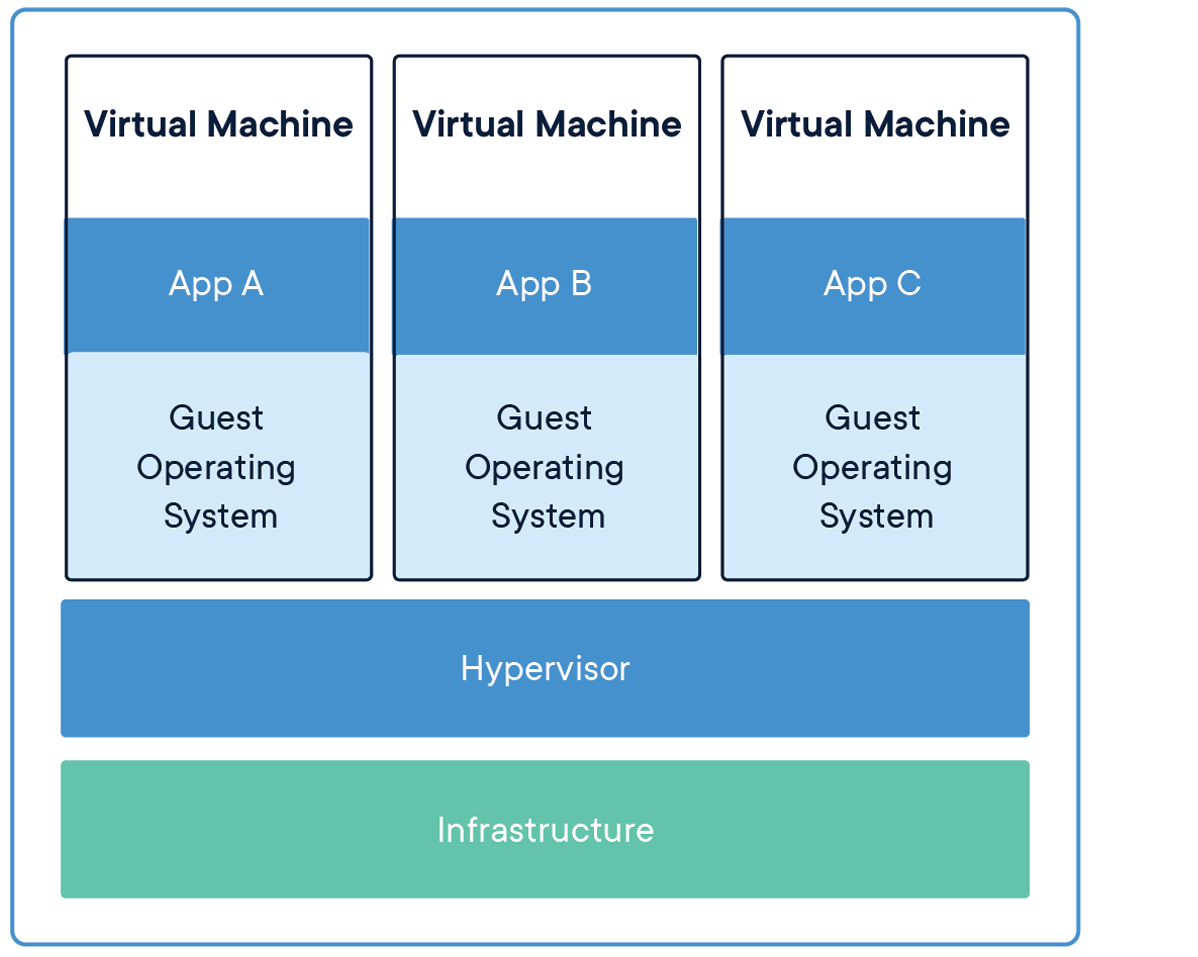
\includegraphics[width=0.5\linewidth]{vm_arch.png}
                    \caption[VM Setup]{Image portraying the general architecture of a VM-oriented setup. \cite{bib:vm-setup-img}.}
                    \label{fig:vm-arch}
                \end{figure}

            \subsubsection{Containers} \label{sec:container-intro}
                Before beginning to discuss whether containers are suitable for our purpose, we should begin by describing what a \textit{container} really is as it can be a confusing actor in the virtualization realm. Please note this section has been purposefully written as a high-level description of container technology. As stated before, a more technical discussion is presented on section \ref{sec:container-techy} belonging to chapter \ref{chap:2}.\\

                According to docker's documentation \cite{bib:docker-doc}, ``a \textit{container} is a standard unit of software that packages up code and all its dependencies so the application runs quickly and reliably from one computing environment to another''. Now, this definition is a perfect representative of the main kind of problems we will have to face when trying to bend containers to our will throughout the development process. Containers are designed to try and increase the portability of applications. In today's Internet-centric society, where we all want uninterrupted services, it is critical to be able to change an application's environment at a moment's notice due to outages, ending support cycles for software, security breaches... That is why the container technology has developed at such a high pace. It provides the infrastructure for a reliable service delivery. Now, we could ``twist'' the definition if we were to think of applications as full-fledged operating systems. That is, if we run a whole OS within these containers we would be actually achieving our goal: each container will behave as a network node so, in other words, we would only need to cope with $36$ concurrent containers: an easier task than doing the proper thing with VMs.\\

                One of the questions we asked ourselves when trying to decide on a technology was: what makes a container different than a VM? If we go back to the section we devoted to virtual machines we will notice how they run a full-fledged operating system as a guest. This implies each VM has its own \textit{kernel}. This is clearly shown on figure \ref{fig:vm-arch}.\\

                Kernels and their design have been the topic of many books and documents. We just need to know that the \textit{kernel} is the piece of software ``gluing'' the hardware and user-land software (programs such as browsers) together. That is, it allows applications to access the computing resources in an organized manner, enabling the sharing of resources amongst them. As we are telematics engineers we usually find the \textit{kernel} concept easier to understand in terms of the abstractions it offers us; the network socket being the most familiar. Through it, our applications can leverage the networking capabilities of the machine they're running on for instance.\\

                Unlike VMs, containers all share a single \textit{kernel}. We can then think of containers as a way of isolating applications along with all their dependencies within a shared computing platform. We don't need ``specialized'' software agents such as an hypervisor; we would only need to be very meticulous and know the \textit{kernel's} offered facilities very well to achieve the end result offered by containers. Projects like \textit{bocker} \cite{bib:bocker} prove one can achieve similar results to the ones provided by docker if only interested in a subset of the latter's capabilities. Nonetheless, one can regard containers as light VMs throughout the development as, even though it is not exactly true, it won't hinder our development approach. Figure \ref{fig:container-arch} shows the overall architecture of a container-based approach. Comparing it to figure \ref{fig:vm-arch} can be truly revealing when comparing both virtualization approaches.\\

                \begin{figure}
                    \centering
                    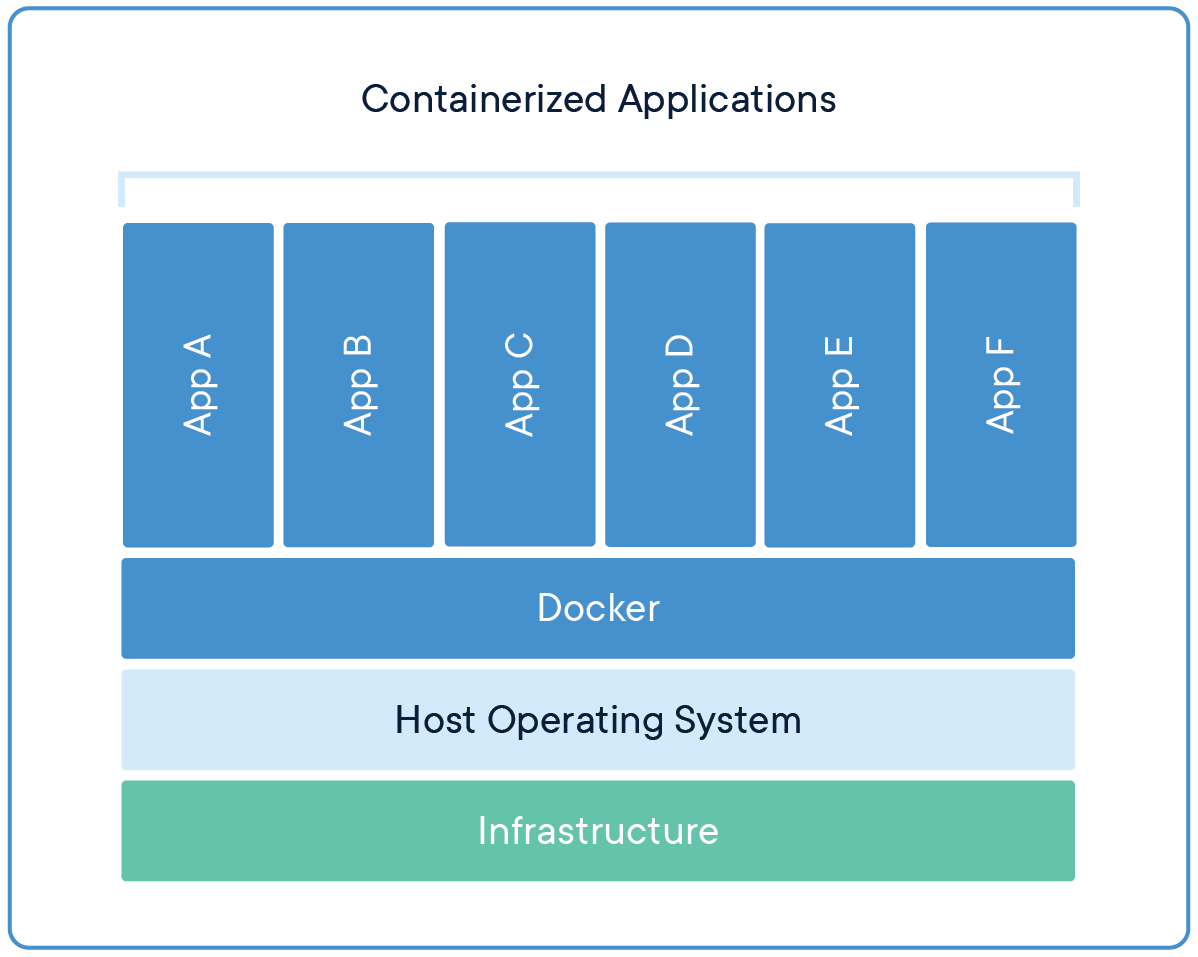
\includegraphics[width=0.5\linewidth]{container_arch.png}
                    \caption[Container Setup]{Image portraying the general architecture of a container-oriented setup. \cite{bib:container-setup-img}}
                    \label{fig:container-arch}
                \end{figure}

                \paragraph{Containers and Docker}
                    Container technology can be thought of as a standard. However, the way that technology is implemented can vary. Then, docker offers an \textit{implementation} for containers. This is a similar situation to that of VMs. The idea of a virtual machine has found two main implementations by VirtualBox and VMWare. This concept is similar to the situation posed by RFCs published by the IETF. They propose a standard and several people try to implement it according to their coding style, level of knowledge...

                    If we are to be entirely correct when it comes to nomenclature we would have to say that our solution is going to be based on docker's \textit{container implementation}.\\

                On top of container technology being lighter than that of VMs, which makes it more scalable, we also found the amount of documentation regarding the network infrastructure to be much larger. That gave us a strong foothold in our path to getting our framework up and running. Another positive aspect on containers we initially considered was the existence of \textit{container orchestration tools} such as \textit{Kubernetes} which we thought could make our job easier. We'll devote a few paragraphs to discussing why, in the end, \textit{Kubernetes} wasn't that much of a fit for us.

            \subsubsection{Kubernetes}
                As stated in \textit{Kubernetes'} own documentation \cite{bib:kubernetes-doc}, ``\textit{Kubernetes} is an open source container orchestration engine for automating deployment, scaling, and management of containerized applications''. In other words, \textit{Kubernetes} let's us define how we want our application to behave through a manifest provided in a \texttt{*.yaml} formatted file. Now, if we consider docker to be focused on offering ``services'', \textit{Kubernetes} takes that objective to the next level. It's a product aimed at professionals that's engineered to be stable. That means that meddling with the internals in an effort to achieve our goals was bound to be an extremely difficult task. By employing \textit{Kubernetes} we would be using an infrastructure that's already been laid for us, which is difficult to change and that does not behave how we want it to. We believe using a tool only to work against its basic principles is a wrong approach. That's why we decided to manually build the needed infrastructure from the ground up starting from docker containers.\\

                Just to give a concrete example of what we mean by working against the pre-existing infrastructure we could take a look at how \textit{Kubernetes} connects nodes. As it needs to offer some kind of service it will set up the internal network topology in such a way that all the nodes are able to connect among themselves. Given our requirement of implementing a firewall in the topologies we need to be working with, we can conclude it would be cumbersome to try to implement a firewall in an infrastructure whose primary concern is enabling communication links amongst all the network nodes. It's this diametrically opposite approach that made us dismiss \textit{Kubernetes} as a feasible solution.\\

        \subsection{Getting the Operating System}
            After settling on an option providing the ``hardware'' our software is to run on, we need to decide which operating system is the best suited for the task we have been proposed. Given today's ecosystem we quickly thought of the three main contenders in the user market. These are \textit{Microsoft Windows}, \textit{macOS} and \textit{Linux}. Before delving any deeper into the discussion about which to employ we would like to clarify our choice of words when referring to the last option.\\

            \paragraph{Linux vs. GNU/Linux}
                Strictly speaking, Linux is just the kernel of Linux-based distributions or \textit{distros}. As we explained in the previous section, a kernel is the piece of software gluing the hardware and user software together. It accomplishes this non-trivial feat by offering applications an interface through which they can request services. This kernel will then fulfill these requests in an orderly manner so that applications can coexist and cooperate towards a better overall usage of the system. These applications can in fact not even be aware that they are running alongside others.

                The kernel is for many the most crucial piece of software within a full fledged operating system. It's the cornerstone on which everything else is built. Nonetheless, if a non-technical user were given just a kernel they would have a very hard time making any use of it. This is where applications or user programs come into play. The make use of the OS's services and they let an end-user get meaningful work done. These end user programs range form text editors such as \texttt{vim} or \texttt{Microsoft Word} to VoIP (Voice over IP) PBXs (Private Branch eXchanges) like \texttt{asterisk}.

                The role of GNU in all this is providing many of these end user programs as free (as in freedom) software. Huge projects like the \texttt{gnome} desktop environment and \texttt{make} (which we are using for compiling this \LaTeX file) carry the GNU stamp. Given the above, GNU argues operating systems packaging their tools should be considered GNU/Linux systems as these two terms work cooperatively, i.e. they are software pieces with distinct purposes. While we consider this to be absolutely true for end-user systems such as \texttt{Ubuntu desktop} and \texttt{Debian} we feel this is not the real case with us.

                We will be running our network nodes as docker containers and we will try to make the image ran by these containers as lightweight as possible. In doing that we will only rely on GNU's shell, \texttt{bash}, for running a very restricted collection of commands. That is why we will refer to our platform as Linux containers instead of GNU/Linux ones.

            Knowing we have already restricted ourselves to the use of container technology we can discard \textit{macOS} as an option right away as there is no official support for it. We could have used \textit{Windows}-based containers but given our uncommon requirements we opted to use a \textit{linux}-based one. Given we feel comfortable with it, we settled on using \textit{Ubuntu} docker images for running our nodes. The version we employed during the testing phase was deemed \texttt{Bionic Beaver} and had version number \texttt{18.04 LTS} (Long Term Release) which boasts a higher stability than yearly versions. Given our requirements, all our work should run ``just fine'' on newer versions. We nonetheless recommend working to \texttt{LTS} releases as the yearly builds can sometimes behave unexpectedly. On top of our choice's flexibility, we mustn't forget about the price and licensing factors. Even though we haven't looked into these topics regarding Microsoft's OS, Windows licenses tend to be more restrictive than those attached to Ubuntu. As we plan on working at a very ``low level'' with the kernel's internal network infrastructure we aren't entirely sure if that would be allowed by Window's license terms. On top of that Ubuntu doesn't cost anything, so we won't have to be concerned about a monetary budget. Putting it all together justifies why we decided to run Ubuntu within our own containers.

        \chapter{Used Technology Analysis}
    According to the discussion in the previous chapter we have settled on docker containers running Ubuntu for providing the backbone of our virtualized networks. Now, once we are clear so as to what technology to employ we need to get down to the nitty gritty of implementing a full-fledged virtual network infrastructure. In order to do so we need to become acquainted with the Linux kernel.

    \section{Enter the Network Stack}
        A fascinating but rather messy image is \href{https://upload.wikimedia.org/wikipedia/commons/5/5b/Linux_kernel_map.png}{Linux's "Map"}. If we pay close attention we'll see how one of the columns is just devoted to networking. The software entities comprising this column is what we will refer to as \textit{Linux's Network Stack}\\

         The word stack is something that shows up time and time again in the area of networking. It helps us have a top-level view of how logical entities cooperate within a network. When we think about stacks we naturally begin to consider them in terms of the layers composing them with each layer tackling a simple task and offering services to the layer above whilst using those provided by the layer below. It's not going to be any different with Linux; we can think of its network stack as a huge "blob" of code which all network packets reaching a Linux-based system traverse. Thus, if we can alter how Linux processes packets or build "virtual" connections between different network stacks we would be capable of constructing a de-facto virtual network tailored to our needs.\\

         \paragraph{Naming Packets}
            Before we go on we need to shed some light on the naming we are going to use regarding the units of data exchanged through network links. Even though the term packet tremendously generic we feel it's not a wrong one to turn to in our case. When we wire up several network nodes together we are looking for full connectivity, that is, connectivity at the application level. Thus, we are not really that interested on what layer the "packet" is at, we don't really care if the packet is a \texttt{segment}, \texttt{datagram} or \texttt{frame}. In the case a need for more specific naming turns up we won't hesitate to use it but we prefer to keep the writing simple and avoiding getting bogged down with technicalities where we feel the benefit is not that obvious.

            A prime example of the above would be the use of the term \texttt{packet} instead of \texttt{link-layer frame} in the section's introduction. \texttt{Frame} is the correct term for referring to the data structure a \texttt{NIC} (Network Interface Card) hands to the kernel (albeit somewhat processed as the preamble and Frame Check Sequence of Ethernet frames are usually stripped from incoming frames by the \texttt{NIC} itself as seen \href{https://gitlab.com/wireshark/wireshark/-/wikis/Ethernet}{here}).

        If we think about network stacks, we would probably believe we need to have one per machine. That is, every network-capable devices must have their own \textit{data-path} which packets are to traverse. What may not be so simple is thinking that a machine \textit{may} have more than one network stack. In order to get a firmer grasp on the implications of the above idea let's revisit the world of network interfaces.\\
        
        When we first started learning about network architectures we where boggled by the fact that a machine could have more than one NIC. This implied it had several different IP addresses "attached" to it which provided redundancy amongst other several capabilities like traffic control. What astonished us the most was the raw power of not imposing a limit on the number of NICs a machine could have. That simple fact allowed routers to exist for instance and you could do "silly" stuff such as getting a packet through an interface and \texttt{echoing} it out the other. All in all, it provided loads of flexibility to the whole system.\\

        Now, if we transpose the above to the concept of network stacks we could be talking about packets being interchanged in between them whilst residing on the same machine nonetheless. If we sit back and take a look at the larger picture we can clearly see that packet exchanges below the application level are logically exchanged between network stacks belonging to different machines as it's the stack who's in charge of processing said data structures. Seeing matters in that light and knowing we can have several network stacks on a single platform, talking about packets being interchanged within a machine doesn't seem that far fetched now.\\

        Given the previous discussion we can now clearly see the base on which everything else is built upon. The ability to have several coexisting network stacks on a machine and being able to connect them as we please is such a powerful tool that our work is only scratching the surface of the capabilities enabled by this kind of technology. Linux's network stacks are nothing short of an ode to code modularity if you ask us.\\

        All the previous discussion is related with the theoretical or conceptual realm of matters. We will now delve into how we can translate these ideas into a working virtual network. After going through that process we'll also look into how we decided to do everything manually once we have a broader technical background on the subject.\\

        Finally, we feel we need to clarify that, even though it may be clear at this point, all the network traffic we are to generate originates from within our own system. In other words, our network would be perfectly capable of working without any Internet access.\\

    \section{The Network Namespace}
        % \pyfile{Code_snippets/foo.py}

        % Just as we have previously discussed, design and implementation are two very different things. A prime example is the case of the \texttt{SNMP} tools where \texttt{SNMP} stands for \texttt{Simple Network Management Protocol}. This protocol was originally defined in \href{https://tools.ietf.org/html/rfc1067}{RFC 1067} but no implementation was defined. With time, the \texttt{net-snmp} suite of tools became the de-facto implementation for \texttt{SNMP}. It is then of the utmost importance to notice that the design and implementation needn't be carried out by the same people; in fact, it's not uncommon to have several implementations for a given design. That's the case with shells of which we have so many, \texttt{bash}, \texttt{zsh}, \texttt{ksh} and so on. Then, we can expect the Linux...\\

        Many of the programming languages dominating today's market are object oriented. This, very roughly, means that the programmer is expected to generate \textit{classes} representing "real-life" entities to some extent. These classes are defined by their \textit{attributes} (characteristics) and their \textit{methods} (what they can do). Now, a class by itself cannot do anything, we need to \textit{instantiate} it so that we create an \textit{object} of that class. We'll then be capable of using the newly created object as we please.\\

        This concept on instantiation is actually quite powerful as it appears continuously in many areas of engineering. Now, we could say that Linux's network namespaces work in a similar fashion to classes. We can think of the network stack as the class and what we call \textit{network namespaces} as the objects. Let's delve a bit deeper into what these namespaces really are.\\

        As seen \href{https://en.wikipedia.org/wiki/Linux_namespaces}{here}, namespaces are not only seen when doing networking stuff, they are a feature of the Linux kernel employed in many other areas. These namespaces let us partition kernel resources so that each process sees a resource that's only for it, it's not shared. When applied to networking we can see how each network namespace represents an entire network stack. Then, if we set up several network namespaces (namespaces from now on as this is the only type of namespace we will deal with) we have effectively housed several network stacks under the same roof. If there was any way of interconnecting these namespaces we would have taken quite a dent off our task.\\

        We will now take a look at the virtual wires we have fought so many times against, the so called \texttt{veths}.\\

    \section{Wire time}
        In a previous section we already provided some comments on what NICs are. Knowing that interfaces create "bridges" between different systems we can clearly see how these network interfaces bridge digital systems to a communication network; they let these digital machines leverage the communication capacities of computer networks.\\

        Whilst almost all engineers could recognize what a NIC physically is, the matter is not that simple regarding how the OS treats these interfaces. We find it quite helpful to think of what we would do if we had to implement some software solutions that had to employ network's capabilities. There must be a "way" that these hardware components can be used from the application perspective, that is, the OS needs to offer some kind of abstraction through which we can make use of the NIC itself. This abstraction is what we will call a OS-level NIC or network interface.\\

        Before delving any deeper into this matter we need to discuss what the \texttt{iproute2} suite is as we believe adding some examples to the contents to follow would really enrich them.

        \subsection{Meeting \texttt{iproute2}}
            The time we spend on terminal emulators has exponentially increased as we worked our way through our bachelor's. Even though they provide quite a fast way to "get around" the computer they can be a little abstract at times. We are always aware that the OS "under" us has many running processes and provides us with services that can be used at our request. The thing is, faith can at times be scarce so we usually have tools that can inform us about what's going on "behind the scenes". This is the case for programs like \texttt{ps} which reports the status of the system's processes or \texttt{w} which tells us about who is currently logged on the system as well as what they are up to. When using a shell we are aware of the fact that other processes are running and that other users may be logged on but we nonetheless have tools that let us consult the current status of the system.\\

            Where networking is concerned, \texttt{iproute2} is like a Swiss Army Knife. It's a \textit{suite} or collection of tools that lets us do everything from inspecting the current interfaces and routes to generating \texttt{IPv6/IPv4} tunnels. We'll only be concerned with the \texttt{ip} command in our case which is in charge of "showing / manipulating routing, network devices, interfaces and tunnels" as seen in \texttt{ip}'s manpage (which can be consulted with \texttt{man ip}).
        \chapter{Manually Bringing Up a Simple Network} \label{chap:3}
    \epigraph{If the vendors started doing everything right, we would be out of a job.
    Let's hear it for OSI and X!  With those babies in the wings, we can count
    on being employed until we drop, or get smart and switch to gardening,
    paper folding, or something.}{\textit{C. Philip Wood}}

    Figure \ref{fig:sample-topology} showcases a simple topology we will instantiate by applying the contents described in chapter \ref{chap:2}. Instead of relying on our framework to perform the task, we will manually carry out all the needed steps and detail them in a code listing. This demonstrates how are tool is nothing more than an additional ``layer'' in charge of managing the subtleties we will manually deal with once the topologies' complexity begins to increase.\\

    \section{A Note on the Chosen Private IP Range}
        As seen on section $3$ of \cite{bib:rfc1918} we could have chosen private addresses within one of $3$ private network address spaces. Doing so guarantees we will not run into any collisions should we want to let our virtual hosts and routers communicate with the public Internet. We should nonetheless be aware of the fact that, if we are pursuing a completely isolated virtual network we need not adhere to these reserved address ranges: no collisions could probably occur.\\

        Given we did not have a firm reason not to choose one of the reserved private address spaces, we decided to make use of them. As our home network uses the \textit{192.168.1.0/24} range and, in our experience, the \textit{172.16.0.0./12} space tends to be more common, we decided to assign addresses within the \textit{10.0.0.0/8} pool. These are the ones that will be included in any figures and listings that need to explicitly include IP addresses.\\

    \begin{figure}
        \centering
        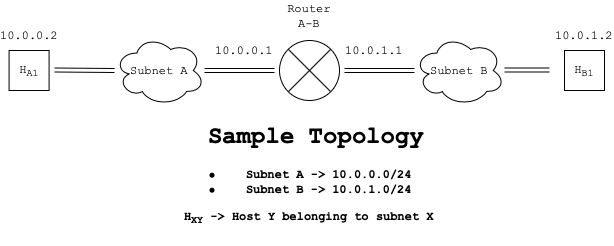
\includegraphics[width=\linewidth]{sample_topology.png}
        \caption[A Sample Topology]{The Sample Topology We Will Set Up Throughout Chapter \ref{chap:3}.}
        \label{fig:sample-topology}
    \end{figure}

    \section{Automating the Sample Topology}
        Listing \ref{lst:sample-topology} contains the shell script automating the deployment of the network showcased on figure \ref{fig:sample-topology}. The script itself contains messages that are to be printed to the user which clarify its operation to a great extent.\\

        \subsection{Running the Script}
            As seen on \textit{line 1} of listing \ref{lst:sample-topology} this script is to be tun within a \textit{bash} shell. This can be accomplished in one of two ways as shown on \ref{lst:bash-script}. As we will later look into, the script is to be run by \textit{root} so that it can carry out the needed operations. This amounts to prepending the command we choose to run the script by \texttt{sudo}.\\

            \begin{lstlisting}[language = bash, caption = Running a \textit{bash} Script., label = lst:bash-script]
                # Making the script executable and running it.
                chmod +x <script-name> && sudo ./<script-name>

                # Spawning a privileged shell and running the script in it.
                sudo bash <script-name>
            \end{lstlisting}

        \subsection{Checking the Script is Run by root}
            The privileged user in \textit{UNIX}-based systems is identified by a \textit{UID} (User ID) of $0$. When a program is run, the associated process will have the \textit{UID} of the user who launched it. Some program's permissions allow it to run with a different \textit{UID} than that of the user executing it: this is wha we call the \textit{EUID} (Effective \textit{UID})). In any case, if the \textit{EUID} of a process evaluates to $0$ it is being run by \textit{root}. This is what is being checked by \textit{lines 3-7} on listing \ref{lst:sample-topology}. If the user running the script is not \textit{root} we will simply abort execution whilst warning the user.\\

        \subsection{Automatically Tearing Down the Topology}
            As seen in \textit{lines 9-17}, the script shown on listing \ref{lst:sample-topology} is prepared to dismantle the network topology it brings up when invoked a second time. The trigger for this behaviour is passing a parameter when running the script. Any parameter will cause the removal of the entire virtual network: this is not the best practice when writing code but it simplifies handling the arguments passed to the script. We are concerned with clearly portraying the technologies discussed in chapter \ref{chap:2}, not with teaching the user how to write proper shell scripts. In any case, running \texttt{sudo bash <script-name> quit} will dismantle the sample virtual topology.\\

        \lstinputlisting[language = bash, caption = Automatic Deployment of the Sample Topology., label = lst:sample-topology]{Code_snippets/sample_topology.sh}

    \section{Testing the Topology Is Working}
        Once the script shown on listing \ref{lst:sample-topology} has been run we should have a full-fledged virtual network at our disposal. The simplest way to check we do have full connectivity is checking one of the hosts can ``see the other''. we can accomplish our objective by running a shell within one of the hosts and then trying to \textit{ping} the other. We can extract the appropriate \textit{IP} addresses from figure \ref{fig:sample-topology}. Listing \ref{lst:sample-topology-test} shows how we can open up a shell within host $H_{A_1}$ and launch \textit{ping} against host $H_{B_1}$.\\

        \begin{lstlisting}[language = bash, caption = Testing the Sample Topology., label = lst:sample-topology-test]
            # Spawn a shell within H-A-1
            docker exec -it h-a-1 bash

            # Ping H-B-1 3 times from H-A-1
            root@h-a-1:/$ ping -c 3 10.0.1.2

            # It should produce an output similar to:
                # PING 10.0.1.2 (10.0.1.2) 56(84) bytes of data.
                # 64 bytes from 10.0.1.2: icmp_seq=1 ttl=63 time=0.036 ms
                # 64 bytes from 10.0.1.2: icmp_seq=2 ttl=63 time=0.057 ms
                # 64 bytes from 10.0.1.2: icmp_seq=3 ttl=63 time=0.062 ms
                #
                # --- 10.0.1.2 ping statistics ---
                # 3 packets transmitted, 3 received, 0% packet loss,\
                    # time 2049ms
                # rtt min/avg/max/mdev = 0.036/0.051/0.062/0.011 ms

            # We can also run traceroute
            root@h-a-1:/$ traceroute 10.0.1.2

            # It should produce an output similar to:
                # traceroute to 10.0.1.2 (10.0.1.2), 30 hops max, 60\
                    # byte packets
                # 1  10.0.0.1 (10.0.0.1)  0.029 ms  0.039 ms  0.007 ms
                # 2  10.0.1.2 (10.0.1.2)  0.018 ms  0.023 ms  0.041 ms
        \end{lstlisting}

    Now that we have shown how to ``manually'' set up a simple network we begin to discover the challenges that will surely arise as their complexity grows. What is more, we also need to add additional functionalities such as moving end nodes around the network in a way that does not mangle the network's operation. The next chapter is devoted to providing a high level overview of our tool's design and operation together with a comprehensive collection of the actions it can and cannot perform.

        \chapter{Automating the Deployment of Virtual Networks} \label{chap:4}
    \section{High Level Overview}
        As seen in chapter \ref{chap:3}, bringing a virtual network up entails an organizational overhead that is not easily handled. That is why we have developed a complete software system capable of handling these intricacies in an automatic fashion. Then, a user need only provide a \texttt{graph} describing the desired topology and our project will be able to read, interpret and instantiate said network.\\

        Due to its simple yet rich syntax, we have decided to leverage the \textit{Python} \cite{bib:python} programming language to develop the entire system. We will be using version \texttt{3.x} given \texttt{python}'s \texttt{2.7} release has been deprecated as of \textit{January 2021}. One of the external dependencies we will make use of is the \textit{NetworkX} \cite{bib:networkx} network analysis module. This software bundle was recommended by the research group we have collaborated with and it is distributed as a \texttt{python package}. Thus, we felt even more inclined towards \texttt{python}. Given we will interact with the \texttt{docker engine} through its \texttt{CLI API}, its use will not impose any restrictions on our choice either. This implies that we have nothing more than reasons supporting the use of \texttt{python} for our development.\\

        \subsection{External Dependencies}
            One of the main objectives pursued throughout the development was reducing the number of external dependencies to the maximum extent. We did manage to only require the presence of \texttt{docker}, \texttt{iproute2} and \texttt{python3} for an initial and fully functional version. Not leveraging \texttt{NetworkX} implied we had to manually route all the nodes within the network, which amounted to be a rather complex task. Due to the research group's suggestions we settled on taking advantage of \texttt{NetworkX} for both modeling the different topologies and routing them. Then, we have designed two independent solutions that accomplish the same task. One of them \textbf{does not} require \texttt{NetworkX} whist the other one \textbf{does}. The reasoning behind including a dependency that is not strictly needed is that it greatly simplifies our code and it will surely avoid some of the most common pitfalls our own solution can incur into under complex circumstances.\\

            The following enumeration briefly explains the use of each of the required dependencies. Please bear in mind that the installation instructions for each of them are detailed in the document's appendix.\\

            \begin{enumerate}
                \item \textbf{\texttt{Python3}:} With \texttt{python3} being an interpreted language, we need to make use of the interpreter that is going to execute our code.
                \item \textbf{\texttt{Docker}:} The different nodes in our network are modeled as \texttt{docker containers}, which implies we indeed depend on \texttt{docker} for making our system work.
                \item \textbf{\texttt{IpRoute2}:} We need the \texttt{iproute2} suite of tools to manage the virtual networking infrastructure ``gluing'' all our nodes together.
                \item \textbf{\texttt{NetworkX}:} As explained above, we \textit{are not forced} to use \texttt{NetworkX} and we have developed a version that does not depend on it at all. Nonetheless, it does simplify big portions of code and so we decided to include it in our final, sharper version.
                \item \textbf{\texttt{Matplotlib}:} \texttt{NetworkX} is capable of graphically representing our topologies through \textit{graphs}. In order to ``draw them'', \texttt{NetworkX} depends on the \texttt{matplotlib} module we have also installed as a dependency. This module is however \textbf{not mandatory}: they rest of the program will work as intended, it will just be unable to graphically represent the topology. In a later chapter we will devote our time to looking into a \textit{proof of concept} we have developed. Said experiment generates a series of time-tagged events that our program is capable of representing as a regular graph. The lack of the \texttt{matplotlib} module implies this graph will not be available either. All in all, it is up to the user to decide whether they want this functionality or not: the program itself will carry out is primary task either way.
                \item \textbf{\texttt{Docker Python SDK}:} We \textbf{have not} used the \texttt{docker python SDK} (\texttt{S}oftware \texttt{D}evelopment \texttt{K}it) in our project. We have decide to leverage \texttt{docker}'s \texttt{CLI} interface from our code through calls to \texttt{os.system()}. However, someone deciding to use our project as a basis for something else might feel more comfortable interacting with \texttt{docker} through a pure-\texttt{python} \texttt{API} (\texttt{A}pplication \texttt{P}rogramming \texttt{I}nterface). Changing our code to work in said fashion is a rather simple task should it have to be done.
            \end{enumerate}

        \subsection{User Manual}
            Throughout the development of our tool we have tried to simplify the use of the project as much as possible. The end result is a user-side workflow that only requires them to import a single project module to which they \textbf{must} provide a \texttt{NetworkX graph}. After doing so, they will be presented with a simple \texttt{CLI} letting them modify the currently live virtual network.\\

            \paragraph{User Permissions}
                Given the project will make use of \texttt{iproute2} the program needs to be run with administrative privileges (i.e. prepended by \texttt{sudo}). Even though this is the easiest approach and everything will ``just work'' it does have some security implications (mainly command injection) we will showcase in the appendix. Instead of choosing to run the entire blob of code as \texttt{root} we can also grant certain capabilities to the user who is to run the code, namely the \texttt{NET\_ADMIN} capability (the same we need to grant containers). We should also mention that the user running the program must be able to interact with the \texttt{docker engine}. This can be ensured by adding said user to the \texttt{docker group} within the system, even though \texttt{root} will also be able to interact with and manage containers. This paragraph is intended as a warning, please refer to the appendix for a deeper discussion.\\

            Depending on how the users decide to provide the required \texttt{graph} they might need to import additional modules. If they have stored a live graph as a \textit{pickle} \cite{bib:python-pickle} they will then need to import the \textit{pickle} module to \texttt{un-pickle} the graph, for instance. In our examples we will define the graphs ``on-the-fly'', which requires us to import \texttt{networkx} itself. Listing \ref{lst:sample-topology-graph} shows how one would define the topology found on figure \ref{fig:sample-topology} as a \texttt{networkx} graph.\\

            \begin{lstlisting}[language = python, caption = Defining the Sample Topology as a \texttt{networkx} graph., label = lst:sample-topology-graph]
                # Import the networkx module so that we can define a graph.
                import networkx

                # Instantiate the netowrkx.Graph class.
                sample_net = networkx.Graph(net = 'Sample Topology')

                # Add host H-A-1 and the bridge for subnet A.
                sample_net.add_node('h-a-1', type = 'node')
                sample_net.add_node('subnet-a-brd', type = 'bridge', subnet = '10.0.0.0/24')

                # Add host H-B-1 and the bridge for subnet B.
                sample_net.add_node('h-b-1', type = 'node')
                sample_net.add_node('subnet-b-brd', type = 'bridge', subnet = '10.0.1.0/24')

                # Add the R-A-B router with NO firewall rules.
                sample_net.add_node('r-a-b', type = 'router', fw_rules = {})

                # Connect H-A-1 to the bridge for subnet A.
                sample_net.add_edge('h-a-1', 'subnet-a-brd')

                # Connect H-B-1 to the bridge for subnet B.
                sample_net.add_edge('h-b-1', 'subnet-b-brd')

                # Connect router R-A-B to both bridges.
                sample_net.add_edge('subnet-a-brd', 'r-a-b')
                sample_net.add_edge('subnet-b-brd', 'r-a-b')
            \end{lstlisting}

            \subsubsection{Creating Well-formed Graphs} \label{sec:good-graphs}
                Our tool expects the nodes on a \texttt{networkx} graph to adhere to certain constraints so that it can assemble the requested topology. Given the bi-directional nature of network links (data is sent in both directions), we have decided to model our networks as \textbf{undirected graphs}. Then, these will always be composed by a set of \texttt{nodes} interconnected by a set of \texttt{edges}. The types of nodes one can use are listed on table \ref{tab:node-types}.\\

                \begin{table}
                    \centering
                    \begin{tabular}{|c|c|}
                        \hline
                        \textbf{Node Type} & \textbf{Description}\\
                        \hline
                        \texttt{node} & A regular host.\\
                        \hline
                        \texttt{bridge} & A link-layer switch that represents an entire subnetwork.\\
                        \hline
                        \texttt{router} & A net-layer router joining two or more subnetworks together.\\
                        \hline
                    \end{tabular}
                    \caption{Node types.}
                    \label{tab:node-types}
                \end{table}

                When adding a new node one must make sure that the following constraints \textbf{are respected}. Otherwise, all sorts of undefined behavior can and will be experienced: anything from a network that cannot be started to the presence of routing loops can happen. Given the restrictions we are imposing, these will be \textit{bipartite graphs} \footnote{\label{ft:bigraphs}https://en.wikipedia.org/wiki/Bipartite\_graph}. Using the same notation as footnote \footnotemark[\value{footnote}], set $V$ would contain bridges whilst set $U$ would contain both nodes and routers. This property \textbf{has not} been leveraged in our code, but it could prove to be useful if this work is developed further.\\

                \begin{enumerate}
                    \item \textbf{Rules regarding node definitions:}
                    \begin{enumerate}
                        \item Each node's name \textbf{MUST} be a \textbf{unique} \texttt{string}.
                        \item Each node \textbf{MUST} contain a \texttt{type} attribute whose value is a \texttt{string}.
                        \item The value of the \texttt{type} attribute \textbf{MUST} be one of \texttt{"node"}, \texttt{"router"} or \texttt{"bridge"}.
                        \item Each bridge \textbf{MUST} contain a \texttt{subnet} attribute.
                        \item Every value for a \texttt{subnet} attribute \textbf{MUST} be specified as a \texttt{string} with the \texttt{"A.B.C.D/E"} format, where $A,\ B,\ C,\ D \in [0,\ 255];\ E \in [0,\ 30]$.
                        \item The subnetwork ranges associated to each bridge through the \texttt{subnet} attribute \textbf{MUST} be \textbf{unique}.
                        \item Each router \textbf{MUST} contain a \texttt{fw\_rules} attribute.
                        \item Each \texttt{fw\_rules} attribute \textbf{MUST} be set to a \texttt{dictionary} complying to the specifications laid out in section \ref{sec:fw-rules}.
                    \end{enumerate}
                    \item \textbf{Rules regarding edge definitions:}
                    \begin{enumerate}
                        \item The \texttt{strings} used to identify the nodes to be joined by an edge \textbf{MUST} refer to previously defined nodes.
                    \end{enumerate}
                    \item \textbf{Rules regarding the topology:}
                    \begin{enumerate}
                        \item Each subnetwork is \textbf{MUST} be composed by a \textbf{single} switch and an arbitrary number of nodes and/or routers.
                    \end{enumerate}
                \end{enumerate}

            \subsubsection{Running a Graph} \label{sec:graph-exec}
                Once we have defined a graph as we have done on listing \ref{lst:sample-topology-graph} we just need to run it to turn it into a virtual network. This can be accomplished though the \texttt{launch\_net()} function we have defined on the \texttt{net\_tools} module. We will of course analyze these in a later section.\\

                Listing \ref{lst:running-a-graph} shows how a use can run an existing \texttt{networkx} graph like the one defined on listing \ref{lst:sample-topology-graph}.\\

                \begin{lstlisting}[language = python, caption = Turning a graph into a virtual network., label = lst:running-a-graph]
                    # Importing our module to launch the virtual network
                    from net_tools import net_ctrl

                    # This line will trigger the virtual network's creation.
                        # The second parameter controls whether we enable
                        # the configured firewalls or not.
                    net_ctrl.launch_net(sample_net, fw_on = False)
                \end{lstlisting}

            \subsubsection{Configuring Firewalls} \label{sec:fw-rules}
                When configuring router \texttt{R-A-B} on listing \ref{lst:sample-topology-graph} we passed an empty \texttt{dictionary} \texttt{\{\}} to the \texttt{fw\_rules} parameter thus effectively disabling the firewall of said router.\\

                In order to define appropriate rules, the user needs to provide a \texttt{dictionary} adhering to the syntax specification shown on listing \ref{lst:fw-dict-syntax}. Note that the order in which these rules are specified is the order in which they will be instantiated. This \textbf{will not} affect our topologies, but it can have an impact on the logical connections supported on the virtual network infrastructures.\\

                \begin{lstlisting}[language = python, caption = Syntax for specifying firewall rules., label = lst:fw-dict-syntax]
                    # Note '|' is to be read as 'OR'
                    fw_rules = {
                        'POLICY': 'DROP' | 'ACCEPT',
                        'ACCEPT': [(RULE_1), (RULE_2), ..., (RULE_N)],
                        'DROP':   [(RULE_A), (RULE_B), ..., (RULE_Z)]
                    }

                    # Each rule has a syntax of the form
                    ('origin_node', 'destination_node', True | False)
                \end{lstlisting}

                \paragraph{Rule Syntax}
                    The first $2$ elements are \texttt{strings} containing the names of the origin and destination nodes, respectively. The third parameter acts as a flag controlling whether the rule is uni or bi-directional. If set to \texttt{False}, we will only instantiate a rule affecting traffic going from the origin to the destination. If it is \texttt{True} however we will also instantiate a symmetric rule allowing for two-way communication. Even though the flag is not \textit{explicitly} needed it does reduce the configuration specification tremendously, as the topologies we worked with always made use of symmetric rules. Listing \ref{lst:sym-vs-uni-fw} shows how one can accomplish the same configuration with two rules instead of one if not using said flag.\\

                    \begin{lstlisting}[language = python, caption = Uni-directional vs. symmetric firewall rules., label = lst:sym-vs-uni-fw]
                        # Enable two-way communication x <--> y.
                        ('x', 'y', True)

                        # This accomplishes the same result with two triplets.
                        ('x', 'y', False)
                        ('y', 'x', False)
                    \end{lstlisting}

                \paragraph{Dictionary Syntax}
                    The \texttt{dictionary} contains $3$ key-value pairs. The first one defines the policy for the \texttt{FORWARDING} chain as a \texttt{string}. The second one contains a \texttt{list} of rules for \texttt{ACCEPT}ing packets. If the default policy is set to \texttt{ACCEPT} these rules will be meaningless... The third one contains a \texttt{list} of rules for \texttt{DROP}ping packets. If the default policy is to \texttt{DROP} them these rules will have no effect either.\\

            \subsubsection{Execution Modes}
                Chapter \ref{chap:5} is devoted to analyzing the \textit{proof of concept} we have developed. Said \textit{proof of concept} will produce a series of files \texttt{CSV} containing data that characterizes how the experiment developed. These files can also be analyzed by our program to provide a nicely formatted output so that the end user can make the most of the results.\\

                Instantiating a full-fledged virtual network when the user only wants to load some \texttt{CSV} files to graph or analyze them can prove to be a rather time and energy consuming process. That is why we have developed the so called \textit{report mode} on top of the \textit{normal} or \textit{network mode}.\\

                The former will cause the program to parse a graph defining a network topology and then instantiate it. This mode can of course carry out the same analysis on files as the \textit{report mode}. The \textit{report mode} on the other hand will just present the user with the \texttt{CLI} where he or she will be able to invoke a subset of all the commands. These are: \texttt{ld-atk-data}, \texttt{atk-graph}, \texttt{c | clear}, \texttt{quit | exit | x} and \texttt{CTRL + C}.

                The advantage \textit{report mode} has over the \textit{normal mode} is that it need not be concerned with instantiating a virtual network. This makes its startup time almost negligible.\\

                In order to enable \textit{report mode}, one can either specify the \texttt{report\_mode = True} parameter on the call to \texttt{launch\_net()} as seen on listing \ref{lst:running-a-graph} or just run the \texttt{net\_ctrl.py} file directly with \texttt{python3 net\_ctrl.py}. The latter approach will trigger an \texttt{if name == "\_\_main\_\_:} clause, thus causing the \texttt{report\_mode} parameter to be set to \texttt{True}. Please note the different files and their purposes will be explained in a later section.\\

            \subsubsection{Available Commands} \label{sec:cli-cmds}
                As stated before, our tool will allow the users to modify the virtual network once it is up and running through a \texttt{CLI} interface. The following enumeration contains a list of the available commands together with a short description of what they can achieve.\\

                \begin{enumerate}
                    \item \textbf{\texttt{mvsubn <affected\_subnet> <destination\_subnet>}:} This command will move the \texttt{<affected\_subnet>} and attach it to the \texttt{\allowbreak<destination\_subnet>}. These identifiers should be the ones provided by the \texttt{lssubn}. If either subnet does not exist, the command will fail with an error message.
                    \item \textbf{\texttt{mvnode <affected\_node> <destination\_subnet>}:} This command will move the \texttt{<affected\_node>} to the \texttt{<destination\_subnet>}. These identifiers should be the ones provided by \texttt{lsnode} and \texttt{lssubn}, respectively. If either element does not exist, the command will print an error message.
                    \item \textbf{\texttt{lssubn}:} This command will print a list of all the currently active subnetworks. These identifiers are the ones to be provided to the \texttt{mvsubn} and \texttt{mvnode} commands.
                    \item \textbf{\texttt{lsnode}:} This command will print a list of all the currently active nodes. These identifiers are the ones to be provided to the \texttt{mvnode} command.
                    \item \textbf{\texttt{lsnet}:} This command will graphically represent the current network topology. Please note this call is blocking, so the user will not be able to issue any other command until he or she closes the image. This command will require the installation of the \texttt{matplotlib} dependency. It is also worth mentioning that the generated image can be stored as a \texttt{PNG} file for later inspection.
                    \item \textbf{\texttt{lscnx}:} This command will show a ``higher level graph'' capturing the logical connections set up through firewall rules within the routers belonging to the network. If firewalls have not been enabled, the command will just print an informative message on screen as the resulting graph would be the same as the one shown by the \texttt{lsnet} command, given no logical connections are hampered by firewall rules. Even though one can generate this graph, the user should regard it as more of a ``debugging'' feature. We are internally the data structure from which the graph is derived as means of making dynamic firewall reconfiguration easier.
                    \item \textbf{\texttt{dump-atk-data [path]}:} Running the attack on the scenario generates output through files within the network nodes. This command is in charge of reaping all this data an dumping it both to a file and to a \texttt{dictionary}. Please note that, as the main program is ran as \texttt{root}, the generated files will belong to said user. One can manually change permissions with \texttt{chown} later on. These files contain a list of comma separated values (that is, these are \texttt{CSV} files) that are human readable. Nonetheless, the primary intention of this files is to allow the user to later inspect them and generate graphs through the program itself. In order to do so, we have prepared the so called \texttt{report-mode}. As seen in the command description, one can optionally provide a path to save the file to under \texttt{\allowbreak ../proof\_of\_concept/generated\_data/}. This will usually be just a filename. If this path is not provided, the default name \texttt{last\_data.csv} will be used. Please note that results will overwrite themselves unless the user changes the output file's name.
                    \item \textbf{\texttt{ld-atk-data [path]}:} This command will load the attack data from the default \texttt{\allowbreak../proof\_of\_concept/generated\_data/last\_data.csv} file or the one specified through the optional \texttt{path} parameter. Please note that \texttt{\allowbreak ../proof\_of\_concept/generated\_data} will be prepended to whatever argument is provided. This command will fail if the provided path leads to a non existent file.
                    \item \textbf{\texttt{atk-report}:} This command will read the \texttt{dictionary} containing the attack's results and print a nicely formatted table to \texttt{stdout} showing the times the \texttt{ping} processes went either up or down. In order for it to work, the user must either dump the data previously through \texttt{dump-atk-data} or load it from a file with \texttt{ld-atk-data}. If these steps have not been fulfilled, a nice reminder will be printed to the screen.
                    \item \textbf{\texttt{atk-graph}:} This command will show a graph displaying the evolution of the number of \texttt{ping} processes in the network against time. As before, the data must either be dumped or loaded beforehand.
                    \item \textbf{\texttt{check-atk}:} This command was written to aid in the debugging of the attack script. It will display the number of times the attack has run on each network node. An attack that is behaving as expected will run only once within each node.
                    \item \textbf{\texttt{launch-pings}:} This command will launch a \textit{daemonized} \texttt{ping} process in each node. \textit{Daemonizing} the \texttt{pings} allows them to keep on running after the script moves to a new network node (i.e. it allows ping to run without a controlling \texttt{TTY}).
                    \item \textbf{\texttt{reset-net}:} The attack we have written relies on several output files it generates to keep track of its current state. Thus, running the attack twice may result in some unexpected behaviour. This command will get rid of said files so as to effectively restore the network nodes to their original state.
                    \item \textbf{\texttt{clear | c}:} This command will clear the screen to allow for a more comfortable user experience. If running on a compliant shell, the \texttt{CTRL + L} combination will have the same effect. Note this command can be invoked either via \texttt{clear} or just \texttt{c} as seen in the syntax specification.
                    \item \textbf{\texttt{quit | exit | x}:} This command will dismantle the network and exit the program. Note \texttt{exit} and \texttt{x} are \textit{aliases} for \texttt{quit}.
                    \item \textbf{\texttt{CTRL + C}:} This key combination will send the \texttt{SIGINT} signal to the process which will be handled, causing the program's termination. The user may need to press \texttt{ENTER} so that the program reads it, as the call to \texttt{input()} is blocking and sometimes interferes with the user's input.
                \end{enumerate}

    \section{In-depth Module Analysis}
        One of the principles driving software development is \textit{modularity}. We have then tried to make our code components as independent as possible whilst allowing them to cooperate so that they can be used for other purposes besides the ones that we originally intended.\\

        The development effort culminated on $3$ different modules fulfilling each a set of tasks:

        \begin{enumerate}
            \item \textbf{\texttt{virt\_net}:} This module is concerned with the instantiation of the different network elements (\texttt{veths}, \texttt{bridges} and \texttt{nodes}) together with their addressing and configuration. The module contains classes representing everything from the entire network to a single \texttt{veth}.
            \item \textbf{\texttt{graph\_interpreter}:} This module acts as an intermediary translating the graphs provided by users to instances of the different classes defined in the \texttt{virt\_net} module. It will also implement the high-level functionality provided by user commands such as \texttt{mvsubn} and \texttt{mvnode}. On top of that, it will leverage \texttt{networkx}'s functionality to route the entire network and instantiate said routes in the routers once they have been brought up.
            \item \textbf{\texttt{net\_ctrl}:} This module implements the \texttt{CLI} users running the tool will be presented with. It will resolve issued commands to calls to functions defined in the \texttt{graph\_interpreter} module. This module serves as the user's entry point to the functionality offered by our tool.
        \end{enumerate}

        The design we have just specified allows other users to ``swap'' the modules they do not desire to use for their own or third-party ones. One can, for instance, decide not to use our \texttt{graph\_interpreter} and manually instantiate a network through calls to the \texttt{virt\_net} module alone and that would be completely feasible. We will now include the documentation for each of the modules down to the \textit{function-level}.\\

        \subsection{Conventions}
            \subsubsection{Data Type Specifications}
                The \texttt{C programming language} is by no means user friendly. Nonetheless, there is one aspect we really missed when developing in \texttt{python}: data type specification. In an effort to make the understanding of our code easier we have decided to specified each attribute's and variable's data types in the documentation composing this section. The syntax we will use to describe the used types is:\\

                \begin{itemize}
                    \item \textbf{\texttt{Strings}:} \texttt{string}.
                    \item \textbf{\texttt{Lists}:} \texttt{list/value\_type}.
                    \item \textbf{\texttt{Dictionaries}:} \texttt{dictionary/key\_type/value\_type}.
                    \item \textbf{\texttt{Boolean}:} \texttt{boolean}.
                    \item \textbf{\texttt{Instance of class Foo}:} \texttt{Foo\_inst}.
                \end{itemize}

            \subsubsection{Defining Private Methods}
                One of the main advantages of the object-oriented programming is that it provides ``access control'' to methods and attributes of a class. In \texttt{C++}, this is accomplished by classifying them as \texttt{private} or \texttt{public}, for instance. On the other hand \texttt{python} does not \textit{enforce} this behaviour: a user will be able to call any method or access any attribute of an instance.\\

                In order to ``circumvent'' this issue, the convention has it that method and attribute names prepended by an underscore (\texttt{\_}) are to be treated as private. If a user decides to explicitly call or access these methods and attributes he or she is then exposed to undefined behaviours.\\

            \subsubsection{Calling Methods Through the Module Name}
                We have chosen to always call functions and instantiate classes external to the current file through their full name (i.e. including the name of the external file in the call). This does increase the length of code lines but it allows the reader (and ourselves) to know where the functions and classes are effectively defined. We feel like the increase in line length is completely justified.\\

            \subsubsection{The \texttt{\_\_init\_\_.py} File}
                Each of our modules contains an empty \texttt{\_\_init\_\_.py} file so that they become \texttt{regular packages}. This allows us to comfortably import the modules where their contents are needed. More information on \texttt{python}'s import system can be found on section $5.2.1$ of \cite{bib:python-import}.

            \subsubsection{Constructors and Destructors}
                When a \texttt{class} is instanced and it becomes an \texttt{object} one special method will be automatically invoked for us: the \texttt{constructor}. In \texttt{python} this method is \textbf{always} named \texttt{\_\_init\_\_()} and it \textbf{cannot} return anything.\\

                The counterpart of the \texttt{constructor} is the \texttt{destructor}. \texttt{Python} is \textit{garbage collected} in the sense that, once there are no more references to an object, it will schedule it for deletion. When an object is being deleted its \texttt{destructor} will be automatically called as well. This \texttt{destructor} is always defined as \texttt{\_\_del\_\_()} in \texttt{python} and it accepts a single argument: a reference to the instance that is being deleted (i.e. \texttt{self}). Just like the \texttt{constructor}, it \textbf{cannot} return anything.\\

                These methods will be defined for each of our classes and, given the \texttt{\_\_init\_\_()} and \texttt{\_\_del\_\_()} names can come across as rather cryptic we have decided to denote them as \texttt{constructor} and \texttt{destructor}, respectively, in the following sections.\\

        \subsection{The \texttt{virt\_net} Module}
            \subsubsection{Constants.py}
    In an effort to reduce the number of dependencies we decided to leverage \textit{ANSI Escape Codes} to colour the different output messages. This module then defines the different \texttt{strings} controlling the colours.

    \paragraph{Imported Libraries}
        None as there are no external dependencies.

    \paragraph{Global Variables}
        \begin{enumerate}
            \item \textbf{\texttt{terminal\_escape\_sequences (dictionary/string/string)}:} \texttt{Dictionary} keyed by color names whose associated values are \texttt{ANSI Escape Sequences} changing the terminal's output color to the one specified. This solution is \textbf{not} to be considered portable. It \textbf{should} nonetheless work on any regular terminals supporting colors. We can assure it works with the following terminal emulators: \texttt{tilix}, \texttt{kitty} and \texttt{Visual Studio Code's Embedded Terminal Emulator}.
        \end{enumerate}
            \subsubsection{Interface.py}
    This class will be in charge of providing a node's network functionality. An interface represents a connection with a computer network and thus is defined by a key parameter: the IP address. We should stress how an IP address is associated with an interface, \textbf{not} with the host itself. This subtlety will be extremely relevant when dealing with routers.\\

    Another key aspect of interfaces is the role they play in network routes. Even though it is not entirely correct, in our case we can talk about the interface's routes. If we are being precise we would consider routes to be associated to a machine's network stack, not to a given interface. Nonetheless, as the graphs we are to instantiate will always define topologies in such a way that only an interface per host will belong to a given subnet we can indeed associate a route with an interface for a given route will only egress through a specific interface. This distinction will allow us to quickly and univocally query a node's route configuration.\\

    Once an interface is configured it will just support a machine's connections. It is also crucial to note that even though an instance of the \texttt{interface} class is \textbf{not} the same thing as a \texttt{veth}, they are intimately related. Instantiating an \texttt{interface} will trigger the creation of a \texttt{veth} and deleting the former will also remove the latter. All in all, an interface's lifecycle can be described as:\\

    \begin{enumerate}
        \item An interface instance is created and the associated \texttt{veth} is created as well.
        \item The interface is assigned an IP address.
        \item One or more routes are assigned to or deleted from the interface.
        \item The interface sits idle until it returns to $2$ or $3$ or goes to $5$.
        \item The interface is removed, which will also remove the corresponding \texttt{veth}.
    \end{enumerate}

    \paragraph{Imported Libraries}
        \begin{enumerate}
            \item \textbf{\texttt{os}:} This module enables the execution of commands through a \texttt{sh} shell through the \texttt{os.system()} method. One can check the shell being spawned is indeed \texttt{sh} by running \texttt{\allowbreak os.system("echo \$0")} or by querying \cite{bib:man-system}.
            \item \textbf{\texttt{constants}:} Grant access to the \texttt{\allowbreak terminal\_escape \_sequences dictionary} containing \texttt{ANSI escape sequences} enabling colored output.
        \end{enumerate}

    \paragraph{Global Variables}
        \begin{enumerate}
            \item \textbf{\texttt{\allowbreak t\_colors - dictionary/string/string}:} This is a synonym for the \texttt{\allowbreak terminal\_esc ape\_sequences dictionary} we me mentioned before. It is used within calls to \texttt{print()} so that we can alter the terminal text's color allowing for a more visual information representation.
        \end{enumerate}

    \paragraph{The \texttt{interface} Class}
        This class represents a host's interface.

        \subparagraph{Class Attributes}
            \begin{enumerate}
                \item \textbf{\texttt{self.host\_name - string}:} Name identifying the host this interface belongs to.
                \item \textbf{\texttt{self.ip\_range - string}:} Interface's IP and subnet mask in \textit{CIDR} \cite{bib:cidr-notation} format. Ex: \texttt{"10.0.0.1/24"}.
                \item \textbf{\texttt{self.ip - string}:} Interface's IP address.
                \item \textbf{\texttt{self.if\_name - string}:} Interface's name. This is equivalent to traditional names like \texttt{enp2s0} or \texttt{wlp3s0} in Linux-based systems. In our case the names will follow a pattern given by \texttt{veth\_+\_-} where \texttt{+} and \texttt{-} are the names of the connected nodes. Note either \texttt{+} or \texttt{-} will be the same as \texttt{self.host\_name}. We would finally like to point out that \texttt{+} and \texttt{-} can be either upper or lowercase, depending on which is the first node to be attached to the links we create.
                \item \textbf{\texttt{self.subn\_gateway - string}:} IP address of this subnet's gateway, following the same format as \texttt{self.ip}.
                \item \textbf{\texttt{self.subn - string}:} Interface's subnet given as the network address for said subnet together with the subnet mask in \texttt{CIDR} notation. Ex: \texttt{10.0.0.0/24}.
                \item \textbf{\texttt{self.outbound\_interface - boolean}:} \texttt{True} if the interface's host is allowed to connect to external subnets. \texttt{False} otherwise. Due to how some ICS networks need to isolate some equipment, such as reactor's control systems, we need to know whether a given host is allowed to ``see'' the outside world. Having this information encoded into interfaces allows for a cleaner design when routing the network.
            \end{enumerate}

        \subparagraph{The \texttt{Constructor}}
            \begin{enumerate}
                \item \textbf{Parameters:}
                \begin{enumerate}
                    \item \texttt{self - interface\_inst:} The actual interface instance.
                    \item \texttt{h\_name - string:} The host the interface belongs to.
                    \item \texttt{if\_name - string:} The interface name
                    \item \texttt{subnet - string:} The subnet the interface belongs to.
                    \item \texttt{h\_type - boolean:} \texttt{True} if the interface belongs to a regular node, \texttt{False} otherwise.
                    \item \texttt{out\_interface - boolean - optional:} \texttt{True} if the node is allowed to ``see'' other subnets, \texttt{False} otherwise.
                \end{enumerate}
                \item \textbf{Returns:} Nothing.
                \item \textbf{Description:} This method will initialize the members of an \texttt{interface\_inst} and call the \texttt{\_activate\_iface()} method.
            \end{enumerate}

        \subparagraph{The \texttt{\_activate\_iface()} Method}
            \begin{enumerate}
                \item \textbf{Parameters:}
                \begin{enumerate}
                    \item \texttt{self - interface\_inst:} The actual interface instance.
                \end{enumerate}
                \item \textbf{Returns:} Nothing.
                \item \textbf{Description:} This method leverages the \texttt{os.system()} function to activate a \texttt{veth} interface. The \texttt{string} we pass \texttt{os.system()} is built though the concatenation of several instance attributes. As we usually do, we check whether \texttt{os.system()}'s return code was $0$ to show an informative message to the user.
            \end{enumerate}

        \subparagraph{The \texttt{get\_if\_subnet()} Method}
            \begin{enumerate}
                \item \textbf{Parameters:}
                \begin{enumerate}
                    \item \texttt{self - interface\_inst:} The actual interface instance.
                \end{enumerate}
                \item \textbf{Returns:} A \texttt{string} containing the subnet the interface belongs to in \texttt{CIDR} notation.
                \item \textbf{Description:} Not applicable.
            \end{enumerate}

        \subparagraph{The \texttt{get\_if\_ip\_range()} Method}
            \begin{enumerate}
                \item \textbf{Parameters:}
                \begin{enumerate}
                    \item \texttt{self - interface\_inst:} The actual interface instance.
                \end{enumerate}
                \item \textbf{Returns:} A \texttt{string} containing the interface's IP and subnet mask in \texttt{CIDR} format.
                \item \textbf{Description:} Not applicable.
            \end{enumerate}

        \subparagraph{The \texttt{get\_if\_ip()} Method}
            \begin{enumerate}
                \item \textbf{Parameters:}
                \begin{enumerate}
                    \item \texttt{self - interface\_inst:} The actual interface instance.
                \end{enumerate}
                \item \textbf{Returns:} A \texttt{string} containing the interface's IP.
                \item \textbf{Description:} Not applicable.
            \end{enumerate}

        \subparagraph{The \texttt{get\_if\_name()} Method}
            \begin{enumerate}
                \item \textbf{Parameters:}
                \begin{enumerate}
                    \item \texttt{self - interface\_inst:} The actual interface instance.
                \end{enumerate}
                \item \textbf{Returns:} A \texttt{string} containing the interface's name.
                \item \textbf{Description:} Not applicable.
            \end{enumerate}

        \subparagraph{The \texttt{get\_routes()} Method}
            \begin{enumerate}
                \item \textbf{Parameters:}
                \begin{enumerate}
                    \item \texttt{self - interface\_inst:} The actual interface instance.
                \end{enumerate}
                \item \textbf{Returns:} A \texttt{dictionary/string/string} containing the routes that have been assigned through this interface.
                \item \textbf{Description:} Not applicable.
            \end{enumerate}

        \subparagraph{The \texttt{set\_if\_name()} Method}
            \begin{enumerate}
                \item \textbf{Parameters:}
                \begin{enumerate}
                    \item \texttt{self - interface\_inst:} The actual interface instance.
                    \item \texttt{if\_name - string}
                \end{enumerate}
                \item \textbf{Returns:} Nothing.
                \item \textbf{Description:} Assigns the value of the \texttt{if\_name} parameter to the \texttt{self.if\_name} attribute.
            \end{enumerate}

        \subparagraph{The \texttt{assign\_addr()} Method}
            \begin{enumerate}
                \item \textbf{Parameters:}
                \begin{enumerate}
                    \item \texttt{self - interface\_inst:} The actual interface instance.
                    \item \texttt{ip\_range - string:} The interface's IP address together with its subnet mask.
                    \item \texttt{gw\_addr - string - optional:} IP address of the subnet's gateway (i.e. router).
                    \item \texttt{subnet - string - optional:} The subnet the interface belongs to in \texttt{CIDR} format.
                \end{enumerate}
                \item \textbf{Returns:} Nothing.
                \item \textbf{Description:} This method lets the caller assign an IP address to the interface. The method will check that the interface name is valid and that the interface had no previous address to avoid errors. Note that when a node moves within the network its interface \textbf{will not} be reconfigured: a new one will be added to the node. Once the addressing has been successfully completed a message stating that will be printed.
            \end{enumerate}

        \subparagraph{The \texttt{assign\_route()} Method}
            \begin{enumerate}
                \item \textbf{Parameters:}
                \begin{enumerate}
                    \item \texttt{self - interface\_inst:} The actual interface instance.
                    \item \texttt{dest\_subnet - string:} Destination subnet for the route in \texttt{CIDR} format.
                    \item \texttt{gw\_router - string:} IP of the gateway for the interface's subnet.
                \end{enumerate}
                \item \textbf{Returns:} Nothing.
                \item \textbf{Description:} After checking the interface has been assigned an IP address and that it is allowed to communicate with other subnets through the \texttt{self.outbound\_inter face} attribute it will add the route defined by the parameters to the \texttt{self.routes dictionary}.
            \end{enumerate}

        \subparagraph{The \texttt{reset\_interface()} Method}
            \begin{enumerate}
                \item \textbf{Parameters:}
                \begin{enumerate}
                    \item \texttt{self - interface\_inst:} The actual interface instance.
                \end{enumerate}
                \item \textbf{Returns:} Nothing.
                \item \textbf{Description:} This method will wipe the \texttt{self.routes dictionary} and remove the interface's IP address. This will also delete any preexisting routes. As usual, an informative message will inform of the operation's success.
            \end{enumerate}

        \subparagraph{The \texttt{remove\_interface()} Method}
            \begin{enumerate}
                \item \textbf{Parameters:}
                \begin{enumerate}
                    \item \texttt{self - interface\_inst:} The actual interface instance.
                \end{enumerate}
                \item \textbf{Returns:} Nothing.
                \item \textbf{Description:} This method will delete the associated interface, together with all the routes, and print an informative message upon completion.
            \end{enumerate}

        \subparagraph{The \texttt{Destructor}}
            \begin{enumerate}
                \item \textbf{Parameters:}
                \begin{enumerate}
                    \item \texttt{self - interface\_inst:} The actual interface instance.
                \end{enumerate}
                \item \textbf{Returns:} Nothing.
                \item \textbf{Description:} This method will just call \texttt{remove\_interface()}.
            \end{enumerate}
            \subsubsection{\texttt{Subnet\_Machines.py}}
    This file contains the class definitions for the elements belonging to a subnetwork: \texttt{bridges} and \texttt{nodes}. We would like to clarify that we refer to regular \texttt{hosts} as \texttt{nodes} interchangeably.\\

    We have purposefully decided \textbf{not to consider} \texttt{routers} as part of these subnetworks. The logic behind the decision is that a \texttt{router} belongs to at least two subnetworks in out topologies. Thus, defining its class in a file whose context is that of a single subnetwork did not seem appropriate.\\

    Once again, we should point out how an instance of the \texttt{k\_bridge} class \textbf{is not} the same thing as the actual \texttt{bridge}, but they are intimately related. The following explains the lifecycle of both classes defined in this file.\\

    \begin{enumerate}
        \item The real instance, either a \texttt{bridge} or a \texttt{host}, is brought up.
        \item The object representing said instance is created.
        \item The object sits idle. Several of its parameters can be altered within this state.
        \item At some point, the object will be dismantled.
        \item The release of the object will trigger the removal of the associated real instance.
    \end{enumerate}

    \paragraph{Imported Libraries}
        \begin{enumerate}
            \item \textbf{\texttt{os}:} This module enables the execution of commands through a \texttt{sh} shell through the \texttt{os.system()} method. One can check the shell being spawned is indeed \texttt{sh} by running \texttt{\allowbreak os.system("echo \$0")} or bu querying the following \href{https://linux.die.net/man/3/system}{\texttt{manpage}}.
            \item \textbf{\texttt{constants}:} Grant access to the \texttt{\allowbreak terminal\_escape\_sequences dictionary} containing \texttt{ANSI escape sequences} enabling colored output.
            \item \textbf{\texttt{sys}:} This module allows us to print error messages to \texttt{STDERR} instead of \texttt{STDOUT} so that they can be easily redirected later on if needed with \texttt{2>/path/to/log}.
            \item \textbf{\texttt{subprocess}:} This module enables the execution of commands through a shell \textbf{and} allows the caller to retrieve the command's output to \texttt{STDOUT} on top of its return code. This will let us retrieve a container's associated \texttt{PID}.
            \item \textbf{\texttt{interface}:} This module will let us instantiate and add \texttt{interface\_inst} to the nodes we create.
        \end{enumerate}

    \paragraph{Global Variables}
        \begin{enumerate}
            \item \textbf{\texttt{\allowbreak t\_colors - dictionary/string/string}:} This is a synonym for the \texttt{\allowbreak terminal\_escape\_sequences dictionary} we me mentioned before. It is used within calls to \texttt{print()} so that we can alter the terminal text's color allowing for a more visual information representation.
        \end{enumerate}

    \paragraph{The \texttt{k\_bridge} Class}
        This class represents a virtual bridge. Note the \texttt{k} stands for kernel as these bridges are part of the kernel itself.

        \subparagraph{Class Attributes}
            \begin{enumerate}
                \item \textbf{\texttt{self.type - string}:} Object type identifier containing the \texttt{"bridge" string} for bridges. It is used within functions to check the type of object it is currently dealing with.
                \item \textbf{\texttt{self.name - string}:} Bridge's name.
                \item \textbf{\texttt{self.up - boolean}:} \texttt{True} if the bridge is currently up (i.e. ``switched on''). \texttt{False} otherwise.
                \item \textbf{\texttt{self.subnet - string}:} Bridge's associated subnetwork given as the network address for said subnetwork together with the subnet mask in \texttt{CIDR} notation.
            \end{enumerate}

        \subparagraph{The \texttt{Constructor}}
            \begin{enumerate}
                \item \textbf{Parameters:}
                \begin{enumerate}
                    \item \texttt{self - k\_birdge\_inst:} The actual bridge instance.
                    \item \texttt{name - string:} The bridge's name.
                    \item \texttt{subnet - string:} The subnetwork associated with this bridge.
                \end{enumerate}
                \item \textbf{Returns:} Nothing.
                \item \textbf{Description:} This method will initialize the members of an \texttt{k\_bridge\_inst} and call the \texttt{\_activate\_bridge()} method.
            \end{enumerate}

        \subparagraph{The \texttt{\_activate\_bridge()} Method}
            \begin{enumerate}
                \item \textbf{Parameters:}
                \begin{enumerate}
                    \item \texttt{self - k\_bridge\_inst:} The actual bridge instance.
                \end{enumerate}
                \item \textbf{Returns:} Nothing.
                \item \textbf{Description:} After the bridge has been instantiated it must be brought up so that it can be operated normally. We do so through the \texttt{ip link} command, printing a message on success. Once the bridge is activated, the \texttt{self.up} attribute will be set to \texttt{True}.
            \end{enumerate}

        \subparagraph{The \texttt{get\_name()} Method}
            \begin{enumerate}
                \item \textbf{Parameters:}
                \begin{enumerate}
                    \item \texttt{self - k\_bridge\_inst:} The actual bridge instance.
                \end{enumerate}
                \item \textbf{Returns:} A \texttt{string} containing the bridge's name.
                \item \textbf{Description:} Not applicable.
            \end{enumerate}

        \subparagraph{The \texttt{get\_type()} Method}
            \begin{enumerate}
                \item \textbf{Parameters:}
                \begin{enumerate}
                    \item \texttt{self - k\_bridge\_inst:} The actual bridge instance.
                \end{enumerate}
                \item \textbf{Returns:} The \texttt{"bridge" string}.
                \item \textbf{Description:} Not applicable.
            \end{enumerate}

        \subparagraph{The \texttt{get\_subnet()} Method}
            \begin{enumerate}
                \item \textbf{Parameters:}
                \begin{enumerate}
                    \item \texttt{self - k\_bridge\_inst:} The actual bridge instance.
                \end{enumerate}
                \item \textbf{Returns:} A \texttt{string} containing the bridge's associated subnet in \texttt{CIDR} format.
                \item \textbf{Description:} Not applicable.
            \end{enumerate}

        \subparagraph{The \texttt{remove()} Method}
            \begin{enumerate}
                \item \textbf{Parameters:}
                \begin{enumerate}
                    \item \texttt{self - k\_bridge\_inst:} The actual bridge instance.
                \end{enumerate}
                \item \textbf{Returns:} Nothing.
                \item \textbf{Description:} This method shuts the bridge down. It will check it is indeed activated before doing so in an effort to prevent errors provoked by calling \texttt{ip link} with incorrect parameters (i.e. such as by trying to shutdown a bridge that is already down). This method will print a message to \texttt{STDOUT} informing whether the operation was a success or not.
            \end{enumerate}

        \subparagraph{The \texttt{Destructor}}
            \begin{enumerate}
                \item \textbf{Parameters:}
                \begin{enumerate}
                    \item \texttt{self - k\_bridge\_inst:} The actual bridge instance.
                \end{enumerate}
                \item \textbf{Returns:} Nothing.
                \item \textbf{Description:} This method will just call \texttt{remove()}.
            \end{enumerate}

    \paragraph{The \texttt{d\_node} Class}
        This class represents a node implementing a virtual host. Note the \texttt{d} stands for docker.

        \subparagraph{Class Attributes}
            \begin{enumerate}
                \item \textbf{\texttt{self.type - string}:} Object type identifier containing the \texttt{"node" string} for nodes. It is used within functions to check the type of object it is currently dealing with.
                \item \textbf{\texttt{self.name - string}:} Node's name.
                \item \textbf{\texttt{self.pid - int}:} The associated container's \texttt{PID}. It is used when linking the container's network namespace to \texttt{/var/run/netns} so that we can easily access it afterwards.
                \item \textbf{\texttt{self.interfaces - list/interface\_inst}:}  A list containing the instances of the interfaces belonging to this node.
            \end{enumerate}

        \subparagraph{The \texttt{Constructor}}
            \begin{enumerate}
                \item \textbf{Parameters:}
                \begin{enumerate}
                    \item \texttt{self - d\_node\_inst:} The actual node instance.
                    \item \texttt{name - string:} The node's name.
                \end{enumerate}
                \item \textbf{Returns:} Nothing.
                \item \textbf{Description:} This method will just initialize several members with the passed parameters whilst assigning sane defaults to others. It leverages the power of the \texttt{docker inspect} command to find the associated container's \texttt{PID}. It will also call \texttt{\_link\_net\_namespace()} to allow an easier handling of the container's namespace through the \texttt{ip} command. It finally calls \texttt{\_set\_hostname()} to configure the node's identity from the network's perspective.
            \end{enumerate}

        \subparagraph{The \texttt{\_link\_net\_namespace()} Method}
            \begin{enumerate}
                \item \textbf{Parameters:}
                \begin{enumerate}
                    \item \texttt{self - d\_node\_inst:} The actual node instance.
                \end{enumerate}
                \item \textbf{Returns:} Nothing.
                \item \textbf{Description:} This method will create a symbolic link to the container's network namespace under \texttt{/var/run/netns} where the \texttt{ip} command will ``look for'' existing named namespaces. This method leverages the \texttt{self.pid} attribute that is initialized in the constructor to find the original location of the container's namespace so that it can later be linked.
            \end{enumerate}

        \subparagraph{The \texttt{\_set\_hostname()} Method}
            \begin{enumerate}
                \item \textbf{Parameters:}
                \begin{enumerate}
                    \item \texttt{self - d\_node\_inst:} The actual node instance.
                \end{enumerate}
                \item \textbf{Returns:} Nothing.
                \item \textbf{Description:} This method will just set the container's hostname. It is essential to distinguish between the container's name and its hostname. The former is an identifier that only concerns docker, whilst the latter will be the machine's identifier from the point of view of the network. This method will make the latter the same as the former. What is more, this operation made us change the underscores (\texttt{\_}) in the original node names by hyphens (\texttt{-}): the former were not allowed on network hostnames.
            \end{enumerate}

        \subparagraph{The \texttt{get\_name()} Method}
            \begin{enumerate}
                \item \textbf{Parameters:}
                \begin{enumerate}
                    \item \texttt{self - d\_node\_inst:} The actual node instance.
                \end{enumerate}
                \item \textbf{Returns:} A \texttt{string} containing the node's name.
                \item \textbf{Description:} Not applicable.
            \end{enumerate}

        \subparagraph{The \texttt{get\_type()} Method}
            \begin{enumerate}
                \item \textbf{Parameters:}
                \begin{enumerate}
                    \item \texttt{self - d\_node\_inst:} The actual node instance.
                \end{enumerate}
                \item \textbf{Returns:} The \texttt{"node" string}.
                \item \textbf{Description:} Not applicable.
            \end{enumerate}

        \subparagraph{The \texttt{get\_subnets()} Method}
            \begin{enumerate}
                \item \textbf{Parameters:}
                \begin{enumerate}
                    \item \texttt{self - d\_node\_inst:} The actual node instance.
                \end{enumerate}
                \item \textbf{Returns:} A \texttt{list/string} containing the different subnetworks this node is connected to in \texttt{CIDR} format.
                \item \textbf{Description:} This method will iterate over the \texttt{interface\_inst} contained in the \texttt{self.interfaces} attribute to then provide a list containing the subnetworks each of these \texttt{interface\_inst} belong to. Even though nodes will usually belong to a single subnetwork this method allows for a more extensible design that can accommodate for nodes belonging to different subnetworks in more complex topologies.
            \end{enumerate}

        \subparagraph{The \texttt{get\_interface()} Method}
            \begin{enumerate}
                \item \textbf{Parameters:}
                \begin{enumerate}
                    \item \texttt{self - d\_node\_inst:} The actual node instance.
                    \item \texttt{subnet - string - optional:} Specifies the subnetwork for which an associated \texttt{interface\_inst} should be returned.
                \end{enumerate}
                \item \textbf{Returns:} The following are evaluated in order.
                \begin{enumerate}
                    \item A \texttt{list/interface\_inst} if the \texttt{subnet} parameter was not specified.
                    \item An \texttt{interface\_inst} associated to the subnetwork specified in the \texttt{subnet} parameter.
                    \item \texttt{None} if there is no interface associated with the subnetwork specified through the \texttt{subnet} parameter.
                \end{enumerate}
                \item \textbf{Description:} As seen on the \textbf{returns} section, the \texttt{subnet} parameter behaves like a switch. A \texttt{list} of \texttt{interface\_inst} will be returned if it is not specified by the caller. In case it is provided, it will return either an \texttt{interface\_inst} or \texttt{None} if there is no interface associated with the specified subnetwork.
            \end{enumerate}

        \subparagraph{The \texttt{create\_interface()} Method}
            \begin{enumerate}
                \item \textbf{Parameters:}
                \begin{enumerate}
                    \item \texttt{self - d\_node\_inst:} The actual node instance.
                    \item \texttt{if\_name - string:} Name of the interface to create.
                    \item \texttt{if\_subnet - string:} Subnet associated with the interface to create.
                    \item \texttt{o\_if - boolean:} Flag indicating whether the interface to create should be allowed to ``see'' other subnetworks.
                \end{enumerate}
                \item \textbf{Returns:} Nothing.
                \item \textbf{Description:} This method will instantiate a new interface and add it to the node's \texttt{self.interfaces list}. The method's parameters will be passed directly to the \texttt{interface} class constructor.
            \end{enumerate}

        \subparagraph{The \texttt{reset\_interfaces()} Method}
            \begin{enumerate}
                \item \textbf{Parameters:}
                \begin{enumerate}
                    \item \texttt{self - d\_node\_inst:} The actual node instance.
                \end{enumerate}
                \item \textbf{Returns:} Nothing.
                \item \textbf{Description:} This method erases all the interfaces associated with the node through the \texttt{clear()} \footnote{\href{https://docs.python.org/3/tutorial/datastructures.html}{https://docs.python.org/3/tutorial/datastructures.html}} method of the \texttt{self.interfaces list}. This method will \textit{implicitly} call the destructor for each interface, thus effectively deleting the underlying \texttt{veths}.
            \end{enumerate}

        \subparagraph{The \texttt{stop()} Method}
            \begin{enumerate}
                \item \textbf{Parameters:}
                \begin{enumerate}
                    \item \texttt{self - d\_node\_inst:} The actual node instance.
                \end{enumerate}
                \item \textbf{Returns:} A \texttt{boolean} indicating whether the operation succeeded or not.
                \item \textbf{Description:} This method is in charge of stopping the instance's associated docker container. We can do so thanks to the \texttt{docker stop} command. This method leverages a redirection to \texttt{/dev/null} so that the output generated by \texttt{docker stop} does not interfere with our own. This method will print a message both upon success and error.
            \end{enumerate}

        \subparagraph{The \texttt{remove()} Method}
            \begin{enumerate}
                \item \textbf{Parameters:}
                \begin{enumerate}
                    \item \texttt{self - d\_node\_inst:} The actual node instance.
                \end{enumerate}
                \item \textbf{Returns:} Nothing.
                \item \textbf{Description:} This method is in charge of entirely removing the associated container. It will call the \texttt{stop()} method as a container must be stopped before it can be removed through the \texttt{docker rm} command. First of all, the method will get rid of the interfaces as soon as possible so that, even if something goes wrong when deleting the container, it has no connection to a network that might still be alive. This will in fact isolate the container so that possible errors have no impact on the rest of the virtualized scenario. We will also delete the link to the container's network namespace living under \texttt{/var/run/netns}. As usual we will print information relative to the command's outcome.
            \end{enumerate}

        \subparagraph{The \texttt{Destructor}}
            \begin{enumerate}
                \item \textbf{Parameters:}
                \begin{enumerate}
                    \item \texttt{self - d\_node\_inst:} The actual node instance.
                \end{enumerate}
                \item \textbf{Returns:} Nothing.
                \item \textbf{Description:} This method will call the \texttt{remove()} which will in turn delete the associated container. Given the definition of the \texttt{remove()} method this will later allow us to dismantle the entire network with a single order.
            \end{enumerate}
            \subsubsection{Subnet.py}
    This file defines a class representing an entire subnet. This class acts as the gateway through which bridges and nodes can be instantiated. In an effort to attain a firmer logical structure, instances of this class are the \textbf{only} means of adding more bridges and nodes to the network.\\

    When a subnet is instantiated it will contain no nodes or bridges, these will be added over time. We would like to stress how, even though a subnet will keep track of the routers it contains, it will by no means control them. That is, routers will not be added to or deleted from a subnet through a subnet instance. These will be instead controlled from the net class we will delve into later.\\

    A subnet's lifecycle is summarized by the following enumeration:\\

    \begin{enumerate}
        \item The subnet is instantiated.
        \item Bridges and nodes are created and/or deleted through this instance.
        \item The subnet is removed from the overall network instance when the network is being dismantled.
        \item Upon deletion a subnet will remove all its associated bridges and nodes.
    \end{enumerate}

    \paragraph{Imported Libraries}
        \begin{enumerate}
            \item \textbf{\texttt{os}:} This module enables the execution of commands through a \texttt{sh} shell through the \texttt{os.system()} method. One can check the shell being spawned is indeed \texttt{sh} by running \texttt{\allowbreak os.system("echo \$0")} or by querying \cite{bib:man-system}.
            \item \textbf{\texttt{constants}:} Grant access to the \texttt{\allowbreak terminal\_escape\_sequences dictionary} containing \texttt{ANSI escape sequences} enabling colored output.
            \item \textbf{\texttt{sys}:} This module allows us to print error messages to \texttt{STDERR} instead of \texttt{STDOUT} so that they can be easily redirected later on if needed with \texttt{2>/path/to/log}.
            \item \textbf{\texttt{subnet\_machines}:} This module will let us instantiate and add \texttt{k\_bridge\_inst}s and \texttt{d\_node\_inst}s to the subnets we create.
        \end{enumerate}

    \paragraph{Global Variables}
        \begin{enumerate}
            \item \textbf{\texttt{\allowbreak t\_colors - dictionary/string/string}:} This is a synonym for the \texttt{\allowbreak terminal\_esc ape\_sequences dictionary} we me mentioned before. It is used within calls to \texttt{print()} so that we can alter the terminal text's color allowing for a more visual information representation.
        \end{enumerate}

    \paragraph{The \texttt{d\_subnet} Class}
        This class represents an entire subnet. Note the \texttt{d} stands for docker, just like with the \texttt{d\_node} class. We would also like to mention that we decided to leverage \texttt{lists} instead of \texttt{dictionaries} for the attributes holding references to the different subnet components which we will analyze below. The reason behind it is that using a node or bridge name as a \texttt{dictionary} key when it is also an attribute of said instances seemed redundant. The reader might notice how the \texttt{get\_bridges()} method is missing. We purposefully decided not to define it given it did not prove to be necessary under any circumstances.

        \subparagraph{Class Attributes}
            \begin{enumerate}
                \item \textbf{\texttt{self.subnet\_addr - string}:} subnet's address given as the network address as well as the subnet mask in \texttt{CIDR} format.
                \item \textbf{\texttt{self.bridges - list/k\_bridge\_inst}:} A \texttt{list} of the active bridges in the subnet. Our topologies only have a single bridge per subnet but we nonetheless decided to allow for more bridges within a subnet in case a user wanted to expand on our work.
                \item \textbf{\texttt{self.nodes - list/d\_node\_inst}:} A \texttt{list} of the nodes belonging to this subnet.
                \item \textbf{\texttt{self.routers - list/d\_router\_inst}:} A \texttt{list} containing references to the routers that have an interface belonging to this subnet.
            \end{enumerate}

        \subparagraph{The \texttt{Constructor}}
            \begin{enumerate}
                \item \textbf{Parameters:}
                \begin{enumerate}
                    \item \texttt{self - d\_subnet\_inst:} The actual subnet instance.
                    \item \texttt{subnet - string:} The subnet's address.
                \end{enumerate}
                \item \textbf{Returns:} Nothing.
                \item \textbf{Description:} This method will just initialize the \texttt{self.subnet\_addr} with the passed parameter and the rest with empty \texttt{lists}.
            \end{enumerate}

        \subparagraph{The \texttt{get\_subnet\_addr()} Method}
            \begin{enumerate}
                \item \textbf{Parameters:}
                \begin{enumerate}
                    \item \texttt{self - d\_subnet\_inst:} The actual subnet instance.
                \end{enumerate}
                \item \textbf{Returns:} A \texttt{string} containing the subnet's address in \texttt{CIDR} format.
                \item \textbf{Description:} Not applicable.
            \end{enumerate}

        \subparagraph{The \texttt{get\_nodes()} Method}
            \begin{enumerate}
                \item \textbf{Parameters:}
                \begin{enumerate}
                    \item \texttt{self - d\_subnet\_inst:} The actual subnet instance.
                \end{enumerate}
                \item \textbf{Returns:} A \texttt{list/d\_node\_inst} containing the instances of the nodes belonging to this subnet.
                \item \textbf{Description:} Not applicable.
            \end{enumerate}

        \subparagraph{The \texttt{get\_routers()} Method}
            \begin{enumerate}
                \item \textbf{Parameters:}
                \begin{enumerate}
                    \item \texttt{self - d\_subnet\_inst:} The actual subnet instance.
                \end{enumerate}
                \item \textbf{Returns:} A \texttt{list/d\_router\_inst} containing the instances of the routers with at least one interface belonging to this subnet.
                \item \textbf{Description:} Not applicable.
            \end{enumerate}

        \subparagraph{The \texttt{add\_node()} Method}
            \begin{enumerate}
                \item \textbf{Parameters:}
                \begin{enumerate}
                    \item \texttt{self - d\_subnet\_inst:} The actual subnet instance.
                    \item \texttt{node - d\_node\_inst:} The node we are to add to the subnet.
                \end{enumerate}
                \item \textbf{Returns:} Nothing.
                \item \textbf{Description:} This method will add an \textbf{existing} node to this subnet. This method's main use is reconfiguring the state of the network when a node is moved.
            \end{enumerate}

        \subparagraph{The \texttt{add\_router()} Method}
            \begin{enumerate}
                \item \textbf{Parameters:}
                \begin{enumerate}
                    \item \texttt{self - d\_subnet\_inst:} The actual subnet instance.
                    \item \texttt{node - d\_router\_inst:} The router we are to add to the subnet.
                \end{enumerate}
                \item \textbf{Returns:} Nothing.
                \item \textbf{Description:} This method will add an \textbf{existing} router to this subnet. This method's main use is reconfiguring the state of the network when an entire subnet is moved.
            \end{enumerate}

        \subparagraph{The \texttt{create\_bridge()} Method}
            \begin{enumerate}
                \item \textbf{Parameters:}
                \begin{enumerate}
                    \item \texttt{self - d\_subnet\_inst:} The actual subnet instance.
                    \item \texttt{name - string:} The name of the bridge we are to create.
                \end{enumerate}
                \item \textbf{Returns:} The created \texttt{k\_bridge\_inst} or \texttt{None} in case of failure.
                \item \textbf{Description:} This method will create a ``real instance'' of a bridge together with the object logically representing it. The bridge's name is the passed parameter. It does so through the \texttt{ip link} command. A message will be printed on both success and failure.
            \end{enumerate}

        \subparagraph{The \texttt{create\_node()} Method}
            \begin{enumerate}
                \item \textbf{Parameters:}
                \begin{enumerate}
                    \item \texttt{self - d\_subnet\_inst:} The actual subnet instance.
                    \item \texttt{name - string:} The name of the node we are to create.
                \end{enumerate}
                \item \textbf{Returns:} The created \texttt{d\_node\_inst} or \texttt{None} in case of failure.
                \item \textbf{Description:} The method will just create a docker container and the associated \texttt{d\_node\_inst} which will be appended to the \texttt{self.nodes} attributes. The name for both the container and the instance will be the passed parameter.
            \end{enumerate}

        \subparagraph{The \texttt{remove\_bridge()} Method}
            \begin{enumerate}
                \item \textbf{Parameters:}
                \begin{enumerate}
                    \item \texttt{self - d\_subnet\_inst:} The actual subnet instance.
                    \item \texttt{name - string:} The name of the bridge we are trying to remove.
                \end{enumerate}
                \item \textbf{Returns:} Nothing.
                \item \textbf{Description:} This method will remove a bridge instance from the \texttt{self.bridges} attribute, thus removing the ``real instance'' in the process as well. A message will be printed upon both a successful and unsuccessful completion.
            \end{enumerate}

        \subparagraph{The \texttt{remove\_node()} Method}
            \begin{enumerate}
                \item \textbf{Parameters:}
                \begin{enumerate}
                    \item \texttt{self - d\_subnet\_inst:} The actual subnet instance.
                    \item \texttt{name - string:} The name of the node we are trying to remove.
                \end{enumerate}
                \item \textbf{Returns:} Nothing.
                \item \textbf{Description:} This method will remove a node instance from the \texttt{self.nodes} attribute, thus removing the ``real instance'' in the process as well. A message will be printed upon both a successful and unsuccessful completion.
            \end{enumerate}

        \subparagraph{The \texttt{remove\_node\_instance()} Method}
            \begin{enumerate}
                \item \textbf{Parameters:}
                \begin{enumerate}
                    \item \texttt{self - d\_subnet\_inst:} The actual subnet instance.
                    \item \texttt{node\_inst - d\_node\_inst:} The node we are to remove.
                \end{enumerate}
                \item \textbf{Returns:} Nothing.
                \item \textbf{Description:} This method will remove a node instance form the subnet's \texttt{self.nod es} attribute but it \textbf{will not} remove the node itself. It is extremely important to grasp this subtle difference. This method is invoked when moving nodes around the net and would not be strictly needed in a context where the virtualized network is totally static. It will help us maintain an accurate network representation upon network changes. If this method were not to exist it would imply that our network representation would deviate from the actual virtual network whenever we altered the topology.
            \end{enumerate}

        \subparagraph{The \texttt{remove\_router()} Method}
            \begin{enumerate}
                \item \textbf{Parameters:}
                \begin{enumerate}
                    \item \texttt{self - d\_subnet\_inst:} The actual subnet instance.
                    \item \texttt{name - string:} The name of the router we are trying to remove.
                \end{enumerate}
                \item \textbf{Returns:} Nothing.
                \item \textbf{Description:} This method will remove a router instance from the \texttt{self.routers} attribute. However, said router instance will always be referenced somewhere else. This implies that this deletion will not trigger the removal of the ``real instance''. Given this method is being called quite often, we decided not to print any messages related to the operation's outcome as they proved to be more of a nuisance than a helpful feature.
            \end{enumerate}

        \subparagraph{The \texttt{Destructor}}
            \begin{enumerate}
                \item \textbf{Parameters:}
                \begin{enumerate}
                    \item \texttt{self - d\_subnet\_inst:} The actual subnet instance.
                \end{enumerate}
                \item \textbf{Returns:} Nothing.
                \item \textbf{Description:} Due to how we have implemented the destructors in both the \texttt{d\_node} and \texttt{k\_bridge} classes we can just empty the lists containing all the references to the subnet's elements. This will trigger the orderly deletion of every expendable component. This destructor is not explicitly needed: when an instance of the \texttt{d\_subnet} class is deleted, the attributes holding the references to the nodes and bridges will be deleted as well. That will in turn have the same effect as explicitly freeing all the attributes but we believe it is alwys better to be explicit when writing code tan relying on ``obscure'' mechanisms.
            \end{enumerate}
            \subsubsection{\texttt{Veth.py}}
    When we began this project we decided to represent each \textit{veth} as its own object. This approach proved to be quite cumbersome once we implemented the functionality allowing the user to modify the network topology. At that point we decided to define the \texttt{interface} class and implement the functionality connecting \texttt{veths} as a standalone function. Given an interface is the manifestation of a \textit{veth} once we move it to a different namespace we felt this slight change did not go against the pre-existing philosophy.\\

    Like we mentioned before, we did not define a function altering the \textit{veth's} status (i.e. we will not disconnect and reconnect them). When moving nodes around we will altogether delete and create \textit{veths} as needed. We can work in such a manner because we  can rely on the kernel's interface management to a great extent. Given how \textit{veths} are implemented we can be sure that as soon as we remove one of its ends through \texttt{ip link} the associated termination will be seamlessly removed too. This allows for a ``fire and forget'' approach in the sense that we need not carry out the elaborate bookkeeping that we would otherwise have to. Stepping on functionality implemented by others is a great way to greatly simplify the code, so we decided to leverage it as long as we could be positive no unexpected behaviour would take place.\\

    After the above discussion let us dive into how this crucial function is implemented. Please note we are now referring to a \textit{function} and not a \textit{method} because the former is not associated to a class whilst the latter is.\\

    \paragraph{Imported Libraries}
        \begin{enumerate}
            \item \textbf{\texttt{os}:} This module enables the execution of commands through a \texttt{sh} shell through the \texttt{os.system()} method. One can check the shell being spawned is indeed \texttt{sh} by running \texttt{\allowbreak os.system("echo \$0")} or by querying \cite{bib:man-system}.
            \item \textbf{\texttt{constants}:} Grant access to the \texttt{\allowbreak terminal\_escape\_sequences dictionary} containing \texttt{ANSI escape sequences} enabling colored output.
            \item \textbf{\texttt{sys}:} This module allows us to print error messages to \texttt{STDERR} instead of \texttt{STDOUT} so that they can be easily redirected later on if needed with \texttt{2>/path/to/log}.
        \end{enumerate}

    \paragraph{Global Variables}
        \begin{enumerate}
            \item \textbf{\texttt{\allowbreak t\_colors - dictionary/string/string}:} This is a synonym for the \texttt{\allowbreak terminal\_escape\_sequences dictionary} we me mentioned before. It is used within calls to \texttt{print()} so that we can alter the terminal text's color allowing for a more visual information representation.
        \end{enumerate}

    \paragraph{The \texttt{connect\_veth\_end()} Function}
        \begin{enumerate}
            \item \textbf{Parameters:}
            \begin{enumerate}
                \item \texttt{node - k\_bridge\_inst | d\_node\_inst | d\_router\_inst:} The network-aware machine we are to connect the \textit{veth} end to. Note the \texttt{'|'} character is to be read as \textit{OR}.
                \item \texttt{veth\_name - string:} The name of the \textit{veth} end we are to connect to the network-aware machine specified by the \texttt{node} parameter.
                \item \texttt{subnet - string - optional:} The subnetwork the connected \textit{veth} end will belong to in \textit{CIDR}. This parameter \textbf{must} be specified is the network-aware machine we are attaching the \textit{veth} to is either a node or a router.
            \end{enumerate}
            \item \textbf{Returns:} A \texttt{boolean} indicating whether the operation completed successfully (\texttt{True}) or failed \texttt{False}.
            \item \textbf{Description:} This function will connect the \textit{veth} end specified by the \texttt{veth\_end} parameter to the network machine whose reference is passed through the \texttt{node} parameter. In case the latter is either a node or a router, the subnetwork the resulting interface will belong to is specified in the \texttt{subnet} parameter. This function relies on the \texttt{get\_type()} method we have defined for every class representing a network-aware machine to resolve how to proceed. The function prints a message informing about the outcome of the operation besides returning a \texttt{boolean} encoding the same information. Please note that attaching a \textit{veth} end to a bridge \textbf{will not} trigger the instantiation of an object whilst an \texttt{interface\_inst} will be created if it is attached to either a node or a router. What is more, this is the only method capable of creating \textit{veths}. This approach has proven to allow for faster changes throughout the codebase when they were required.
        \end{enumerate}
            \subsubsection{Net\_machines.py}
    This file plays a role quite similar to that of the \texttt{Subnet\_machines.py} file we described above. This file contains the definition of the class representing the routers we will use in our topologies. Even though routers, like nodes, are implemented as docker containers they behave in a slightly different way.\\

    Routers will implement the different firewalls we are to use through \textit{iptables} and they will always contain at least two interfaces (in contrast with nodes that will usually contain a single one). The differences between these two classes are motivated by these slight discrepancies in terms of functionality. We would like to point out that the syntax that one \textbf{must} adhere to when defining firewall rules has been set forth in section \ref{sec:fw-rules}.\\

    The lifecycle of routers is practically the same as that of nodes. The most noticeable difference might be how a router will usually assist to more interface additions and deletions throughout its lifespan.\\

    \begin{enumerate}
        \item The real instance is brought up.
        \item The object representing said instance is created.
        \item The object sits idle. Several of its parameters can be altered within this state, such as the number of interfaces.
        \item At some point, the object will be dismantled.
        \item The release of the object will trigger the removal of the associated real instance.
    \end{enumerate}

    \paragraph{Imported Libraries}
        \begin{enumerate}
            \item \textbf{\texttt{os}:} This module enables the execution of commands through a \texttt{sh} shell through the \texttt{os.system()} method. One can check the shell being spawned is indeed \texttt{sh} by running \texttt{\allowbreak os.system("echo \$0")} or by querying \cite{bib:man-system}.
            \item \textbf{\texttt{constants}:} Grant access to the \texttt{\allowbreak terminal\_escape\_sequences dictionary} containing \texttt{ANSI escape sequences} enabling colored output.
            \item \textbf{\texttt{sys}:} This module allows us to print error messages to \texttt{STDERR} instead of \texttt{STDOUT} so that they can be easily redirected later on if needed with \texttt{2>/path/to/log}.
            \item \textbf{\texttt{subprocess}:} This module enables the execution of commands through a shell \textbf{and} allows the caller to retrieve the command's output to \texttt{STDOUT} on top of its return code. This will let us retrieve a container's associated \texttt{PID}.
            \item \textbf{\texttt{interface}:} This module will let us instantiate and add \texttt{interface\_inst} to the nodes we create.
        \end{enumerate}

    \paragraph{Global Variables}
        \begin{enumerate}
            \item \textbf{\texttt{\allowbreak t\_colors - dictionary/string/string}:} This is a synonym for the \texttt{\allowbreak terminal \_escape\_sequences dictionary} we me mentioned before. It is used within calls to \texttt{print()} so that we can alter the terminal text's color allowing for a more visual information representation.
        \end{enumerate}

    \paragraph{The \texttt{d\_router} Class}
        This class represents a virtual router. Note the \texttt{`d'} stands for docker.

        \subparagraph{Class Attributes}
            \begin{enumerate}
                \item \textbf{\texttt{self.type - string}:} Object type identifier containing the \texttt{"router" string} for routers. It is used within functions to check the type of object it is currently dealing with.
                \item \textbf{\texttt{self.name - string}:} Router's name.
                \item \textbf{\texttt{self.pid - int}:} The associated container's \texttt{PID}. It is used when linking the container's network namespace to \texttt{/var/run/netns} so that we can easily access it afterwards.
                \item \textbf{\texttt{self.interfaces - list/interface\_inst}:}  A list containing the instances of the interfaces belonging to this router.
                \item \textbf{\texttt{fw\_rules - dictionary/string/list}:} Firewall rules configured for this router. Note that even though the ``logical'' format is exactly the same as the one presented on section \ref{sec:fw-rules}, the node names are translated to \textit{IPs} by the caller when this member is initialized. This implies that the ``real'' entries we are to work with internally are of the form \texttt{("source\_ip", "destination\_ip", bidirectional?)} instead of \texttt{("source\_node", "destination\_node", bidirectional?)}.
            \end{enumerate}

        \subparagraph{The \texttt{Constructor}}
            \begin{enumerate}
                \item \textbf{Parameters:}
                \begin{enumerate}
                    \item \texttt{self - d\_router\_inst:} The actual router instance.
                    \item \texttt{name - string:} The router's name.
                \end{enumerate}
                \item \textbf{Returns:} Nothing.
                \item \textbf{Description:} This method will just initialize several members with the passed parameters whilst assigning sane defaults to others. It leverages the power of the \texttt{docker inspect} command to find the associated container's \texttt{PID}. It will also call \texttt{\_link\_net\_namespace()} to allow an easier handling of the container's namespace through the \texttt{ip} command. It finally calls \texttt{\_set\_hostname()} to configure the router's identity from the network's perspective.
            \end{enumerate}

        \subparagraph{The \texttt{\_link\_net\_namespace()} Method}
            \begin{enumerate}
                \item \textbf{Parameters:}
                \begin{enumerate}
                    \item \texttt{self - d\_router\_inst:} The actual router instance.
                \end{enumerate}
                \item \textbf{Returns:} Nothing.
                \item \textbf{Description:} This method will create a symbolic link to the container's network namespace under \texttt{/var/run/netns} where the \texttt{ip} command will ``look for'' existing named namespaces. This method leverages the \texttt{self.pid} attribute that is initialized in the constructor to find the original location of the container's namespace so that it can later be linked.
            \end{enumerate}

        \subparagraph{The \texttt{\_set\_hostname()} Method}
            \begin{enumerate}
                \item \textbf{Parameters:}
                \begin{enumerate}
                    \item \texttt{self - d\_router\_inst:} The actual router instance.
                \end{enumerate}
                \item \textbf{Returns:} Nothing.
                \item \textbf{Description:} This method will just set the container's hostname. It is essential to distinguish between the container's name and its hostname. The former is an identifier that only concerns docker, whilst the latter will be the machine's identifier from the point of view of the network. This method will make the latter the same as the former. What is more, this operation made us change the underscores (\texttt{\_}) in the original node names by hyphens (\texttt{-}): the former were not allowed on network hostnames.
            \end{enumerate}

        \subparagraph{The \texttt{get\_name()} Method}
            \begin{enumerate}
                \item \textbf{Parameters:}
                \begin{enumerate}
                    \item \texttt{self - d\_router\_inst:} The actual router instance.
                \end{enumerate}
                \item \textbf{Returns:} A \texttt{string} containing the router's name.
                \item \textbf{Description:} Not applicable.
            \end{enumerate}

        \subparagraph{The \texttt{get\_type()} Method}
            \begin{enumerate}
                \item \textbf{Parameters:}
                \begin{enumerate}
                    \item \texttt{self - d\_router\_inst:} The actual router instance.
                \end{enumerate}
                \item \textbf{Returns:} The \texttt{"router" string}.
                \item \textbf{Description:} Not applicable.
            \end{enumerate}

        \subparagraph{The \texttt{get\_subnets()} Method}
            \begin{enumerate}
                \item \textbf{Parameters:}
                \begin{enumerate}
                    \item \texttt{self - d\_router\_inst:} The actual router instance.
                \end{enumerate}
                \item \textbf{Returns:} A \texttt{list/string} containing the different subnets this node is connected to in \textit{CIDR} format.
                \item \textbf{Description:} This method will iterate over the \texttt{interface\_inst} contained in the \texttt{self.interfaces} attribute to then provide a list containing the subnets each of these \texttt{interface\_inst} belong to.
            \end{enumerate}

        \subparagraph{The \texttt{get\_interface()} Method}
            \begin{enumerate}
                \item \textbf{Parameters:}
                \begin{enumerate}
                    \item \texttt{self - d\_router\_inst:} The actual router instance.
                    \item \texttt{subnet - string - optional:} Specifies the subnet for which an associated \texttt{interface\_inst} should be returned.
                \end{enumerate}
                \item \textbf{Returns:} The following are evaluated in order.
                \begin{enumerate}
                    \item A \texttt{list/interface\_inst} if the \texttt{subnet} parameter was not specified.
                    \item An \texttt{interface\_inst} associated to the subnet specified in the \texttt{subnet} parameter.
                    \item \texttt{None} if there is no interface associated with the subnet specified through the \texttt{subnet} parameter.
                \end{enumerate}
                \item \textbf{Description:} As seen on the \textbf{returns} section, the \texttt{subnet} parameter behaves like a switch. A \texttt{list} of \texttt{interface\_inst} will be returned if it is not specified by the caller. In case it is provided, it will return either an \texttt{interface\_inst} or \texttt{None} if there is no interface associated with the specified subnet.
            \end{enumerate}

        \subparagraph{The \texttt{create\_interface()} Method}
            \begin{enumerate}
                \item \textbf{Parameters:}
                \begin{enumerate}
                    \item \texttt{self - d\_router\_inst:} The actual router instance.
                    \item \texttt{if\_name - string:} Name of the interface to create.
                    \item \texttt{if\_subnet - string:} Subnet associated with the interface to create.
                    \item \texttt{o\_if - boolean:} Flag indicating whether the interface to create should be allowed to ``see'' other subnets.
                \end{enumerate}
                \item \textbf{Returns:} Nothing.
                \item \textbf{Description:} This method will instantiate a new interface and add it to the node's \texttt{self.interfaces list}. The method's parameters will be passed directly to the \texttt{interface} class constructor.
            \end{enumerate}

        \subparagraph{The \texttt{reset\_interfaces()} Method}
            \begin{enumerate}
                \item \textbf{Parameters:}
                \begin{enumerate}
                    \item \texttt{self - d\_router\_inst:} The actual router instance.
                    \item \texttt{subnet - string - optional:} The subnet associated to the interface that should be reset.
                \end{enumerate}
                \item \textbf{Returns:} A \texttt{boolean} indicating whether the operation completed successfully or not.
                \item \textbf{Description:} If the caller does not specify a \texttt{subnet} parameter, this method erases all the interfaces associated with the router whilst also removing the associated ``real instances'' from the host machine. This can easily be accomplished through the \texttt{clear()} \cite{bib:python-datastructures} method defined for \texttt{lists}, such as the \texttt{self.interfaces} attribute due to the destructor we defined for the \texttt{interface} class. If the caller specifies a subnet, the method will look for the interface belonging to that subnet and \texttt{remove()} it from the \texttt{self.interfaces} attribute. This will, as before, trigger the deletion of the ``real interface''. The method will return \texttt{True} if either all the interfaces were deleted (i.e. no \texttt{subnet} was specified) or if the one specified through the \texttt{subnet} parameter was found and deleted as well. If the caller specified an interface belonging to a specific subnet and it was not found the method will return \texttt{False}, signaling an error.
            \end{enumerate}

        \subparagraph{The \texttt{set\_fw\_rules()} Method}
            \begin{enumerate}
                \item \textbf{Parameters:}
                \begin{enumerate}
                    \item \texttt{self - d\_router\_inst:} The actual router instance.
                    \item \texttt{fw\_rules - dictionary/list/string:} Firewall rules to be applied to the router.
                \end{enumerate}
                \item \textbf{Returns:} Nothing.
                \item \textbf{Description:} This method will update the contents of the \texttt{self.fw\_rules} attribute that will serve as the cornerstone for the following methods.
            \end{enumerate}

        \subparagraph{The \texttt{apply\_fw\_rules()} Method}
            \begin{enumerate}
                \item \textbf{Parameters:}
                \begin{enumerate}
                    \item \texttt{self - d\_router\_inst:} The actual router instance.
                \end{enumerate}
                \item \textbf{Returns:} Nothing.
                \item \textbf{Description:} This method will parse (i.e. process) the rules and policy contained in the \texttt{self.fw\_rules} attribute and then proceed on to make them effective. In order to do so, it relies on the \texttt{self.instantiate\_fw\_rule()} and \texttt{set\_fw\_policy()} methods we describe below. If said attribute is an empty \texttt{dictionary} the method will exit promptly and allow the router to forward all the traffic flowing through it, thus effectively disabling the firewall within the associated container. This method will only print a message when there are no rules configured, as the \texttt{self.instantiate\_fw\_ru le()} method will print a message for each rule it processes.
            \end{enumerate}

        \subparagraph{The \texttt{instantiate\_fw\_rule()} Method}
            \begin{enumerate}
                \item \textbf{Parameters:}
                \begin{enumerate}
                    \item \texttt{self - d\_router\_inst:} The actual router instance.
                    \item \texttt{target - string:} The \textit{target} for the rule, either \texttt{``ACCEPT''} or \texttt{``DROP''}.
                    \item \texttt{source - string:} The source \textit{IP} address for the rule.
                    \item \texttt{dest - string:} The destination \textit{IP} address for the rule.
                    \item \texttt{bi\_dir - boolean:} \texttt{True} if the rule is ``bi-directional'' (i.e. an inverse rule should be instantiated). \texttt{False} otherwise.
                \end{enumerate}
                \item \textbf{Returns:} Nothing.
                \item \textbf{Description:} This method leverages the \texttt{docker exec} command to instantiate the \textit{iptables} rules specified by its parameters on the associated container. The \texttt{bi\_dir} parameter will cause the instantiation of a symmetric rule (i.e. one that swaps the source and destination \textit{IP} addresses) as seen on section \ref{sec:fw-rules}. An informative message will be printed for each rule that is successfully added.
            \end{enumerate}

        \subparagraph{The \texttt{set\_fw\_policy()} Method}
            \begin{enumerate}
                \item \textbf{Parameters:}
                \begin{enumerate}
                    \item \texttt{self - d\_router\_inst:} The actual router instance.
                    \item \texttt{policy - string:} The policy to apply to the router.
                \end{enumerate}
                \item \textbf{Returns:} Nothing.
                \item \textbf{Description:} This method will apply the policy specified through the \texttt{policy} parameter to the router's \textit{FORWARDING} chain. \textit{iptables} is capable of handling both upper and lowercase policy specifications. This method relies on the \texttt{docker exec} command to configure the container associated to the instance whose method we are invoking. The method will also print a message if the operation succeeds.
            \end{enumerate}

        \subparagraph{The \texttt{add\_n\_apply\_fw\_rule()} Method}
            \begin{enumerate}
                \item \textbf{Parameters:}
                \begin{enumerate}
                    \item \texttt{self - d\_router\_inst:} The actual router instance.
                    \item \texttt{trgt - string:} The \textit{target} for the rule, either \texttt{``ACCEPT''} or \texttt{``DROP''}.
                    \item \texttt{src - string:} The source \textit{IP} address for the rule.
                    \item \texttt{dst - string:} The destination \textit{IP} address for the rule.
                    \item \texttt{b\_dir - boolean:} \texttt{True} if the rule is ``bi-directional'' (i.e. an inverse rule should be instantiated). \texttt{False} otherwise.
                \end{enumerate}
                \item \textbf{Returns:} Nothing.
                \item \textbf{Description:} This method has been written to support ``dynamic firewalls''. As nodes are moved around the network the need for changes in firewall rules arises in order to maintain the exact same logical topology. This method will just add the rule specified through the parameters to the \texttt{self.fw\_rules} attribute and pass them to the \texttt{instantiate\_fw\_rule()} method to make them effective.
            \end{enumerate}

        \subparagraph{The \texttt{remove\_fw\_rule()} Method}
            \begin{enumerate}
                \item \textbf{Parameters:}
                \begin{enumerate}
                    \item \texttt{self - d\_router\_inst:} The actual router instance.
                    \item \texttt{moving\_node\_ip - string:} The \textit{IP} address whose associated rules we are to delete.
                \end{enumerate}
                \item \textbf{Returns:} Nothing.
                \item \textbf{Description:} This method has been written to support ``dynamic firewalls'' as well. On top of adding new rules upon a node's movement we also need to delete stale ones so that firewall configurations do not become cluttered over time. Given we are reusing freed \textit{IP} addresses, leaving unused rules behind could have unintended side effects that would be difficult to debug. This method will iterate over a router's firewall rules through the \texttt{self.fw\_rules} attribute and delete those whose source or destination \textit{IP} is the one specified by the \texttt{moving\_node} parameter. The reason behind the definition of this method is what justifies the chosen parameter name. This method relies on the \texttt{docker exec} command and it will also print an informative message upon rule deletion so that we can be sure every task was carried out successfully.
            \end{enumerate}

        \subparagraph{The \texttt{stop()} Method}
            \begin{enumerate}
                \item \textbf{Parameters:}
                \begin{enumerate}
                    \item \texttt{self - d\_router\_inst:} The actual router instance.
                \end{enumerate}
                \item \textbf{Returns:} A \texttt{boolean} indicating whether the operation succeeded or not.
                \item \textbf{Description:} This method is in charge of stopping the instance's associated docker container. We can do so thanks to the \texttt{docker stop} command. This method leverages a redirection to \texttt{/dev/null} so that the output generated by \texttt{docker stop} does not interfere with our own. This method will print a message both upon success and error.
            \end{enumerate}

        \subparagraph{The \texttt{remove()} Method}
            \begin{enumerate}
                \item \textbf{Parameters:}
                \begin{enumerate}
                    \item \texttt{self - d\_router\_inst:} The actual router instance.
                \end{enumerate}
                \item \textbf{Returns:} Nothing.
                \item \textbf{Description:} This method is in charge of entirely removing the associated container. It will call the \texttt{stop()} method as a container must be stopped before it can be removed through the \texttt{docker rm} command. First of all, the method will get rid of the interfaces as soon as possible so that, even if something goes wrong when deleting the container, it has no connection to a network that might still be alive. This will in fact isolate the container so that possible errors have no impact on the rest of the virtualized scenario. We will also delete the link to the container's network namespace living under \texttt{/var/run/netns}. As usual we will print information relative to the command's outcome.
            \end{enumerate}

        \subparagraph{The \texttt{Destructor}}
            \begin{enumerate}
                \item \textbf{Parameters:}
                \begin{enumerate}
                    \item \texttt{self - d\_router\_inst:} The actual router instance.
                \end{enumerate}
                \item \textbf{Returns:} Nothing.
                \item \textbf{Description:} This method will call the \texttt{remove()} which will in turn delete the associated container. Given the definition of the \texttt{remove()} method this will later allow us to dismantle the entire network with a single order.
            \end{enumerate}

            \subsubsection{\texttt{Net.py}}
    This file contains the definition for the class representing the entire network topology. Said class gathers all the existing subnetworks as well as the routers interconnecting them. It will also instantiate the \texttt{address\_manager} class to handle of addressing. This class is the only place from which \textit{veths} can be created. This speeds up development when changes are needed. Given it is the base on which the rest of the infrastructure is built upon, the lifecycle of this class' instance is that of the virtual network.\\

    \begin{enumerate}
        \item The \texttt{d\_net} class is instantiated.
        \item The entire virtual network is brought up.
        \item The instance continues to exist as long as the program is running.
        \item Once the instance is released, the entire virtual network is dismantled.
        \item The program exits.
    \end{enumerate}

    \paragraph{Naming \textit{veths} Consistently}
        \textit{Veths} are the most common element in the network. This implies that we need to somehow name them in such a way that we can easily reference them and guarantee no names will collide. Given the node names \textbf{must be} unique as specified in section \ref{sec:good-graphs}, and that there will only be a single connection between any two nodes, these \textit{veths} will be named according to the nodes they connect. The restrictions we imposed on naming guarantee these names will effectively be unique. Given a \textit{veth} is composed of two different ends we decided to share the name across the two and take advantage of \textit{iproute2} being case-sensitive. Thus, a \textit{veth} end will be named according to the \texttt{veth\_<node\_x>\_<node\_y} template where each node name follows the \texttt{<character>-<number | character>} pattern (the \texttt{`|'} character is to be read as \texttt{OR}). The other end will have the \textbf{exact same} name with the node names in upper case instead of lower case. Thus, the ends of a \textit{veth} could be named \texttt{veth\_c-1\_c-b} and \texttt{veth\_C-1\_C-B}, respectively.

    \paragraph{Imported Libraries}
        \begin{enumerate}
            \item \textbf{\texttt{os}:} This module enables the execution of commands through a \texttt{sh} shell through the \texttt{os.system()} method. One can check the shell being spawned is indeed \texttt{sh} by running \texttt{\allowbreak os.system("echo \$0")} or by querying \cite{bib:man-system}.
            \item \textbf{\texttt{constants}:} Grant access to the \texttt{\allowbreak terminal\_escape\_sequences dictionary} containing \texttt{ANSI escape sequences} enabling colored output.
            \item \textbf{\texttt{sys}:} This module allows us to print error messages to \texttt{STDERR} instead of \texttt{STDOUT} so that they can be easily redirected later on if needed with \texttt{2>/path/to/log}.
            \item \textbf{\texttt{address\_manager}:} This module provides access to the \texttt{addr\_manager} class, which provides helper methods to address the network.
            \item \textbf{\texttt{subnet}:} This module will let us instantiate the \texttt{d\_subnet} class as needed in order to add subnetworks to the network.
            \item \textbf{\texttt{net\_machines}:} This module will let us instantiate and add \texttt{d\_router\_inst}s to the network.
            \item \textbf{\texttt{veth}:} This module provides access to the \texttt{connect\_veth\_end()} function so that we can invoke it when required.
        \end{enumerate}

    \paragraph{Global Variables}
        \begin{enumerate}
            \item \textbf{\texttt{\allowbreak t\_colors - dictionary/string/string}:} This is a synonym for the \texttt{\allowbreak terminal\_escape\_sequences dictionary} we me mentioned before. It is used within calls to \texttt{print()} so that we can alter the terminal text's color allowing for a more visual information representation.
        \end{enumerate}

    \paragraph{The \texttt{d\_net} Class}
        This class represents an entire network. Note the \texttt{d} stands for docker.

        \subparagraph{Class Attributes}
            \begin{enumerate}
                \item \textbf{\texttt{self.subnets - dictionary/string/d\_subnet\_inst}:} A dictionary containing an instance of each active subnetwork as the value associated to a key that is the subnetwork's address in \textit{CIDR} format.
                \item \textbf{\texttt{self.routers - dictionary/string/s\_router\_inst}:} A dictionary containing an instance of each active router as the value associated to a key that is the router's name.
                \item \textbf{\texttt{self.net\_addr\_manager - addr\_manager\_inst}:} An object in charge of managing \textit{IP} addresses and addressing the entire network.
                \item \textbf{\texttt{self.router\_bridge - string}:} Initial placeholder name for a an auxiliary bridge that might be needed when moving subnetworks within the network. This will be clarified below.
                \item \textbf{\texttt{self.aux\_router - string}:} Initial placeholder name for a an auxiliary router that might be needed when moving subnetworks within the network. This will be clarified below.
            \end{enumerate}

        \subparagraph{The \texttt{Constructor}}
            \begin{enumerate}
                \item \textbf{Parameters:}
                \begin{enumerate}
                    \item \texttt{self - d\_net\_inst:} The actual network instance.
                \end{enumerate}
                \item \textbf{Returns:} Nothing.
                \item \textbf{Description:} This method will just initialize the network's parameters with sane defaults and call the \texttt{\_disable\_iptables()} method to prevent the host's kernel from interfering with the virtual network.
            \end{enumerate}

        \subparagraph{The \texttt{\_disable\_iptables()} Method}
            \begin{enumerate}
                \item \textbf{Parameters:}
                \begin{enumerate}
                    \item \texttt{self - d\_net\_inst:} The actual network instance.
                \end{enumerate}
                \item \textbf{Returns:} Nothing.
                \item \textbf{Description:} This method will disable the \texttt{bridge-nf-call-iptables} kernel parameter to prevent the host kernel from interfering with the network as explained on section \ref{sec:bridge-caveats}. It will also make sure the \texttt{/var/run/netns} directory exists through the \texttt{mkdir -p} command to make sure the host is capable of correctly supporting the virtual network.
            \end{enumerate}

        \subparagraph{The \texttt{get\_addr\_manager()} Method}
            \begin{enumerate}
                \item \textbf{Parameters:}
                \begin{enumerate}
                    \item \texttt{self - d\_net\_inst:} The actual network instance.
                \end{enumerate}
                \item \textbf{Returns:} The \texttt{addr\_manager\_inst} referenced by the \texttt{seld.addr\_manager} attribute.
                \item \textbf{Description:} Not applicable.
            \end{enumerate}

        \subparagraph{The \texttt{req\_brd\_name()} Method}
            \begin{enumerate}
                \item \textbf{Parameters:}
                \begin{enumerate}
                    \item \texttt{self - d\_net\_inst:} The actual network instance.
                \end{enumerate}
                \item \textbf{Returns:} A \texttt{string} containing the name to be given to a bridge that needs to be automatically created.
                \item \textbf{Description:} This method might be needed when moving entire subnetworks within the virtual network. This method will also update the \texttt{self.router\_bridge} attribute to gracefully handle a subsequent calls. In order to modify new names we leverage \textit{python's} \texttt{ord()} \cite{bib:python-builtins} and \texttt{chr()} \cite{bib:python-builtins} functions. The generated names will follow the \texttt{``z-rb'', ``y-rb'', ..., ``a-rb''} progression. The current method definition only allows for $26$ different names. This limitation has not manifested yet but we should nonetheless note it exists.
            \end{enumerate}

        \subparagraph{The \texttt{req\_r\_name()} Method}
            \begin{enumerate}
                \item \textbf{Parameters:}
                \begin{enumerate}
                    \item \texttt{self - d\_net\_inst:} The actual network instance.
                \end{enumerate}
                \item \textbf{Returns:} A \texttt{string} containing the name to be given to a router that needs to be automatically created.
                \item \textbf{Description:} This method might be needed when moving entire subnetworks within the virtual network. The method will also update the \texttt{self.aux\_router} attribute to gracefully handle a subsequent calls. In order to modify new names we leverage \textit{python's} \texttt{ord()} \cite{bib:python-builtins} and \texttt{chr()} \cite{bib:python-builtins} functions. The generated names will follow the \texttt{``ra-z'', ``ra-y'', ..., ``ra-a''} progression. The current method definition only allows for $26$ different names. This limitation has not manifested yet but we should nonetheless note it exists.
            \end{enumerate}

        \subparagraph{The \texttt{create\_subnet()} Method}
            \begin{enumerate}
                \item \textbf{Parameters:}
                \begin{enumerate}
                    \item \texttt{self - d\_net\_inst:} The actual network instance.
                    \item \texttt{subn - string:} The subnetwork address for the subnetwork to create, specified in \textit{CIDR} format.
                \end{enumerate}
                \item \textbf{Returns:} The created \texttt{d\_subnet\_inst}.
                \item \textbf{Description:} This method is in charge of instantiating each and every subnet composing the network. If the subnetwork address is unique and the \texttt{subn} parameter is not \texttt{None} the method will instantiate the \texttt{d\_subnet} class and add the instance to the \texttt{self.subnets} attribute. The instance referenced by the \texttt{self.addr\_manager} method will also be informed of the new subnetwork so that it can assign addresses belonging to it when needed. The fact the the method returns the created \texttt{d\_subnet\_inst} makes it compatible with almost any third-party overlay a user might want to add on top of our code. Instead of imposing restrictions on how the network elements should be created we tried to let the user decide that for him or herself.
            \end{enumerate}

        \subparagraph{The \texttt{create\_router()} Method}
            \begin{enumerate}
                \item \textbf{Parameters:}
                \begin{enumerate}
                    \item \texttt{self - d\_net\_inst:} The actual network instance.
                    \item \texttt{name - string:} The router's name.
                \end{enumerate}
                \item \textbf{Returns:} The created \texttt{d\_router\_inst}.
                \item \textbf{Description:} This method is the only way of adding new routers to the network. Like in the previous method, the generated router instance will be returned as well as stored on the \texttt{self.routers} attribute. The method will also print messages informing of whether it managed to carry out its operation successfully or not.
            \end{enumerate}

        \subparagraph{The \texttt{connect\_nodes()} Method}
            \begin{enumerate}
                \item \textbf{Parameters:}
                \begin{enumerate}
                    \item \texttt{self - d\_net\_inst:} The actual network instance.
                    \item \texttt{node\_x - k\_bridge\_inst | d\_node\_inst | d\_router\_inst:} One network-aware machine we are to connect a \textit{veth} end to. Note the \texttt{`|'} character is to be read as \textit{OR}.
                    \item \texttt{node\_y - k\_bridge\_inst | d\_node\_inst | d\_router\_inst:} The other network-aware machine we are to connect a \textit{veth} end to. Note the \texttt{`|'} character is to be read as \textit{OR}.
                    \item \texttt{cnx\_subnet - string:} The subnetwork on which the network aware machines are being connected.
                \end{enumerate}
                \item \textbf{Returns:} Nothing.
                \item \textbf{Description:} This method handles the creation and connection of \textit{veths} whenever they are needed. It will generate the names for both \textit{veth} ends following the rules described at the beginning of the section, and call the \texttt{veth.connect\_veth\_end()} function to connect those ends the appropriate destinations. This method will print messages informing on the outcome.
            \end{enumerate}

        \subparagraph{The \texttt{add\_router\_to\_subnet()} Method}
            \begin{enumerate}
                \item \textbf{Parameters:}
                \begin{enumerate}
                    \item \texttt{self - d\_net\_inst:} The actual network instance.
                    \item \texttt{router - string:} The name of the router to add to a given subnetwork.
                    \item \texttt{subnet - string:} The subnetwork address identifying the subnetwork we are to add the router to in \textit{CIDR} format.
                \end{enumerate}
                \item \textbf{Returns:} Nothing.
                \item \textbf{Description:} This method will allow us to add a router to any subnetworks we connect it to. This method will let us maintain an accurate picture of the network state at all times.
            \end{enumerate}

        \subparagraph{The \texttt{addressing\_time()} Method}
            \begin{enumerate}
                \item \textbf{Parameters:}
                \begin{enumerate}
                    \item \texttt{self - d\_net\_inst:} The actual network instance.
                \end{enumerate}
                \item \textbf{Returns:} Nothing.
                \item \textbf{Description:} This method triggers the addressing process for the entire network through the \texttt{address\_net} method defined in the \texttt{address\_manager} class.
            \end{enumerate}

        \subparagraph{The \texttt{Destructor}}
            \begin{enumerate}
                \item \textbf{Parameters:}
                \begin{enumerate}
                    \item \texttt{self - d\_net\_inst:} The actual network instance.
                \end{enumerate}
                \item \textbf{Returns:} Nothing.
                \item \textbf{Description:} The destructor will undo the changes caused by the \texttt{\_disable\_iptables()} method and empty the \texttt{self.subnets} and \texttt{self.routers} attributes. This will trigger the destructors for all the instances contained in them, thus effectively dismantling the entire network. Even though the explicit deletion of the aforementioned attributes is not mandatory, carrying it out explicitly provides an easier understanding of the inner workings of the code. Being able to dismantle the network with just a few lines is the consequence of carefully crafting the destructors for each of our classes as we have explained in the previous sections.
            \end{enumerate}

            \subsubsection{\texttt{Address\_manager.py}}
    If one were to summarize the steps our task requires to the greatest extent he or she would find that there are only three of them. We first need to bring all the necessary network components up, then address them and finally add the routes enabling communication between them. All the ground we have covered up to now has been devoted to dealing with the first of the three. This section tackles the second aspect, and the last one will be related to a later section.\\

    The class defined in this file will deal with \textbf{everything} related to \textit{IP} addressing within our network. It will keep track of the assigned and free addresses, reclaim those that are freed and manipulate them as needed in order to ensure an orderly and functional addressing of the network. In order to facilitate these actions we have decided to work with a text-based and integer-based representation of the \textit{IPv4} addresses we have to deal with.\\

    \paragraph{Representing \textit{IP} Addresses}
        As seen on the enumeration on section \ref{sec:good-graphs}, \textit{IP} (note we are always referring to \textit{IPv4} addresses) addresses follow the \texttt{A.B.C.D/X} pattern. These addresses are traditionally represented as \texttt{strings} within programs, but this data type quickly becomes cumbersome once we need to modify these addresses. We will later see how our address manager will hand out monotonically increasing \textit{IPs}. This implies we must somehow modify a given address and craft a new one. Even though this would be feasible and, under certain restrictions, not terribly hard to implement with \texttt{strings}, this approach lacks the flexibility offered by an integer-based representation. \textit{IPv4} addresses are ``just $32$-bit numbers'', just like \texttt{integers} \footnote{In \textit{python} we can deal with $64$-int integers as shown by executing \texttt{math.log(sys.maxsize + 1, 2)} on a \textit{python} interpreter, which returns $63.0$. This line shows that an \texttt{unsigned integer's} maximum value is $2^{63} - 1$. \cite{bib:python-sys}}: after all, that is what is included in the header of network layer datagrams. The text-based representation became widespread because us, as humans, prefer to deal with it rather than with a $32$-digit long chain of $1$s and $0$s. It has even made its way into the interfaces network operators use to configure network equipment: remember \textit{iproute2} accepts \textit{IP} addresses with the format we have set forth at the beginning of the paragraph. Nonetheless, the former approach is tremendously easy to modify: we can literally add $2$ to a given address and obtain a new address. We can also subtract one address from other to find out how many lie between them. This is what motivated us to create a set of methods capable of converting between both representations. We can use the text-based representation to ``communicate'' with \textit{iproute2} and print informative messages whilst we can leverage the integer-based one to easily modify and alter the addresses as desired.\\

    Given how our network topologies are not extremely complex, we decided to associate a \texttt{/24} (i.e. \texttt{255.255.255.0}) subnetwork mask to every subnet. This restriction would make it feasible to skip the integer-based representation and just rely on a textual one. We nonetheless decided to implement the latter in an effort to make our code as extensible as possible so that it can also be effective under more ``extreme'' circumstances.\\

    Unlike previous classes, the one defined in this file has no ``real'' lifecycle. As soon as the \texttt{d\_net} constructor is called this class will be instantiated and it will continue to exist until the program is taken down. We would like to point out how only one instance of this class can be brought up. We have not written the logic capable of coordinating two or more address managers, so if a user decides to work in such a way it is their own job to accommodate all the issues that might arise.\\

    \paragraph{Imported Libraries}
        None.

    \paragraph{Global Variables}
        None. We decided this module should not print any information as that task was already being carried out from other methods the class defined in this file relies on.

    \paragraph{The \texttt{addr\_manager} Class}
        This class is in charge of all the addressing for a given network.

        \subparagraph{Class Attributes}
            \begin{enumerate}
                \item \textbf{\texttt{self.next\_subn\_addr - dictionary/string/int}:} This \texttt{dictionary} is keyed by a subnetwork address in \textit{CIDR} format. The value is the next free \textit{IP} address within that subnetwork.
                \item \textbf{\texttt{self.freed\_subn\_addr - dictionary/string/(list/string)}:} This \texttt{dictionary} is also keyed by a subnetwork address in \textit{CIDR} format. The value will now be a \texttt{list} of the free \textit{IPs} belonging to the subnetwork specified in the key. These are stored as \texttt{strings} instead of as \texttt{ints}.
                \item \textbf{\texttt{self.router\_subn - string}:} This is the subnetwork address to be assigned to an automatically created subnetwork in the process of moving other subnetworks or nodes around. This address will be modified in place as needed.
            \end{enumerate}

        \subparagraph{The \texttt{Constructor}}
            \begin{enumerate}
                \item \textbf{Parameters:}
                \begin{enumerate}
                    \item \texttt{self - addr\_manager:} The actual address manager instance.
                \end{enumerate}
                \item \textbf{Returns:} Nothing.
                \item \textbf{Description:} The constructor will just initialize the instance's attributes.
            \end{enumerate}

        \subparagraph{The \texttt{add\_subn()} Method}
            \begin{enumerate}
                \item \textbf{Parameters:}
                \begin{enumerate}
                    \item \texttt{self - addr\_manager:} The actual address manager instance.
                    \item \texttt{subnet - string:} The subnetwork address that the address manager needs to start keeping track of.
                \end{enumerate}
                \item \textbf{Returns:} Nothing.
                \item \textbf{Description:} The method will first check the subnetwork the caller is trying to add is indeed new and, if that is the case, it will find the first assignable address for that subnet. A new entry for that subnetwork will also be added to the \texttt{self.next\_subn\_addr} attribute.
            \end{enumerate}

        \subparagraph{The \texttt{revoke\_ip()} Method}
            \begin{enumerate}
                \item \textbf{Parameters:}
                \begin{enumerate}
                    \item \texttt{self - addr\_manager:} The actual address manager instance.
                    \item \texttt{node - d\_node\_inst | d\_router\_inst:} The network-aware machine whose \textit{IP} for a given subnet we are to revoke.
                    \item \texttt{subnet - string:} The subnetwork to which the \textit{IP} we are to revoke belongs to.
                \end{enumerate}
                \item \textbf{Returns:} Nothing.
                \item \textbf{Description:} This method will revoke the \textit{IP} assigned to a \textit{layer-3} device belonging to the \texttt{subnet} subnetwork. This method is the only one populating the \texttt{self.freed\_subn\_addr} attribute. As stated before, these addresses are \texttt{strings}: we are certain they are free, so they can be assigned ``as-is'', without any need of modifying them.
            \end{enumerate}

        \subparagraph{The \texttt{req\_r\_subnet()} Method}
            \begin{enumerate}
                \item \textbf{Parameters:}
                \begin{enumerate}
                    \item \texttt{self - addr\_manager:} The actual address manager instance.
                \end{enumerate}
                \item \textbf{Returns:} A \texttt{string} containing the subnetwork address for an automatically generated subnetwork, in \textit{CIDR} format.
                \item \textbf{Description:} This method will return the current \texttt{self.router\_subn} attribute and modify the subnetwork address for subsequent calls. The new subnetwork address will be the \textit{/24} subnetwork ``below'' the one returned. If the returned subnetwork address were \textit{10.0.254.0/24} the next would become \textit{10.0.253.0/24}, for instance.
            \end{enumerate}

        \subparagraph{The \texttt{\_request\_ip()} Method}
            \begin{enumerate}
                \item \textbf{Parameters:}
                \begin{enumerate}
                    \item \texttt{self - addr\_manager:} The actual address manager instance.
                    \item \texttt{subnet - string:} The subnetwork for which we are  requesting an \textit{IP} address.
                \end{enumerate}
                \item \textbf{Returns:} A \texttt{string} containing the next free \textit{IP} address for the requested subnetwork together with the subnetwork mask (i.e. \texttt{/24}).
                \item \textbf{Description:} This method will also update the instance's attributes so that the assigned \textit{IP} address is no longer considered free.
            \end{enumerate}

        \subparagraph{The \texttt{\_addr\_to\_binary()} Method}
            \begin{enumerate}
                \item \textbf{Parameters:}
                \begin{enumerate}
                    \item \texttt{self - addr\_manager:} The actual address manager instance.
                    \item \texttt{addr - string:} The \textit{IP} address whose representation we want to alter together with its associated subnetwork mask.
                \end{enumerate}
                \item \textbf{Returns:} An \texttt{int} containing the equivalent \textit{IP} address to the one specified in the \texttt{addr} parameter.
                \item \textbf{Description:} This method makes constant use of \textit{bitwise operators} such as \texttt{OR (`|')} and \texttt{shifts (`<<', `>>')}. Given an \textit{IP} address such as \texttt{A.B.C.D}, its binary representation can be written as \texttt{A << 24 | B << 16 | C << 8 | D}.
            \end{enumerate}

        \subparagraph{The \texttt{\_binary\_to\_addr()} Method}
            \begin{enumerate}
                \item \textbf{Parameters:}
                \begin{enumerate}
                    \item \texttt{self - addr\_manager:} The actual address manager instance.
                    \item \texttt{bin - int:} The \textit{IP} address whose representation we want to alter.
                \end{enumerate}
                \item \textbf{Returns:} A \texttt{string} containing the equivalent \textit{IP} address to the one specified in the \texttt{bin} parameter.
                \item \textbf{Description:} This method makes constant use of \textit{bitwise operators} such as \texttt{AND (`\&')} and \texttt{shifts (`<<', `>>')} as well. Given an \textit{IP} as an \texttt{int} (i.e. the \texttt{bin} parameter) and assuming a \texttt{/24} mask we can write the equivalent textual address as \texttt{"{}.{}.{}.{}".format(bin >> 24 \& 0xFF, bin >> 16 \& 0xFF, bin >> 8 \& 0xFF, bin \& 0xFF)}.
            \end{enumerate}

        \subparagraph{The \texttt{\_get\_net\_addr()} Method}
            \begin{enumerate}
                \item \textbf{Parameters:}
                \begin{enumerate}
                    \item \texttt{self - addr\_manager:} The actual address manager instance.
                    \item \texttt{subn - string:} The subnetwork whose network address we want to unravel in \textit{CIDR} format.
                \end{enumerate}
                \item \textbf{Returns:} An \texttt{int} containing the subnetwork's network address.
                \item \textbf{Description:} This method makes constant use of \textit{bitwise operators} as well. It will build the subnetwork mask as a chain of $1$s and $0$s from the one specified through the \texttt{subn} parameter (i.e. \texttt{/24}). It will then apply it to said parameter with an \texttt{AND (`\&')} operation to obtain the desired network address.
            \end{enumerate}

        \subparagraph{The \texttt{\_get\_brd\_addr()} Method}
            \begin{enumerate}
                \item \textbf{Parameters:}
                \begin{enumerate}
                    \item \texttt{self - addr\_manager:} The actual address manager instance.
                    \item \texttt{subn - string:} The subnetwork whose broadcast address we want to unravel in \textit{CIDR} format.
                \end{enumerate}
                \item \textbf{Returns:} An \texttt{int} containing the subnetwork's broadcast address.
                \item \textbf{Description:} This method makes constant use of \textit{bitwise operators} as well. It will build the \textbf{exact same} mask as the \texttt{\_get\_net\_addr()} method and then invert it with the \texttt{NOT (`~')} operator. It will finally combine it with the passed parameter with an \texttt{OR (`|')} operation so as to obtain the desired result.
            \end{enumerate}

        \subparagraph{The \texttt{address\_net()} Method}
            \begin{enumerate}
                \item \textbf{Parameters:}
                \begin{enumerate}
                    \item \texttt{self - addr\_manager:} The actual address manager instance.
                    \item \texttt{routers - dictionary/string/d\_router\_inst:} The routers that require addressing.
                    \item \texttt{routers - dictionary/string/d\_subnet\_inst:} The subnetworks that require addressing.
                \end{enumerate}
                \item \textbf{Returns:} Nothing.
                \item \textbf{Description:} This method will address the entire network. It will iterate over the provided \texttt{dictionaries} and assign addresses based on the subnetworks the interfaces belong to. We are addressing the routers before the subnetworks (and therefor the hosts) so that they are assigned the lowest addresses within the subnetworks they belong to. This is however not a limitation: we decided to proceed in this way to make finding errors in the addressing process easier for us. This method is also capable of catching and handling exceptions that might arise when trying to request addresses from a subnetwork the address manager has no notice of. This greatly simplifies troubleshooting mistakes and errors.
            \end{enumerate}

        \subparagraph{The \texttt{reset\_subnet()} Method}
            \begin{enumerate}
                \item \textbf{Parameters:}
                \begin{enumerate}
                    \item \texttt{self - addr\_manager:} The actual address manager instance.
                    \item \texttt{subn - string:} The subnetwork whose associated addresses we want to reset.
                \end{enumerate}
                \item \textbf{Returns:} Nothing.
                \item \textbf{Description:} The need for this method arose when we implemented functionality allowing nodes and subnetworks to move around the network. The method will just overwrite the lowest free address for a given subnetwork with the subnetwork's network address plus one, effectively resetting addressing.
            \end{enumerate}

        \subparagraph{The \texttt{assign\_new\_ip()} Method}
            \begin{enumerate}
                \item \textbf{Parameters:}
                \begin{enumerate}
                    \item \texttt{self - addr\_manager:} The actual address manager instance.
                    \item \texttt{node - d\_node\_inst:} The node we will assign an \textit{IP} address to.
                    \item \texttt{subnet - string:} The subnetwork for which we want to assign an \textit{IP} address.
                \end{enumerate}
                \item \textbf{Returns:} Nothing.
                \item \textbf{Description:} In order to reuse revoked \textit{IPs} we need to assign freed addresses before moving on and assigning the first free address. When assigning a new \textit{IP} to moved nodes, the method will check whether the \texttt{list} of freed \textit{IPs} for the destination subnetwork (specified through the \texttt{subnet} parameter) is empty or not. If it is not, it will assign the first freed \textit{IP} by \texttt{pop()}ping \cite{bib:python-datastructures} it from the appropriate \texttt{list}. It will otherwise request a new address.
            \end{enumerate}


        \subsection{The \texttt{graph\_interpreter} Module}
            This module is concerned with interpreting a graph and translating its structure to calls to methods defined in the previous module. In order to accomplish this, we have had to implement the ``thickest'' methods which are in charge of routing the network, dealing with the movement of nodes and subnetworks and parsing the initial graph. As we stated before, the use of this module is not mandatory: one can perform ``raw calls'' to the \texttt{virt\_net} module and manually handle the routing within the generated network. This would also imply features like moving nodes once the network is operational would be lost. Even though this module's purpose is not complex, the implementation of several features proved to be rather challenging.\\

            \paragraph{Leveraging \textit{NetworkX}}
                We strongly believe it is better to stress one's work flaws than its strong aspects. In an effort to ease the development process whilst enhancing the outcome's resiliency we settled on leveraging the \textit{NetworkX} module.As we have previously hinted, \textit{NetworkX's} main purpose is handling graphs. By modeling our networks as undirected graphs we can leverage already implemented functionalities such as checking whether the graph is completely connected (i.e. there are no dangling nodes) or even routing algorithms. Given we have a complete view of the network we decided to apply \textit{Dijkstra's Algorithm} \footnote{https://en.wikipedia.org/wiki/Dijkstra\%27s\_algorithm}. \textit{NetworkX} offers several methods through which we can obtain the shortest path between any two nodes. Combining this information with the complete list of network nodes allows us to completely route the network in an elegant way. We would like to point out once again how we manually implemented our solution to this issue through our own routing algorithm. Nevertheless, we discarded it in favour of \textit{Dijkstra's Algorithm} when we settled on relying on \textit{NetworkX}.\\

            \subsubsection{\texttt{Graph\_to\_virt\_net.py}}
   This file contains the source code defining the class in charge of interpreting a graph generated through the \texttt{networkx} module and invoking the necessary methods from the \texttt{virt\_net} module to instantiate it. This class also contains the definitions for the methods implementing features such as the movement of nodes in an operational virtual network.\\

   An instance of the \texttt{graph\_interpreter} class will exist as long as the virtual network is online. It is needed before any virtual network elements are instantiated and it will be taken down together with the virtual network.\\

   \paragraph{Imported Libraries}
        \begin{enumerate}
            \item \textbf{\texttt{os}:} This module enables the execution of commands through a \texttt{sh} shell through the \texttt{os.system()} method. One can check the shell being spawned is indeed \texttt{sh} by running \texttt{\allowbreak os.system("echo \$0")} or by querying the following \href{https://linux.die.net/man/3/system}{\texttt{manpage}}.
            \item \textbf{\texttt{networkx}:} This module provides several graph-related functionalities such as routing algorithms which are required by some of the methods.
            \item \textbf{\texttt{copy}:} This modules allows us to create independent copies of ``deep'' \texttt{dictionaries}. This provides independent instances with the same contents instead of a shallow copy whose values are references to the \textbf{same} variables. Given \textit{python} does not expose the \textit{C} \texttt{pointer} type this idea can be regarded as awkward, but in \textit{C's} terms we can state that this module will allow us to dereference all the \texttt{pointers} within the structures we are to copy so that the resulting variable contains references to a totally different memory region.
            \item \textbf{\texttt{net}:} This module provides access to the \texttt{d\_net} class, which acts as a gateway for accessing the facilities offered by the \texttt{virt\_net} module.
        \end{enumerate}

    \paragraph{Global Variables}
        None.

    \paragraph{The \texttt{graph\_interpreter} Class}
        \subparagraph{Class Attributes}
            \begin{enumerate}
                \item \textbf{\texttt{self.node\_to\_instance - dictionary/string/dictionary/string/X\_inst}:} This \texttt{dictionary} contains a \texttt{dictionary} for each and every type of network-aware machine. Each sub-\texttt{dictionary} contains all the instances of said type. Thus, one can access \textbf{every} instance through this \texttt{dictionary}. We decided to design the class in this way instead of accessing instances through the \texttt{d\_net} instance to shorten several of the class' functions. Given this attribute was being referenced many times throughout the class we believe this decision improved the code's readability.
                \item \textbf{\texttt{self.net\_instance - d\_net\_inst}:} This attribute contains the network instance we are working with. This is the entry point for all the methods offered by the \texttt{virt\_net} module, so we will make use of this attribute over and over again.
                \item \textbf{\texttt{self.connectivity\_view - networkx\_graph\_inst}:}  This graph captures the logical connections that can be established according to the rules defined in our firewalls. In the absence of firewalls this graph would be \textbf{equivalent} to the one we are interpreting to bring the network up. The existence of this graph made reconfiguring firewalls dynamically much easier: this logical topology \textbf{will not} change even if the physical one does, so it serves as a reference that must always be respected.
                \item \textbf{\texttt{self.addr\_manager - addr\_manager\_inst}:} A reference to \textbf{the same} \texttt{addr\_manager\_inst} that is an attribute of the \texttt{d\_net} class. We are just referencing it though a class attribute to shorten several code lines so as to increase the code's readability.
            \end{enumerate}

    \subparagraph{The \texttt{Constructor}}
        \begin{enumerate}
            \item \textbf{Parameters:}
            \begin{enumerate}
                \item \texttt{self - graph\_interpreter\_inst:} The actual graph interpreter instance.
            \end{enumerate}
            \item \textbf{Returns:} Nothing.
            \item \textbf{Description:} This method will check wether the user running the program is \textit{root} through the \texttt{os.geteuid()} statement. If the user running the program is indeed \textit{root}, execution will continua and several attributes including \texttt{self.net\_instance} will be initialized. Otherwise the program will exit after informing the user the program is to be run by \textit{root}.
        \end{enumerate}

    \subparagraph{The \texttt{get\_subnets()} Method}
        \begin{enumerate}
            \item \textbf{Parameters:}
            \begin{enumerate}
                \item \texttt{self - d\_net\_inst:} The actual network instance.
            \end{enumerate}
            \item \textbf{Returns:} A \texttt{list/strings} of the currently active subnetworks given as the subnetworks' network address together with the subnet mask in \textit{CIDR} notation.
            \item \textbf{Description:} Not applicable.
        \end{enumerate}

    \subparagraph{The \texttt{get\_nodes()} Method}
        \begin{enumerate}
            \item \textbf{Parameters:}
            \begin{enumerate}
                \item \texttt{self - d\_net\_inst:} The actual network instance.
            \end{enumerate}
            \item \textbf{Returns:} A \texttt{list/strings} containing the names of the currently active nodes.
            \item \textbf{Description:} Not applicable.
        \end{enumerate}

    \subparagraph{The \texttt{get\_routers()} Method}
        \begin{enumerate}
            \item \textbf{Parameters:}
            \begin{enumerate}
                \item \texttt{self - d\_net\_inst:} The actual network instance.
            \end{enumerate}
            \item \textbf{Returns:} A \texttt{list/strings} containing the names of the currently active routers.
            \item \textbf{Description:} Not applicable.
        \end{enumerate}

    \subparagraph{The \texttt{get\_n\_n\_r()} Method}
        \begin{enumerate}
            \item \textbf{Parameters:}
            \begin{enumerate}
                \item \texttt{self - d\_net\_inst:} The actual network instance.
            \end{enumerate}
            \item \textbf{Returns:} A \texttt{list/strings} containing the names of the currently active nodes and routers.
            \item \textbf{Description:} This method was written to avoid having to call both \texttt{get\_nodes()} and \texttt{get\_routers()} back-to-back in several methods in an effort, once more, to shorten the code lines and improve the code's readability to the greatest extent.
        \end{enumerate}

    \subparagraph{The \texttt{get\_cnx\_graph()} Method}
        \begin{enumerate}
            \item \textbf{Parameters:}
            \begin{enumerate}
                \item \texttt{self - d\_net\_inst:} The actual network instance.
            \end{enumerate}
            \item \textbf{Returns:} A \texttt{networkx\_graph\_inst} representing the current logical topology.
            \item \textbf{Description:} This method is just returning the \texttt{self.connectivity\_view} attribute ``behind the scenes''.
        \end{enumerate}

    \subparagraph{The \texttt{create\_n\_connect\_node()} Method}
        \begin{enumerate}
            \item \textbf{Parameters:}
            \begin{enumerate}
                \item \texttt{self - d\_net\_inst:} The actual network instance.
                \item \texttt{node - string:} Name of the node we are to create and connect or just connect to a bridge.
                \item \texttt{bridge - string:} Name of the bridge we are to connect the node to.
            \end{enumerate}
            \item \textbf{Returns:} Nothing.
            \item \textbf{Description:} This method is called whenever we want to connect a node to a bridge. The method will check whether the node exists already: if it does, it will just be connected and if it does not, it will be created beforehand. All these nodes will be added to the \texttt{self.connectivity\_view} attribute as well: this ensures no bridges will be present on that graph as they are transparent to us at the ``logical connection'' level. Due to how the graph describing the physical topology is translated and executed, all the bridges are guaranteed to exist before this method is run. This subtlety frees this method from having to instantiate bridges as well.
        \end{enumerate}

    \subparagraph{The \texttt{create\_n\_connect\_router()} Method}
        \begin{enumerate}
            \item \textbf{Parameters:}
            \begin{enumerate}
                \item \texttt{self - d\_net\_inst:} The actual network instance.
                \item \texttt{router - string:} Name of the router we are to create and connect or just connect to a bridge.
                \item \texttt{bridge - string:} Name of the bridge we are to connect the router to.
            \end{enumerate}
            \item \textbf{Returns:} Nothing.
            \item \textbf{Description:} This method is entirely analogous to the \texttt{create\_n\_connect\_node()} method. It will just instantiate and connect routers instead of nodes.
        \end{enumerate}

    \subparagraph{The \texttt{found\_bridge()} Method}
        \begin{enumerate}
            \item \textbf{Parameters:}
            \begin{enumerate}
                \item \texttt{self - d\_net\_inst:} The actual network instance.
                \item \texttt{b\_name - string:} Name of the bridge that will be created, if appropriate.
                \item \texttt{subnet - string:} Subnetwork address in \textit{CIDR} format specifying the subnetwork supported by said bridge.
            \end{enumerate}
            \item \textbf{Returns:} Nothing.
            \item \textbf{Description:} This method will check whether the bridge specified by the \texttt{b\_name} parameter exists or not. If it does, it will just exit. If if does not, it will create both the bridge and the associated subnetwork.
        \end{enumerate}

    \subparagraph{The \texttt{\_instantiate\_routes()} Method}
        \begin{enumerate}
            \item \textbf{Parameters:}
            \begin{enumerate}
                \item \texttt{self - d\_net\_inst:} The actual network instance.
                \item \texttt{found\_routes - dictionary/string/dictionary/string/list/string:} A \texttt{dictionary} containing the shortest path from \textbf{node} to each subnetwork. This dictionary is generated by means of the \texttt{\allowbreak networkx. shortest\_path()} function within the \texttt{translate\_n\_execute\_graph()} method we will describe below.
            \end{enumerate}
            \item \textbf{Returns:} Nothing.
            \item \textbf{Description:} This method will parse the \texttt{found\_routes} parameter and instantiate the appropriate routes at every node and router. The anatomy of the \texttt{found\_routes} parameter is described on listing \ref{lst:route-dict}.
        \end{enumerate}

    \begin{lstlisting}[language = python, caption = Data structure containing all the network's routes., label = last:route-dict]
        {
            'dest_subnet': {
                'source_node_a': ['source_node_a', 'gateway_x', 'dest_subnet_bridge'],
                'source_node_b': ['source_node_b', 'gateway_y', 'dest_subnet_bridge'],
                # There is one such entry for each node in the graph (routers, bridges and hosts).
                    # Each of these entries has possibly more hops, but we are only interested in the
                    # first one as that is the gateway we need to configure.
            }
            # There is one such entry for each subnetwork.
        }
    \end{lstlisting}

    \subparagraph{The \texttt{translate\_n\_execute\_graph()} Method}
        \begin{enumerate}
            \item \textbf{Parameters:}
            \begin{enumerate}
                \item \texttt{self - d\_net\_inst:} The actual network instance.
                \item \texttt{graph - networkx\_graph\_inst:} The graph representing the virtual topology we are to instantiate.
                \item \texttt{fw\_enable - boolean - optional:} A flag indicating whether the method should activate the firewall configuration specified through attributes of the nodes representing routers. This parameter proved useful when we were debugging the \textit{ICS} topology seen on section \ref{sec:working-tops}.
            \end{enumerate}
            \item \textbf{Returns:} An \texttt{int} indicating whether the virtual network could be instantiated (\texttt{0}) or if there was some kind of error (\texttt{-1}).
            \item \textbf{Description:} This method relies on most of the above to correctly parse the graph provided as a parameter and end up with a completely functional virtual network. We can regard it as a ``dispatcher'' method in the sense that it coordinates many others to achieve a complex goal.
        \end{enumerate}

    \subparagraph{The \texttt{move\_subnet()} Method}
        \begin{enumerate}
            \item \textbf{Parameters:}
            \begin{enumerate}
                \item \texttt{self - d\_net\_inst:} The actual network instance.
                \item \texttt{graph - networkx\_graph\_inst:} The graph representing the virtual topology that is currently instantiated.
                \item \texttt{og\_subnet - string:} The subnetwork we are to move, specified in \textit{CIDR} format.
                \item \texttt{dest\_subnet - string:} The subnetwork the one we are moving should be attached to, specified in \textit{CIDR} format.
            \end{enumerate}
            \item \textbf{Returns:} Nothing.
            \item \textbf{Description:} This method will connect the subnetwork specified through the \texttt{og\_subnet} parameter to the one identified by the \texttt{dest\_subnet} parameter. Doing so usually incurs in many subtleties that need to be managed so as not to disrupt the rest of the network. This translates into this method being noticeably longer than the other we have described up to now.
        \end{enumerate}

    \subparagraph{The \texttt{move\_node()} Method}
        \begin{enumerate}
            \item \textbf{Parameters:}
            \begin{enumerate}
                \item \texttt{self - d\_net\_inst:} The actual network instance.
                \item \texttt{graph - networkx\_graph\_inst:} The graph representing the virtual topology that is currently instantiated.
                \item \texttt{node - string:} The name of the node to displace.
                \item \texttt{dest\_subnet - string:} The subnetwork the node we are moving should be attached to, specified in \textit{CIDR} format.
                \item \texttt{pure\_movement - boolean - optional:} This flag controls whether the changes triggered by the movement should be made effective in the internal network representation of the \texttt{virt\_net} module. This parameter has been previously used for debugging this method and will often be \texttt{True}.
            \end{enumerate}
            \item \textbf{Returns:} Nothing.
            \item \textbf{Description:} This method will move the specified node to the provided subnet whilst handling all the intricacies that might arise when doing so. A prime example of these would be reconfiguring firewalls ``on the fly'' if the affected node had any restrictions in terms of the connections it was allowed to establish. Like the method before, this one is rather large.
        \end{enumerate}


        \subsection{The \texttt{net\_ctrl} Module}
            This module is composed by a single file whose main goal is offering a \textit{CLI} to a user so that he/she can interact with a network that is currently operational. The function defined by this module is the ``entry point'' to the rest of the modules, as it is the one that should be called and passed the graph a user generates that represents the desired topology.\\

            \subsubsection{\texttt{Net\_ctrl.py}}
    This file defines the \texttt{launch\_net()} function that will offer the facilities we described above. Just like with other \textit{CLIs}, the user will be granted a set of commands that let him or her interact with the virtual network. Thee have already been described in section \ref{sec:cli-cmds}.\\

    \paragraph{Imported Libraries}
        \begin{enumerate}
            \item \textbf{\texttt{networkx}:} This module provides several graph-related functionalities such as offering graphical representations of graphs.
            \item \textbf{\texttt{matplotlib}:} The \texttt{networkx} module relies on \texttt{matpolotlib} to generate graphical representations of graphs.
            \item \textbf{\texttt{datetime}:} This module allows using timestamps on the abscissa axis of plots generated with \texttt{matplotlib}.
        \end{enumerate}

    \paragraph{Global Variables}
        None.

    \paragraph{The \texttt{launch\_net()} Function}
        \begin{enumerate}
            \item \textbf{Parameters:}
            \begin{enumerate}
                \item \texttt{graph - networkx\_graph\_inst:} The graph representing the network topology to build.
                \item \texttt{fw\_on - boolean - optional:} A flag controlling whether the firewalls on routers should be activated (\texttt{True}) or not (\texttt{False}). It is \texttt{True} by default.
                \item \texttt{report\_mode - boolean - optional:} A flag controlling whether the function should be run in \textit{report mode} (\texttt{False}) or \textit{report mode} (\texttt{True}). It is \texttt{False} by default.
            \end{enumerate}
            \item \textbf{Returns:} Nothing.
            \item \textbf{Description:} After correctly bringing the virtual network represented by the \texttt{graph} parameter up, this function will enter an infinite loop serving as the \textit{CLI's} main loop. When in the infinite loop, the function will wait for user input and parse it. It will then try to execute the invoked command, printing a message in case of error. This loop can be exited through commands such as \texttt{exit} or \texttt{quit}. This will also cause the dismantling of the entire virtual network. In other words, this is \textbf{the function} keeping the network alive, as it is the one that will instantiate the \texttt{graph\_interpreter} class which will in turn bring up all the other network elements. As always, this function can be modified and rewritten to suit other user's needs. As long as it instantiates the \texttt{graph\_interpreter} class everything will ``look the same'' to auxiliary modules such as \texttt{graph\_interpreter} and \texttt{virt\_net}.
        \end{enumerate}


    \section{Working Topologies} \label{sec:working-tops}
        Developing a project such as this one can at times seem daunting during the initial steps. One finds him or herself writing a lot of code without being certain of whether it is correct or not. That is why we decided to test our work as soon as possible to verify everything was marching as intended. In order to do so we designed some simple topologies, each being more complex than the previous one. We tried to instantiate them and manually check that the connectivity between all the nodes was the desired one.\\

        This section includes these test topologies together with the most complex one we have been capable of working with.\\

        \subsection{Topology Alpha}
            This was the first topology we tested. The most valuable piece of information we extracted from it was that we were able to communicate with nodes belonging to \textit{Subnet C} from \textit{Subnet B}. This proved that routing packets through a subnetwork was behaving as intended. This topology is included on figure \ref{fig:top-alpha}.\\

            \begin{figure}
                \centering
                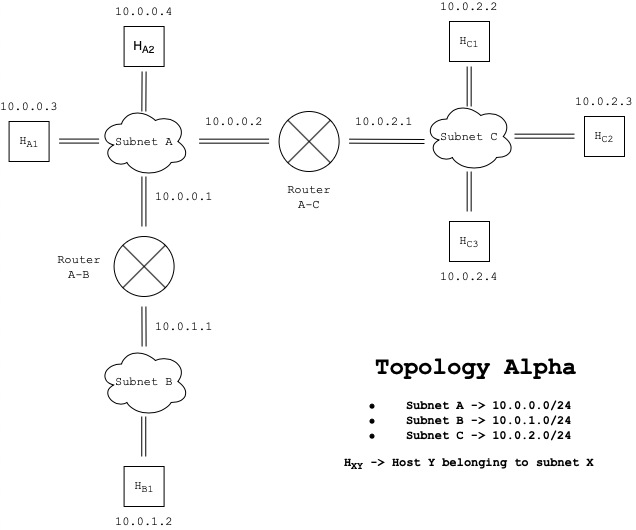
\includegraphics[width=0.75\linewidth]{topology_alpha.png}
                \caption{The \textit{Alpha Topology}.}
                \label{fig:top-alpha}
            \end{figure}

        \subsection{Topology Beta}
            This second topology added another subnetwork to the previous to push our routing procedures a little further. It is shown on figure \ref{fig:top-beta}.\\

            \begin{figure}
                \centering
                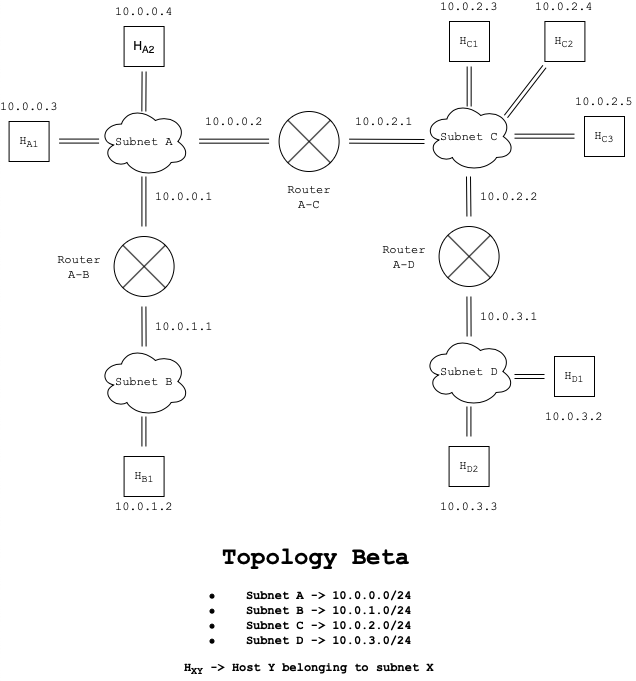
\includegraphics[width=0.75\linewidth]{topology_beta.png}
                \caption{The \textit{Beta Topology}.}
                \label{fig:top-beta}
            \end{figure}

        \subsection{Topology Gamma}
            This third topology added yet another subnetwork to the previous one. After successfully instantiating this topology we felt confident our design was capable of handling significantly more complex topologies. It is shown on figure \ref{fig:top-gamma}.\\

            \begin{figure}
                \centering
                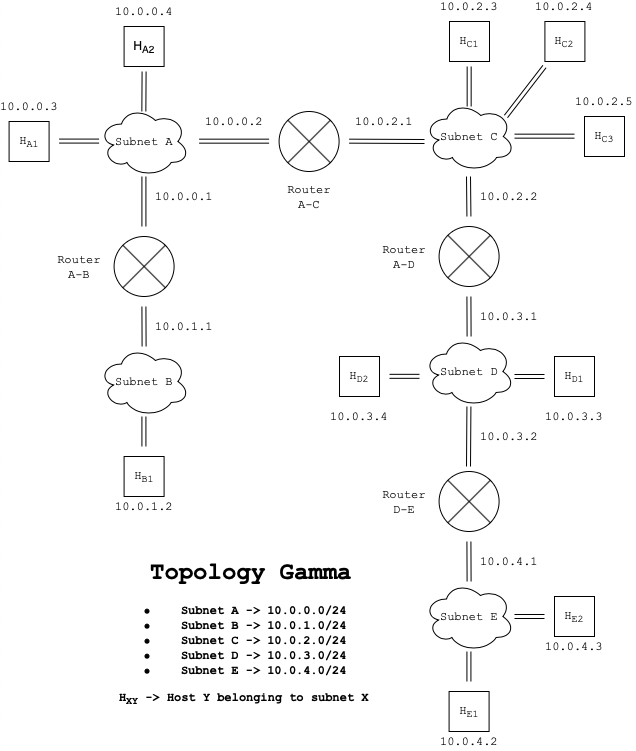
\includegraphics[width=0.75\linewidth]{topology_gamma.png}
                \caption{The \textit{Gamma Topology}.}
                \label{fig:top-gamma}
            \end{figure}

        \subsection{Topology ICS}
            This fourth topology is modeled after \textit{figure 4} of \cite{bib:ics-article}. It is the most complex one we have worked with and the one we have carried out or proof of concept on. We would like to note how, unless otherwise specified \textbf{all the firewalls drop packets}. That is, only hosts listed on the \textit{FW Conf} sections on figure \ref{fig:top-ics} are able to communicate. This topology is portrayed on figure \ref{fig:top-ics}.\\

            \begin{figure}
                \centering
                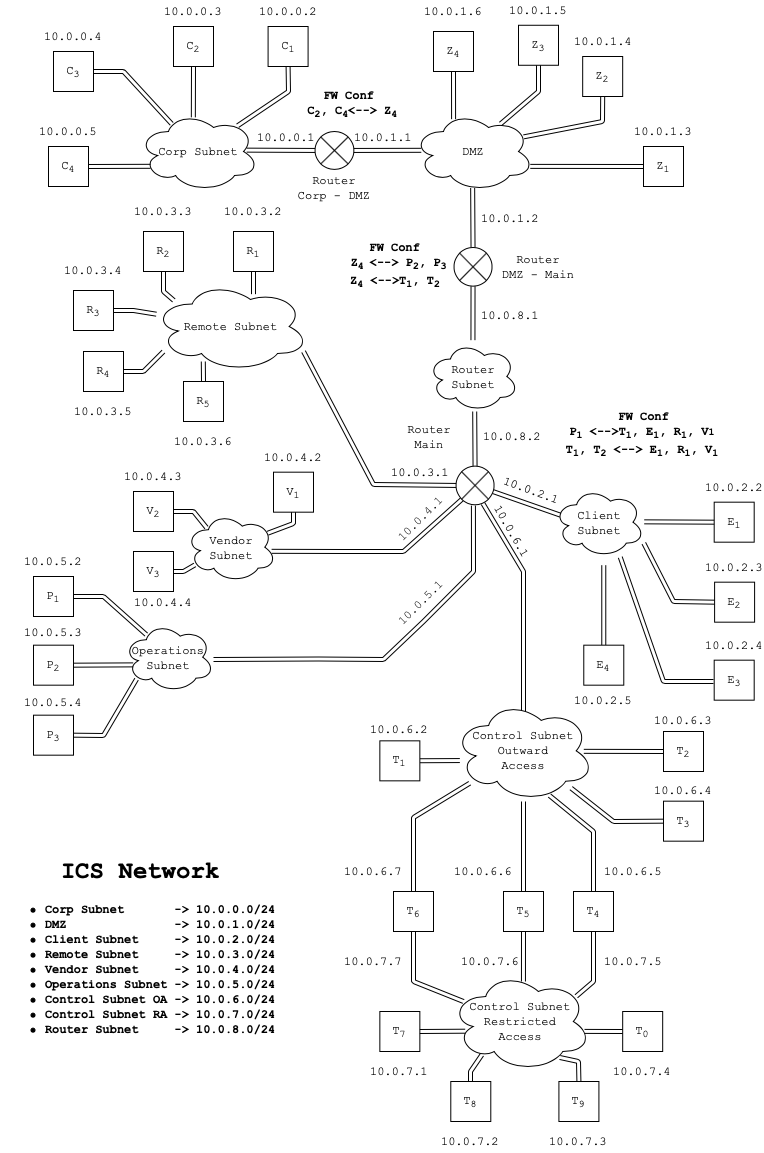
\includegraphics[width=0.75\linewidth]{topology_ics.png}
                \caption{The \textit{ICS (Industrial Control System) Topology}.}
                \label{fig:top-ics}
            \end{figure}

        \chapter{Proof of Concept}
    \section{Description}
    \section{Running the Proof of Concept}
    \section{Results}

        \chapter{Project Budget and Schedule}
    \section{Project Schedule}
        The \textit{Gantt Diagram} found on figure \ref{fig:gantt} summarizes the different periods the development process has traversed. We would like to point out that each week is assumed to last $20\ hours$, which brings the project's total duration up to $320\ hours$.
        \begin{figure}
            \centering
            \begin{tikzpicture}
                \begin{ganttchart}[
                    hgrid,
                    vgrid,
                    % y unit chart=.73cm,
                    bar/.append style={fill=cyan!50},
                    % expand chart=\linewidth
                ]{1}{16}
                    \gantttitle{Weeks}{16}\\
                    \gantttitlelist{1,...,16}{1}\\
                    \ganttbar{Information Gathering}{1}{4}\\
                    \ganttbar{Technology Assessment}{1}{4}\\
                    \ganttbar{Planning}{5}{5}\\
                    \ganttbar{Development Environment Setup}{5}{5}\\
                    \ganttbar{Development}{5}{13}\\
                    \ganttbar{Report Preparation}{13}{16}
                \end{ganttchart}
            \end{tikzpicture}
            \caption{Project's Development Phases Over Time}
            \label{fig:gantt}
        \end{figure}

    \section{Budget}
        Like in any other profession, a developer needs a set of tools to carry out his or her work in an effective manner. These incur into expenses we are detailing in this section.

        \subsection{Software Costs}
            We have strived to use only cost-free software in our development. That is why we have incurred in \textbf{no} software related costs.

        \subsection{Hardware Costs}
            Given we are working with virtual infrastructure we only need to account for the cost of our workstation when it comes to budgeting. We have developed the project with the help of a \textit{MacBook Pro} computer sporting a \textit{4 Core Intel i5 CPU at 1,4 GHz} and a \textit{16 GB RAM}. Given we have found the machine's trackpad incredibly comfortable we have not had to acquire any external accessories such as a mouse or external keyboard. The computer's cost was $1200\ \text{\euro{}}$.

        When accounting for fixed expenses such as the cost of electricity and internet access, and factoring in the regular salary for an undergrad engineer we obtain a complete budget as the one included on table \ref{tab:budget}.

        \begin{table}
            \centering
            \begin{tabular}{|c|c|c|c|}
                \hline
                \textbf{Concept} & \textbf{Units} & \textbf{Unit Cost} & \textbf{Total Cost (VAT Included)}\\
                \hline
                Software & $0$ & $0\ \text{\euro{}}$ & $0\ \text{\euro{}}$\\
                \hline
                Hardware & $1$ & $1200\ \text{\euro{}}$ & $1200\ \text{\euro{}}$\\
                \hline
                Fixed Expenses per Week & $16$ & $20\ \text{\euro{}}$ & $320\ \text{\euro{}}$\\
                \hline
                Salary per hour & $320$ & $10\ \text{\euro{}}$ & $3200\ \text{\euro{}}$\\
                \hline
            \end{tabular}
            \caption{Project's Budget}
            \label{tab:budget}
        \end{table}


    % Appendixes
        % No kidding: https://dictionary.cambridge.org/dictionary/english/appendix)
        \appendix
        \chapter{Project Budget and Schedule}
    \section{Project Schedule}
        The \textit{Gantt Diagram} found on figure \ref{fig:gantt} summarizes the different periods the development process has traversed. We would like to point out that each week is assumed to last $20\ hours$, which brings the project's total duration up to $320\ hours$.
        \begin{figure}
            \centering
            \begin{tikzpicture}
                \begin{ganttchart}[
                    hgrid,
                    vgrid,
                    % y unit chart=.73cm,
                    bar/.append style={fill=cyan!50},
                    % expand chart=\linewidth
                ]{1}{16}
                    \gantttitle{Weeks}{16}\\
                    \gantttitlelist{1,...,16}{1}\\
                    \ganttbar{Information Gathering}{1}{4}\\
                    \ganttbar{Technology Assessment}{1}{4}\\
                    \ganttbar{Planning}{5}{5}\\
                    \ganttbar{Development Environment Setup}{5}{5}\\
                    \ganttbar{Development}{5}{13}\\
                    \ganttbar{Report Preparation}{13}{16}
                \end{ganttchart}
            \end{tikzpicture}
            \caption{Project's Development Phases Over Time}
            \label{fig:gantt}
        \end{figure}

    \section{Budget}
        Like in any other profession, a developer needs a set of tools to carry out his or her work in an effective manner. These incur into expenses we are detailing in this section.

        \subsection{Software Costs}
            We have strived to use only cost-free software in our development. That is why we have incurred in \textbf{no} software related costs.

        \subsection{Hardware Costs}
            Given we are working with virtual infrastructure we only need to account for the cost of our workstation when it comes to budgeting. We have developed the project with the help of a \textit{MacBook Pro} computer sporting a \textit{4 Core Intel i5 CPU at 1,4 GHz} and a \textit{16 GB RAM}. Given we have found the machine's trackpad incredibly comfortable we have not had to acquire any external accessories such as a mouse or external keyboard. The computer's cost was $1200\ \text{\euro{}}$.

        When accounting for fixed expenses such as the cost of electricity and internet access, and factoring in the regular salary for an undergrad engineer we obtain a complete budget as the one included on table \ref{tab:budget}.

        \begin{table}
            \centering
            \begin{tabular}{|c|c|c|c|}
                \hline
                \textbf{Concept} & \textbf{Units} & \textbf{Unit Cost} & \textbf{Total Cost (VAT Included)}\\
                \hline
                Software & $0$ & $0\ \text{\euro{}}$ & $0\ \text{\euro{}}$\\
                \hline
                Hardware & $1$ & $1200\ \text{\euro{}}$ & $1200\ \text{\euro{}}$\\
                \hline
                Fixed Expenses per Week & $16$ & $20\ \text{\euro{}}$ & $320\ \text{\euro{}}$\\
                \hline
                Salary per hour & $320$ & $10\ \text{\euro{}}$ & $3200\ \text{\euro{}}$\\
                \hline
            \end{tabular}
            \caption{Project's Budget}
            \label{tab:budget}
        \end{table}

        \chapter{System Setup}
    One of the main aspects we sought when designing the project was making the installation procedure as simple as possible. The following sections describe how to install and configure all the necessary tools. We will assume the target system is running a \textit{Debian-based} distribution. If that is not the case, we encourage the reader to query his or her distribution's documentation to find out what package manager to use instead of \textit{apt}. Common examples are \textit{dnf} and \textit{pacman} for \textit{Fedora} and \textit{Arch-based} distributions, respectively. Some package names might slightly differ as well: beware.\\

    \section{Installing External Dependencies}
        We will describe how one can check whether the necessary tools are present or not. After that, we include listing \ref{lst:dependency-installation}, which contains the necessary commands to install each of the components in case they are not already present. Note several of the commands contain a leading \textit{sudo} to signify they will require elevated privileges. This might however not be needed in case it is \textit{root} him or herself who is running these commands.\\

        \subsection{iproute2}
            This project \textbf{requires} a machine running the \textit{linux kernel}. Most modern linux distributions will ship with the \textit{iproute2} suite preinstalled, but if that is not the case it needs to be installed. In order to determine whether \textit{iproute2} is available one can run \texttt{which ip}. If the command's output is \textbf{not} empty, the necessary tools are present.\\

        \subsection{Docker}
            Once can run \texttt{docker --version} to determine whether it is present on the system or not. We are including the necessary commands to acquire it on listing \ref{lst:dependency-installation}, but we encourage the reader to visit \cite{bib:docker-install} as it contains a more comprehensive explanation on the process.\\

        \subsection{PIP}
            \textit{PIP} is \textit{python's} package manager. Running \texttt{\allowbreak python3 -m pip --version} aides in determining whether it is present on the system or not. If it is, a message containing information on \textit{PIP's} version will be printed.\\

        \subsection{Python Modules}
            Our tool depends on both the \textit{matplotlib} and \textit{networkx} modules. Once \textit{PIP} is installed on the system we can run \texttt{\allowbreak python3 -m pip list | grep <module-name>} to determine whether module \textit{<module-name>} is present on the system or not. If the previous command shows no output, the specified module is not present on the system. Note listing \ref{lst:dependency-installation} explicitly uses \textit{sudo} when installing these modules. We delve a little deeper into that fact in a later section.\\

        \begin{lstlisting}[language = bash, caption = Commands for installing needed dependencies., label = lst:dependency-installation]
            # If any packages are to be installed with apt,
                # update the repositories.
            sudo apt update

            # Installing iproute2
            sudo apt install iproute2

            # Installing docker
                # Auxiliary packages
                sudo apt install \
                    apt-transport-https \
                    ca-certificates \
                    curl \
                    gnupg \
                    lsb-release

                # Obtaining Docker's repository GPG key
                curl -fsSL https://download.docker.com/linux/ubuntu/gpg \
                    | sudo gpg --dearmor -o \
                    /usr/share/keyrings/docker-archive-keyring.gpg

                # Adding Docker's repository to the system
                echo \
                    "deb [arch=amd64 signed-by=/usr/share/keyrings/ \
                        docker-archive-keyring.gpg] https://download \
                        .docker.com/linux/ubuntu $(lsb_release -cs) \
                        stable" | sudo tee /etc/apt/sources.list.d/ \
                        docker.list > /dev/null

                # Updating the repositories
                sudo apt update

                # Installing docker itself
                sudo apt install docker-ce docker-ce-cli containerd.io

            # Installing PIP
            sudo apt install python3-pip

            # Installing python modules matplotlib and networkx
                # Note the can be installed separately.
            sudo python3 -m pip install matplotlib networkx
        \end{lstlisting}

    \section{A note on Capabilities}
        On section \ref{sec:user-manual} we already introduced the term \textit{capability}. As seen on \cite{bib:man-capabilities}, \textit{capabilities} allow for a finer control so as to what a process can and cannot do. What is more, a process spawned by a non-privileged user can take actions traditionally reserved for those started by a privileged user as long as it is granted the necessary capabilities. The reader might recall listing \ref{lst:running-nodes} in which we were explicitly assigning several capabilities to the containers we were spawning so that they could perform several needed actions. One of the benefits of using containers is that they allow for a tighter control on what the process running within them can and cannot do. That is why they do are not granted all the capabilities by default.\\

        Capabilities are a feature of the linux kernel, and thus they can be applied to other scenarios. One of the conditions for running our program set forth in section \ref{sec:user-manual} was that it needed to be executed as \textit{root}. The limitation was imposed by the need to leverage the \textit{iproute2} suite for the configuration of the network interfaces associated to the containers. Now, if we apply the concept of capabilities to this particular case we can free ourselves from such a limitation. Given we are passing strings to the \texttt{os.system()} function we are exposing the host to injection attacks through, for example, malicious node names. Listing \ref{lst:injection-atk} contains one such example.\\

        A key piece of information extracted from \cite{bib:man-capabilities} is shown on listing \ref{lst:exec-caps}. It shows how the capabilities of a process are transformed when a call to \texttt{execve()} \cite{bib:man-execve} takes place. Given how shells such as \textit{bash} \cite{bib:man-bash} work, they rely on \texttt{execve()} for launching other programs, which implies the rules set forth on listing \ref{lst:exec-caps} are of the utmost importance.\\

        \begin{lstlisting}[language = {}, caption = Transformation of Capabilities During \texttt{execve()}., label = lst:exec-caps]
            P'(ambient)     = (file is privileged) ? 0 : P(ambient)
            P'(permitted)   = (P(inheritable) & F(inheritable)) |
                                (F(permitted) & P(bounding)) | P'(ambient)
            P'(effective)   = F(effective) ? P'(permitted) : P'(ambient)
            P'(inheritable) = P(inheritable)    [i.e., unchanged]
            P'(bounding)    = P(bounding)       [i.e., unchanged]
            where:
                P()       denotes the value of a thread capability set before
                              the execve(2)
                P'()      denotes the value of a thread capability set after
                              the execve(2)
                F()       denotes a file capability set
                &         denotes the AND logical operation between sets.
                |         denotes the OR logical operation between sets.
                A ? B : C denotes an IF-ELSE close that can be read as: if
                              A is TRUE then B ELSE C.
        \end{lstlisting}

        Given the contents of listing \ref{lst:exec-caps} one might feel overwhelmed. The key idea is to somehow make sure that the processes effective set (i.e. \texttt{P'(effective)}) contains the capabilities we want to grant. In our case we seek granting the \textit{CAP\_NET\_ADMIN} capability to the host's \textit{iproute2} binary. This would imply that we would no longer need to run our program as \texttt{root} \footnote{Disabling the calls to \textit{iptables} as discussed on section \ref{sec:bridge-caveats} would still require privileges. This can nonetheless be done manually without impacting the tool's main use.}, thus denying a huge attack vector.\\

        We must begin by locating the \texttt{ip} binary within the system. This can easily be accomplished by running \texttt{\allowbreak readlink \$(which ip)}. This command will either show the real path to the \texttt{ip} or show no output. In the latter case, the binary's real path is given by \texttt{which ip}. In our case on a machine running \textit{Ubuntu 20.04} \texttt{which ip} returns \texttt{/usr/sbin/ip} which is a symbolic link to \texttt{/bin/ip}, the real executable.\\

        Now that we have located the program itself we need to make sure that \textit{CAP\_NET\_ADMIN} makes its way to the \texttt{P'(effective)} set. This implies the \textit{effective} (i.e. \texttt{F(effective)}) flag must be set for \texttt{/bin/ip} and that \textit{CAP\_NET\_ADMIN} should belong to \texttt{P'(permitted)}. In order for this to be true, the \textit{CAP\_NET\_ADMIN} capability must belong to the file's \textit{permitted} (i.e. \texttt{F(permitted)}) set and the same capability must belong to the \texttt{P(bounding)} set.\\

        These changes can be made effective through the \texttt{setcap} \cite{bib:man-setcap} command. Running \texttt{sudo setcap cap\_net\_admin+ep /bin/ip} does indeed configure the capabilities as shown by the output of \texttt{getcap /bin/ip} \cite{bib:man-getcap}. On top of that, we can leverage the \texttt{capsh --print} \cite{bib:man-capsh} command to query the current process' (i.e. the \textit{shell's}) \textit{bounding} capabilities (i.e. \texttt{P(bounding)}) to indeed check that \textit{CAP\_NET\_ADMIN} belongs to it. To the extent of what we know this would need to be sufficient to be able to leverage \texttt{ip} to carry out network-related tasks. To our uttermost surprise, it was not.\\

        If one browses \textit{iproute2's} source code on \cite{bib:iproute2-src} line $181$ on file \textit{iproute2/ip/ip.c} \footnote{\url{https://github.com/shemminger/iproute2/blob/main/ip/ip.c\#L181}} has a suspicious looking name. The definition of the \texttt{drop\_cap()} function called on it is found on lines $1571 \to 1597$ of file \textit{iproute2/lib/utils.c} \footnote{\url{https://github.com/shemminger/iproute2/blob/main/lib/utils.c\#L1571-L1597}} and is included on listing \ref{lst:drop-cap} for convenience. The key aspect to note is that the function checks whether the \textit{CAP\_NET\_ADMIN} capability belongs to the process' \textit{inheritable} set (i.e. \texttt{P'(inheritable)}) as we have already \texttt{execve()}ed from the shell. Given this set remains unchanged, we can rest assured \texttt{ip} is effectively checking whether the \textit{CAP\_NET\_ADMIN} capability belonged to the shell's \textit{inheritable} set (i.e. \texttt{P(inheritable)}). As that was \textbf{not} the case (we had not modified the shell's binary) then the check on line $18$ of listing \ref{lst:drop-cap} evaluates to \texttt{true == 1}, which makes makes \texttt{ip} drop \textbf{all} the capabilities we have explicitly provided through \texttt{setcap}.\\

        \lstinputlisting[language = c, caption = Defintion of the \texttt{drop\_cap()} Function., label = lst:drop-cap]{Code_snippets/drop_cap.c}

        The check on line $18$ opens up a door for executing \texttt{ip} with the aid of capabilities. When we read the \texttt{drop\_cap()} function we began wondering the motivation behind it. Given our approach of adding the \textit{CAP\_NET\_ADMIN} capability to both the \textit{effective} and \textit{permitted} sets for \texttt{/bin/ip}, we are effectively allowing any user modify the machine's network configuration. This poses a potential security risk. In our quest for a solution to this limitation we encountered a solution that circumvents this issue whilst allowing a more fine grained approach to the management of capabilities.\\

    \section{Acquiring the Project's Code}
        \subsection{Leveraging \texttt{git}}
            \subsubsection{Cloning the Repository}
            \subsubsection{Proposing Changes}
    \section{Framework Code}
        \chapter{Comprehensive Module Analysis}
    \section{The virt\_net Module} \label{sec:virt-net-module}
        \subsubsection{Constants.py}
    In an effort to reduce the number of dependencies we decided to leverage \textit{ANSI Escape Codes} to colour the different output messages. This module then defines the different \texttt{strings} controlling the colours.

    \paragraph{Imported Libraries}
        None as there are no external dependencies.

    \paragraph{Global Variables}
        \begin{enumerate}
            \item \textbf{\texttt{terminal\_escape\_sequences (dictionary/string/string)}:} \texttt{Dictionary} keyed by color names whose associated values are \texttt{ANSI Escape Sequences} changing the terminal's output color to the one specified. This solution is \textbf{not} to be considered portable. It \textbf{should} nonetheless work on any regular terminals supporting colors. We can assure it works with the following terminal emulators: \texttt{tilix}, \texttt{kitty} and \texttt{Visual Studio Code's Embedded Terminal Emulator}.
        \end{enumerate}
        \subsubsection{Interface.py}
    This class will be in charge of providing a node's network functionality. An interface represents a connection with a computer network and thus is defined by a key parameter: the IP address. We should stress how an IP address is associated with an interface, \textbf{not} with the host itself. This subtlety will be extremely relevant when dealing with routers.\\

    Another key aspect of interfaces is the role they play in network routes. Even though it is not entirely correct, in our case we can talk about the interface's routes. If we are being precise we would consider routes to be associated to a machine's network stack, not to a given interface. Nonetheless, as the graphs we are to instantiate will always define topologies in such a way that only an interface per host will belong to a given subnet we can indeed associate a route with an interface for a given route will only egress through a specific interface. This distinction will allow us to quickly and univocally query a node's route configuration.\\

    Once an interface is configured it will just support a machine's connections. It is also crucial to note that even though an instance of the \texttt{interface} class is \textbf{not} the same thing as a \texttt{veth}, they are intimately related. Instantiating an \texttt{interface} will trigger the creation of a \texttt{veth} and deleting the former will also remove the latter. All in all, an interface's lifecycle can be described as:\\

    \begin{enumerate}
        \item An interface instance is created and the associated \texttt{veth} is created as well.
        \item The interface is assigned an IP address.
        \item One or more routes are assigned to or deleted from the interface.
        \item The interface sits idle until it returns to $2$ or $3$ or goes to $5$.
        \item The interface is removed, which will also remove the corresponding \texttt{veth}.
    \end{enumerate}

    \paragraph{Imported Libraries}
        \begin{enumerate}
            \item \textbf{\texttt{os}:} This module enables the execution of commands through a \texttt{sh} shell through the \texttt{os.system()} method. One can check the shell being spawned is indeed \texttt{sh} by running \texttt{\allowbreak os.system("echo \$0")} or by querying \cite{bib:man-system}.
            \item \textbf{\texttt{constants}:} Grant access to the \texttt{\allowbreak terminal\_escape \_sequences dictionary} containing \texttt{ANSI escape sequences} enabling colored output.
        \end{enumerate}

    \paragraph{Global Variables}
        \begin{enumerate}
            \item \textbf{\texttt{\allowbreak t\_colors - dictionary/string/string}:} This is a synonym for the \texttt{\allowbreak terminal\_esc ape\_sequences dictionary} we me mentioned before. It is used within calls to \texttt{print()} so that we can alter the terminal text's color allowing for a more visual information representation.
        \end{enumerate}

    \paragraph{The \texttt{interface} Class}
        This class represents a host's interface.

        \subparagraph{Class Attributes}
            \begin{enumerate}
                \item \textbf{\texttt{self.host\_name - string}:} Name identifying the host this interface belongs to.
                \item \textbf{\texttt{self.ip\_range - string}:} Interface's IP and subnet mask in \textit{CIDR} \cite{bib:cidr-notation} format. Ex: \texttt{"10.0.0.1/24"}.
                \item \textbf{\texttt{self.ip - string}:} Interface's IP address.
                \item \textbf{\texttt{self.if\_name - string}:} Interface's name. This is equivalent to traditional names like \texttt{enp2s0} or \texttt{wlp3s0} in Linux-based systems. In our case the names will follow a pattern given by \texttt{veth\_+\_-} where \texttt{+} and \texttt{-} are the names of the connected nodes. Note either \texttt{+} or \texttt{-} will be the same as \texttt{self.host\_name}. We would finally like to point out that \texttt{+} and \texttt{-} can be either upper or lowercase, depending on which is the first node to be attached to the links we create.
                \item \textbf{\texttt{self.subn\_gateway - string}:} IP address of this subnet's gateway, following the same format as \texttt{self.ip}.
                \item \textbf{\texttt{self.subn - string}:} Interface's subnet given as the network address for said subnet together with the subnet mask in \texttt{CIDR} notation. Ex: \texttt{10.0.0.0/24}.
                \item \textbf{\texttt{self.outbound\_interface - boolean}:} \texttt{True} if the interface's host is allowed to connect to external subnets. \texttt{False} otherwise. Due to how some ICS networks need to isolate some equipment, such as reactor's control systems, we need to know whether a given host is allowed to ``see'' the outside world. Having this information encoded into interfaces allows for a cleaner design when routing the network.
            \end{enumerate}

        \subparagraph{The \texttt{Constructor}}
            \begin{enumerate}
                \item \textbf{Parameters:}
                \begin{enumerate}
                    \item \texttt{self - interface\_inst:} The actual interface instance.
                    \item \texttt{h\_name - string:} The host the interface belongs to.
                    \item \texttt{if\_name - string:} The interface name
                    \item \texttt{subnet - string:} The subnet the interface belongs to.
                    \item \texttt{h\_type - boolean:} \texttt{True} if the interface belongs to a regular node, \texttt{False} otherwise.
                    \item \texttt{out\_interface - boolean - optional:} \texttt{True} if the node is allowed to ``see'' other subnets, \texttt{False} otherwise.
                \end{enumerate}
                \item \textbf{Returns:} Nothing.
                \item \textbf{Description:} This method will initialize the members of an \texttt{interface\_inst} and call the \texttt{\_activate\_iface()} method.
            \end{enumerate}

        \subparagraph{The \texttt{\_activate\_iface()} Method}
            \begin{enumerate}
                \item \textbf{Parameters:}
                \begin{enumerate}
                    \item \texttt{self - interface\_inst:} The actual interface instance.
                \end{enumerate}
                \item \textbf{Returns:} Nothing.
                \item \textbf{Description:} This method leverages the \texttt{os.system()} function to activate a \texttt{veth} interface. The \texttt{string} we pass \texttt{os.system()} is built though the concatenation of several instance attributes. As we usually do, we check whether \texttt{os.system()}'s return code was $0$ to show an informative message to the user.
            \end{enumerate}

        \subparagraph{The \texttt{get\_if\_subnet()} Method}
            \begin{enumerate}
                \item \textbf{Parameters:}
                \begin{enumerate}
                    \item \texttt{self - interface\_inst:} The actual interface instance.
                \end{enumerate}
                \item \textbf{Returns:} A \texttt{string} containing the subnet the interface belongs to in \texttt{CIDR} notation.
                \item \textbf{Description:} Not applicable.
            \end{enumerate}

        \subparagraph{The \texttt{get\_if\_ip\_range()} Method}
            \begin{enumerate}
                \item \textbf{Parameters:}
                \begin{enumerate}
                    \item \texttt{self - interface\_inst:} The actual interface instance.
                \end{enumerate}
                \item \textbf{Returns:} A \texttt{string} containing the interface's IP and subnet mask in \texttt{CIDR} format.
                \item \textbf{Description:} Not applicable.
            \end{enumerate}

        \subparagraph{The \texttt{get\_if\_ip()} Method}
            \begin{enumerate}
                \item \textbf{Parameters:}
                \begin{enumerate}
                    \item \texttt{self - interface\_inst:} The actual interface instance.
                \end{enumerate}
                \item \textbf{Returns:} A \texttt{string} containing the interface's IP.
                \item \textbf{Description:} Not applicable.
            \end{enumerate}

        \subparagraph{The \texttt{get\_if\_name()} Method}
            \begin{enumerate}
                \item \textbf{Parameters:}
                \begin{enumerate}
                    \item \texttt{self - interface\_inst:} The actual interface instance.
                \end{enumerate}
                \item \textbf{Returns:} A \texttt{string} containing the interface's name.
                \item \textbf{Description:} Not applicable.
            \end{enumerate}

        \subparagraph{The \texttt{get\_routes()} Method}
            \begin{enumerate}
                \item \textbf{Parameters:}
                \begin{enumerate}
                    \item \texttt{self - interface\_inst:} The actual interface instance.
                \end{enumerate}
                \item \textbf{Returns:} A \texttt{dictionary/string/string} containing the routes that have been assigned through this interface.
                \item \textbf{Description:} Not applicable.
            \end{enumerate}

        \subparagraph{The \texttt{set\_if\_name()} Method}
            \begin{enumerate}
                \item \textbf{Parameters:}
                \begin{enumerate}
                    \item \texttt{self - interface\_inst:} The actual interface instance.
                    \item \texttt{if\_name - string}
                \end{enumerate}
                \item \textbf{Returns:} Nothing.
                \item \textbf{Description:} Assigns the value of the \texttt{if\_name} parameter to the \texttt{self.if\_name} attribute.
            \end{enumerate}

        \subparagraph{The \texttt{assign\_addr()} Method}
            \begin{enumerate}
                \item \textbf{Parameters:}
                \begin{enumerate}
                    \item \texttt{self - interface\_inst:} The actual interface instance.
                    \item \texttt{ip\_range - string:} The interface's IP address together with its subnet mask.
                    \item \texttt{gw\_addr - string - optional:} IP address of the subnet's gateway (i.e. router).
                    \item \texttt{subnet - string - optional:} The subnet the interface belongs to in \texttt{CIDR} format.
                \end{enumerate}
                \item \textbf{Returns:} Nothing.
                \item \textbf{Description:} This method lets the caller assign an IP address to the interface. The method will check that the interface name is valid and that the interface had no previous address to avoid errors. Note that when a node moves within the network its interface \textbf{will not} be reconfigured: a new one will be added to the node. Once the addressing has been successfully completed a message stating that will be printed.
            \end{enumerate}

        \subparagraph{The \texttt{assign\_route()} Method}
            \begin{enumerate}
                \item \textbf{Parameters:}
                \begin{enumerate}
                    \item \texttt{self - interface\_inst:} The actual interface instance.
                    \item \texttt{dest\_subnet - string:} Destination subnet for the route in \texttt{CIDR} format.
                    \item \texttt{gw\_router - string:} IP of the gateway for the interface's subnet.
                \end{enumerate}
                \item \textbf{Returns:} Nothing.
                \item \textbf{Description:} After checking the interface has been assigned an IP address and that it is allowed to communicate with other subnets through the \texttt{self.outbound\_inter face} attribute it will add the route defined by the parameters to the \texttt{self.routes dictionary}.
            \end{enumerate}

        \subparagraph{The \texttt{reset\_interface()} Method}
            \begin{enumerate}
                \item \textbf{Parameters:}
                \begin{enumerate}
                    \item \texttt{self - interface\_inst:} The actual interface instance.
                \end{enumerate}
                \item \textbf{Returns:} Nothing.
                \item \textbf{Description:} This method will wipe the \texttt{self.routes dictionary} and remove the interface's IP address. This will also delete any preexisting routes. As usual, an informative message will inform of the operation's success.
            \end{enumerate}

        \subparagraph{The \texttt{remove\_interface()} Method}
            \begin{enumerate}
                \item \textbf{Parameters:}
                \begin{enumerate}
                    \item \texttt{self - interface\_inst:} The actual interface instance.
                \end{enumerate}
                \item \textbf{Returns:} Nothing.
                \item \textbf{Description:} This method will delete the associated interface, together with all the routes, and print an informative message upon completion.
            \end{enumerate}

        \subparagraph{The \texttt{Destructor}}
            \begin{enumerate}
                \item \textbf{Parameters:}
                \begin{enumerate}
                    \item \texttt{self - interface\_inst:} The actual interface instance.
                \end{enumerate}
                \item \textbf{Returns:} Nothing.
                \item \textbf{Description:} This method will just call \texttt{remove\_interface()}.
            \end{enumerate}
        \subsubsection{\texttt{Subnet\_Machines.py}}
    This file contains the class definitions for the elements belonging to a subnetwork: \texttt{bridges} and \texttt{nodes}. We would like to clarify that we refer to regular \texttt{hosts} as \texttt{nodes} interchangeably.\\

    We have purposefully decided \textbf{not to consider} \texttt{routers} as part of these subnetworks. The logic behind the decision is that a \texttt{router} belongs to at least two subnetworks in out topologies. Thus, defining its class in a file whose context is that of a single subnetwork did not seem appropriate.\\

    Once again, we should point out how an instance of the \texttt{k\_bridge} class \textbf{is not} the same thing as the actual \texttt{bridge}, but they are intimately related. The following explains the lifecycle of both classes defined in this file.\\

    \begin{enumerate}
        \item The real instance, either a \texttt{bridge} or a \texttt{host}, is brought up.
        \item The object representing said instance is created.
        \item The object sits idle. Several of its parameters can be altered within this state.
        \item At some point, the object will be dismantled.
        \item The release of the object will trigger the removal of the associated real instance.
    \end{enumerate}

    \paragraph{Imported Libraries}
        \begin{enumerate}
            \item \textbf{\texttt{os}:} This module enables the execution of commands through a \texttt{sh} shell through the \texttt{os.system()} method. One can check the shell being spawned is indeed \texttt{sh} by running \texttt{\allowbreak os.system("echo \$0")} or bu querying the following \href{https://linux.die.net/man/3/system}{\texttt{manpage}}.
            \item \textbf{\texttt{constants}:} Grant access to the \texttt{\allowbreak terminal\_escape\_sequences dictionary} containing \texttt{ANSI escape sequences} enabling colored output.
            \item \textbf{\texttt{sys}:} This module allows us to print error messages to \texttt{STDERR} instead of \texttt{STDOUT} so that they can be easily redirected later on if needed with \texttt{2>/path/to/log}.
            \item \textbf{\texttt{subprocess}:} This module enables the execution of commands through a shell \textbf{and} allows the caller to retrieve the command's output to \texttt{STDOUT} on top of its return code. This will let us retrieve a container's associated \texttt{PID}.
            \item \textbf{\texttt{interface}:} This module will let us instantiate and add \texttt{interface\_inst} to the nodes we create.
        \end{enumerate}

    \paragraph{Global Variables}
        \begin{enumerate}
            \item \textbf{\texttt{\allowbreak t\_colors - dictionary/string/string}:} This is a synonym for the \texttt{\allowbreak terminal\_escape\_sequences dictionary} we me mentioned before. It is used within calls to \texttt{print()} so that we can alter the terminal text's color allowing for a more visual information representation.
        \end{enumerate}

    \paragraph{The \texttt{k\_bridge} Class}
        This class represents a virtual bridge. Note the \texttt{k} stands for kernel as these bridges are part of the kernel itself.

        \subparagraph{Class Attributes}
            \begin{enumerate}
                \item \textbf{\texttt{self.type - string}:} Object type identifier containing the \texttt{"bridge" string} for bridges. It is used within functions to check the type of object it is currently dealing with.
                \item \textbf{\texttt{self.name - string}:} Bridge's name.
                \item \textbf{\texttt{self.up - boolean}:} \texttt{True} if the bridge is currently up (i.e. ``switched on''). \texttt{False} otherwise.
                \item \textbf{\texttt{self.subnet - string}:} Bridge's associated subnetwork given as the network address for said subnetwork together with the subnet mask in \texttt{CIDR} notation.
            \end{enumerate}

        \subparagraph{The \texttt{Constructor}}
            \begin{enumerate}
                \item \textbf{Parameters:}
                \begin{enumerate}
                    \item \texttt{self - k\_birdge\_inst:} The actual bridge instance.
                    \item \texttt{name - string:} The bridge's name.
                    \item \texttt{subnet - string:} The subnetwork associated with this bridge.
                \end{enumerate}
                \item \textbf{Returns:} Nothing.
                \item \textbf{Description:} This method will initialize the members of an \texttt{k\_bridge\_inst} and call the \texttt{\_activate\_bridge()} method.
            \end{enumerate}

        \subparagraph{The \texttt{\_activate\_bridge()} Method}
            \begin{enumerate}
                \item \textbf{Parameters:}
                \begin{enumerate}
                    \item \texttt{self - k\_bridge\_inst:} The actual bridge instance.
                \end{enumerate}
                \item \textbf{Returns:} Nothing.
                \item \textbf{Description:} After the bridge has been instantiated it must be brought up so that it can be operated normally. We do so through the \texttt{ip link} command, printing a message on success. Once the bridge is activated, the \texttt{self.up} attribute will be set to \texttt{True}.
            \end{enumerate}

        \subparagraph{The \texttt{get\_name()} Method}
            \begin{enumerate}
                \item \textbf{Parameters:}
                \begin{enumerate}
                    \item \texttt{self - k\_bridge\_inst:} The actual bridge instance.
                \end{enumerate}
                \item \textbf{Returns:} A \texttt{string} containing the bridge's name.
                \item \textbf{Description:} Not applicable.
            \end{enumerate}

        \subparagraph{The \texttt{get\_type()} Method}
            \begin{enumerate}
                \item \textbf{Parameters:}
                \begin{enumerate}
                    \item \texttt{self - k\_bridge\_inst:} The actual bridge instance.
                \end{enumerate}
                \item \textbf{Returns:} The \texttt{"bridge" string}.
                \item \textbf{Description:} Not applicable.
            \end{enumerate}

        \subparagraph{The \texttt{get\_subnet()} Method}
            \begin{enumerate}
                \item \textbf{Parameters:}
                \begin{enumerate}
                    \item \texttt{self - k\_bridge\_inst:} The actual bridge instance.
                \end{enumerate}
                \item \textbf{Returns:} A \texttt{string} containing the bridge's associated subnet in \texttt{CIDR} format.
                \item \textbf{Description:} Not applicable.
            \end{enumerate}

        \subparagraph{The \texttt{remove()} Method}
            \begin{enumerate}
                \item \textbf{Parameters:}
                \begin{enumerate}
                    \item \texttt{self - k\_bridge\_inst:} The actual bridge instance.
                \end{enumerate}
                \item \textbf{Returns:} Nothing.
                \item \textbf{Description:} This method shuts the bridge down. It will check it is indeed activated before doing so in an effort to prevent errors provoked by calling \texttt{ip link} with incorrect parameters (i.e. such as by trying to shutdown a bridge that is already down). This method will print a message to \texttt{STDOUT} informing whether the operation was a success or not.
            \end{enumerate}

        \subparagraph{The \texttt{Destructor}}
            \begin{enumerate}
                \item \textbf{Parameters:}
                \begin{enumerate}
                    \item \texttt{self - k\_bridge\_inst:} The actual bridge instance.
                \end{enumerate}
                \item \textbf{Returns:} Nothing.
                \item \textbf{Description:} This method will just call \texttt{remove()}.
            \end{enumerate}

    \paragraph{The \texttt{d\_node} Class}
        This class represents a node implementing a virtual host. Note the \texttt{d} stands for docker.

        \subparagraph{Class Attributes}
            \begin{enumerate}
                \item \textbf{\texttt{self.type - string}:} Object type identifier containing the \texttt{"node" string} for nodes. It is used within functions to check the type of object it is currently dealing with.
                \item \textbf{\texttt{self.name - string}:} Node's name.
                \item \textbf{\texttt{self.pid - int}:} The associated container's \texttt{PID}. It is used when linking the container's network namespace to \texttt{/var/run/netns} so that we can easily access it afterwards.
                \item \textbf{\texttt{self.interfaces - list/interface\_inst}:}  A list containing the instances of the interfaces belonging to this node.
            \end{enumerate}

        \subparagraph{The \texttt{Constructor}}
            \begin{enumerate}
                \item \textbf{Parameters:}
                \begin{enumerate}
                    \item \texttt{self - d\_node\_inst:} The actual node instance.
                    \item \texttt{name - string:} The node's name.
                \end{enumerate}
                \item \textbf{Returns:} Nothing.
                \item \textbf{Description:} This method will just initialize several members with the passed parameters whilst assigning sane defaults to others. It leverages the power of the \texttt{docker inspect} command to find the associated container's \texttt{PID}. It will also call \texttt{\_link\_net\_namespace()} to allow an easier handling of the container's namespace through the \texttt{ip} command. It finally calls \texttt{\_set\_hostname()} to configure the node's identity from the network's perspective.
            \end{enumerate}

        \subparagraph{The \texttt{\_link\_net\_namespace()} Method}
            \begin{enumerate}
                \item \textbf{Parameters:}
                \begin{enumerate}
                    \item \texttt{self - d\_node\_inst:} The actual node instance.
                \end{enumerate}
                \item \textbf{Returns:} Nothing.
                \item \textbf{Description:} This method will create a symbolic link to the container's network namespace under \texttt{/var/run/netns} where the \texttt{ip} command will ``look for'' existing named namespaces. This method leverages the \texttt{self.pid} attribute that is initialized in the constructor to find the original location of the container's namespace so that it can later be linked.
            \end{enumerate}

        \subparagraph{The \texttt{\_set\_hostname()} Method}
            \begin{enumerate}
                \item \textbf{Parameters:}
                \begin{enumerate}
                    \item \texttt{self - d\_node\_inst:} The actual node instance.
                \end{enumerate}
                \item \textbf{Returns:} Nothing.
                \item \textbf{Description:} This method will just set the container's hostname. It is essential to distinguish between the container's name and its hostname. The former is an identifier that only concerns docker, whilst the latter will be the machine's identifier from the point of view of the network. This method will make the latter the same as the former. What is more, this operation made us change the underscores (\texttt{\_}) in the original node names by hyphens (\texttt{-}): the former were not allowed on network hostnames.
            \end{enumerate}

        \subparagraph{The \texttt{get\_name()} Method}
            \begin{enumerate}
                \item \textbf{Parameters:}
                \begin{enumerate}
                    \item \texttt{self - d\_node\_inst:} The actual node instance.
                \end{enumerate}
                \item \textbf{Returns:} A \texttt{string} containing the node's name.
                \item \textbf{Description:} Not applicable.
            \end{enumerate}

        \subparagraph{The \texttt{get\_type()} Method}
            \begin{enumerate}
                \item \textbf{Parameters:}
                \begin{enumerate}
                    \item \texttt{self - d\_node\_inst:} The actual node instance.
                \end{enumerate}
                \item \textbf{Returns:} The \texttt{"node" string}.
                \item \textbf{Description:} Not applicable.
            \end{enumerate}

        \subparagraph{The \texttt{get\_subnets()} Method}
            \begin{enumerate}
                \item \textbf{Parameters:}
                \begin{enumerate}
                    \item \texttt{self - d\_node\_inst:} The actual node instance.
                \end{enumerate}
                \item \textbf{Returns:} A \texttt{list/string} containing the different subnetworks this node is connected to in \texttt{CIDR} format.
                \item \textbf{Description:} This method will iterate over the \texttt{interface\_inst} contained in the \texttt{self.interfaces} attribute to then provide a list containing the subnetworks each of these \texttt{interface\_inst} belong to. Even though nodes will usually belong to a single subnetwork this method allows for a more extensible design that can accommodate for nodes belonging to different subnetworks in more complex topologies.
            \end{enumerate}

        \subparagraph{The \texttt{get\_interface()} Method}
            \begin{enumerate}
                \item \textbf{Parameters:}
                \begin{enumerate}
                    \item \texttt{self - d\_node\_inst:} The actual node instance.
                    \item \texttt{subnet - string - optional:} Specifies the subnetwork for which an associated \texttt{interface\_inst} should be returned.
                \end{enumerate}
                \item \textbf{Returns:} The following are evaluated in order.
                \begin{enumerate}
                    \item A \texttt{list/interface\_inst} if the \texttt{subnet} parameter was not specified.
                    \item An \texttt{interface\_inst} associated to the subnetwork specified in the \texttt{subnet} parameter.
                    \item \texttt{None} if there is no interface associated with the subnetwork specified through the \texttt{subnet} parameter.
                \end{enumerate}
                \item \textbf{Description:} As seen on the \textbf{returns} section, the \texttt{subnet} parameter behaves like a switch. A \texttt{list} of \texttt{interface\_inst} will be returned if it is not specified by the caller. In case it is provided, it will return either an \texttt{interface\_inst} or \texttt{None} if there is no interface associated with the specified subnetwork.
            \end{enumerate}

        \subparagraph{The \texttt{create\_interface()} Method}
            \begin{enumerate}
                \item \textbf{Parameters:}
                \begin{enumerate}
                    \item \texttt{self - d\_node\_inst:} The actual node instance.
                    \item \texttt{if\_name - string:} Name of the interface to create.
                    \item \texttt{if\_subnet - string:} Subnet associated with the interface to create.
                    \item \texttt{o\_if - boolean:} Flag indicating whether the interface to create should be allowed to ``see'' other subnetworks.
                \end{enumerate}
                \item \textbf{Returns:} Nothing.
                \item \textbf{Description:} This method will instantiate a new interface and add it to the node's \texttt{self.interfaces list}. The method's parameters will be passed directly to the \texttt{interface} class constructor.
            \end{enumerate}

        \subparagraph{The \texttt{reset\_interfaces()} Method}
            \begin{enumerate}
                \item \textbf{Parameters:}
                \begin{enumerate}
                    \item \texttt{self - d\_node\_inst:} The actual node instance.
                \end{enumerate}
                \item \textbf{Returns:} Nothing.
                \item \textbf{Description:} This method erases all the interfaces associated with the node through the \texttt{clear()} \footnote{\href{https://docs.python.org/3/tutorial/datastructures.html}{https://docs.python.org/3/tutorial/datastructures.html}} method of the \texttt{self.interfaces list}. This method will \textit{implicitly} call the destructor for each interface, thus effectively deleting the underlying \texttt{veths}.
            \end{enumerate}

        \subparagraph{The \texttt{stop()} Method}
            \begin{enumerate}
                \item \textbf{Parameters:}
                \begin{enumerate}
                    \item \texttt{self - d\_node\_inst:} The actual node instance.
                \end{enumerate}
                \item \textbf{Returns:} A \texttt{boolean} indicating whether the operation succeeded or not.
                \item \textbf{Description:} This method is in charge of stopping the instance's associated docker container. We can do so thanks to the \texttt{docker stop} command. This method leverages a redirection to \texttt{/dev/null} so that the output generated by \texttt{docker stop} does not interfere with our own. This method will print a message both upon success and error.
            \end{enumerate}

        \subparagraph{The \texttt{remove()} Method}
            \begin{enumerate}
                \item \textbf{Parameters:}
                \begin{enumerate}
                    \item \texttt{self - d\_node\_inst:} The actual node instance.
                \end{enumerate}
                \item \textbf{Returns:} Nothing.
                \item \textbf{Description:} This method is in charge of entirely removing the associated container. It will call the \texttt{stop()} method as a container must be stopped before it can be removed through the \texttt{docker rm} command. First of all, the method will get rid of the interfaces as soon as possible so that, even if something goes wrong when deleting the container, it has no connection to a network that might still be alive. This will in fact isolate the container so that possible errors have no impact on the rest of the virtualized scenario. We will also delete the link to the container's network namespace living under \texttt{/var/run/netns}. As usual we will print information relative to the command's outcome.
            \end{enumerate}

        \subparagraph{The \texttt{Destructor}}
            \begin{enumerate}
                \item \textbf{Parameters:}
                \begin{enumerate}
                    \item \texttt{self - d\_node\_inst:} The actual node instance.
                \end{enumerate}
                \item \textbf{Returns:} Nothing.
                \item \textbf{Description:} This method will call the \texttt{remove()} which will in turn delete the associated container. Given the definition of the \texttt{remove()} method this will later allow us to dismantle the entire network with a single order.
            \end{enumerate}
        \subsubsection{Subnet.py}
    This file defines a class representing an entire subnet. This class acts as the gateway through which bridges and nodes can be instantiated. In an effort to attain a firmer logical structure, instances of this class are the \textbf{only} means of adding more bridges and nodes to the network.\\

    When a subnet is instantiated it will contain no nodes or bridges, these will be added over time. We would like to stress how, even though a subnet will keep track of the routers it contains, it will by no means control them. That is, routers will not be added to or deleted from a subnet through a subnet instance. These will be instead controlled from the net class we will delve into later.\\

    A subnet's lifecycle is summarized by the following enumeration:\\

    \begin{enumerate}
        \item The subnet is instantiated.
        \item Bridges and nodes are created and/or deleted through this instance.
        \item The subnet is removed from the overall network instance when the network is being dismantled.
        \item Upon deletion a subnet will remove all its associated bridges and nodes.
    \end{enumerate}

    \paragraph{Imported Libraries}
        \begin{enumerate}
            \item \textbf{\texttt{os}:} This module enables the execution of commands through a \texttt{sh} shell through the \texttt{os.system()} method. One can check the shell being spawned is indeed \texttt{sh} by running \texttt{\allowbreak os.system("echo \$0")} or by querying \cite{bib:man-system}.
            \item \textbf{\texttt{constants}:} Grant access to the \texttt{\allowbreak terminal\_escape\_sequences dictionary} containing \texttt{ANSI escape sequences} enabling colored output.
            \item \textbf{\texttt{sys}:} This module allows us to print error messages to \texttt{STDERR} instead of \texttt{STDOUT} so that they can be easily redirected later on if needed with \texttt{2>/path/to/log}.
            \item \textbf{\texttt{subnet\_machines}:} This module will let us instantiate and add \texttt{k\_bridge\_inst}s and \texttt{d\_node\_inst}s to the subnets we create.
        \end{enumerate}

    \paragraph{Global Variables}
        \begin{enumerate}
            \item \textbf{\texttt{\allowbreak t\_colors - dictionary/string/string}:} This is a synonym for the \texttt{\allowbreak terminal\_esc ape\_sequences dictionary} we me mentioned before. It is used within calls to \texttt{print()} so that we can alter the terminal text's color allowing for a more visual information representation.
        \end{enumerate}

    \paragraph{The \texttt{d\_subnet} Class}
        This class represents an entire subnet. Note the \texttt{d} stands for docker, just like with the \texttt{d\_node} class. We would also like to mention that we decided to leverage \texttt{lists} instead of \texttt{dictionaries} for the attributes holding references to the different subnet components which we will analyze below. The reason behind it is that using a node or bridge name as a \texttt{dictionary} key when it is also an attribute of said instances seemed redundant. The reader might notice how the \texttt{get\_bridges()} method is missing. We purposefully decided not to define it given it did not prove to be necessary under any circumstances.

        \subparagraph{Class Attributes}
            \begin{enumerate}
                \item \textbf{\texttt{self.subnet\_addr - string}:} subnet's address given as the network address as well as the subnet mask in \texttt{CIDR} format.
                \item \textbf{\texttt{self.bridges - list/k\_bridge\_inst}:} A \texttt{list} of the active bridges in the subnet. Our topologies only have a single bridge per subnet but we nonetheless decided to allow for more bridges within a subnet in case a user wanted to expand on our work.
                \item \textbf{\texttt{self.nodes - list/d\_node\_inst}:} A \texttt{list} of the nodes belonging to this subnet.
                \item \textbf{\texttt{self.routers - list/d\_router\_inst}:} A \texttt{list} containing references to the routers that have an interface belonging to this subnet.
            \end{enumerate}

        \subparagraph{The \texttt{Constructor}}
            \begin{enumerate}
                \item \textbf{Parameters:}
                \begin{enumerate}
                    \item \texttt{self - d\_subnet\_inst:} The actual subnet instance.
                    \item \texttt{subnet - string:} The subnet's address.
                \end{enumerate}
                \item \textbf{Returns:} Nothing.
                \item \textbf{Description:} This method will just initialize the \texttt{self.subnet\_addr} with the passed parameter and the rest with empty \texttt{lists}.
            \end{enumerate}

        \subparagraph{The \texttt{get\_subnet\_addr()} Method}
            \begin{enumerate}
                \item \textbf{Parameters:}
                \begin{enumerate}
                    \item \texttt{self - d\_subnet\_inst:} The actual subnet instance.
                \end{enumerate}
                \item \textbf{Returns:} A \texttt{string} containing the subnet's address in \texttt{CIDR} format.
                \item \textbf{Description:} Not applicable.
            \end{enumerate}

        \subparagraph{The \texttt{get\_nodes()} Method}
            \begin{enumerate}
                \item \textbf{Parameters:}
                \begin{enumerate}
                    \item \texttt{self - d\_subnet\_inst:} The actual subnet instance.
                \end{enumerate}
                \item \textbf{Returns:} A \texttt{list/d\_node\_inst} containing the instances of the nodes belonging to this subnet.
                \item \textbf{Description:} Not applicable.
            \end{enumerate}

        \subparagraph{The \texttt{get\_routers()} Method}
            \begin{enumerate}
                \item \textbf{Parameters:}
                \begin{enumerate}
                    \item \texttt{self - d\_subnet\_inst:} The actual subnet instance.
                \end{enumerate}
                \item \textbf{Returns:} A \texttt{list/d\_router\_inst} containing the instances of the routers with at least one interface belonging to this subnet.
                \item \textbf{Description:} Not applicable.
            \end{enumerate}

        \subparagraph{The \texttt{add\_node()} Method}
            \begin{enumerate}
                \item \textbf{Parameters:}
                \begin{enumerate}
                    \item \texttt{self - d\_subnet\_inst:} The actual subnet instance.
                    \item \texttt{node - d\_node\_inst:} The node we are to add to the subnet.
                \end{enumerate}
                \item \textbf{Returns:} Nothing.
                \item \textbf{Description:} This method will add an \textbf{existing} node to this subnet. This method's main use is reconfiguring the state of the network when a node is moved.
            \end{enumerate}

        \subparagraph{The \texttt{add\_router()} Method}
            \begin{enumerate}
                \item \textbf{Parameters:}
                \begin{enumerate}
                    \item \texttt{self - d\_subnet\_inst:} The actual subnet instance.
                    \item \texttt{node - d\_router\_inst:} The router we are to add to the subnet.
                \end{enumerate}
                \item \textbf{Returns:} Nothing.
                \item \textbf{Description:} This method will add an \textbf{existing} router to this subnet. This method's main use is reconfiguring the state of the network when an entire subnet is moved.
            \end{enumerate}

        \subparagraph{The \texttt{create\_bridge()} Method}
            \begin{enumerate}
                \item \textbf{Parameters:}
                \begin{enumerate}
                    \item \texttt{self - d\_subnet\_inst:} The actual subnet instance.
                    \item \texttt{name - string:} The name of the bridge we are to create.
                \end{enumerate}
                \item \textbf{Returns:} The created \texttt{k\_bridge\_inst} or \texttt{None} in case of failure.
                \item \textbf{Description:} This method will create a ``real instance'' of a bridge together with the object logically representing it. The bridge's name is the passed parameter. It does so through the \texttt{ip link} command. A message will be printed on both success and failure.
            \end{enumerate}

        \subparagraph{The \texttt{create\_node()} Method}
            \begin{enumerate}
                \item \textbf{Parameters:}
                \begin{enumerate}
                    \item \texttt{self - d\_subnet\_inst:} The actual subnet instance.
                    \item \texttt{name - string:} The name of the node we are to create.
                \end{enumerate}
                \item \textbf{Returns:} The created \texttt{d\_node\_inst} or \texttt{None} in case of failure.
                \item \textbf{Description:} The method will just create a docker container and the associated \texttt{d\_node\_inst} which will be appended to the \texttt{self.nodes} attributes. The name for both the container and the instance will be the passed parameter.
            \end{enumerate}

        \subparagraph{The \texttt{remove\_bridge()} Method}
            \begin{enumerate}
                \item \textbf{Parameters:}
                \begin{enumerate}
                    \item \texttt{self - d\_subnet\_inst:} The actual subnet instance.
                    \item \texttt{name - string:} The name of the bridge we are trying to remove.
                \end{enumerate}
                \item \textbf{Returns:} Nothing.
                \item \textbf{Description:} This method will remove a bridge instance from the \texttt{self.bridges} attribute, thus removing the ``real instance'' in the process as well. A message will be printed upon both a successful and unsuccessful completion.
            \end{enumerate}

        \subparagraph{The \texttt{remove\_node()} Method}
            \begin{enumerate}
                \item \textbf{Parameters:}
                \begin{enumerate}
                    \item \texttt{self - d\_subnet\_inst:} The actual subnet instance.
                    \item \texttt{name - string:} The name of the node we are trying to remove.
                \end{enumerate}
                \item \textbf{Returns:} Nothing.
                \item \textbf{Description:} This method will remove a node instance from the \texttt{self.nodes} attribute, thus removing the ``real instance'' in the process as well. A message will be printed upon both a successful and unsuccessful completion.
            \end{enumerate}

        \subparagraph{The \texttt{remove\_node\_instance()} Method}
            \begin{enumerate}
                \item \textbf{Parameters:}
                \begin{enumerate}
                    \item \texttt{self - d\_subnet\_inst:} The actual subnet instance.
                    \item \texttt{node\_inst - d\_node\_inst:} The node we are to remove.
                \end{enumerate}
                \item \textbf{Returns:} Nothing.
                \item \textbf{Description:} This method will remove a node instance form the subnet's \texttt{self.nod es} attribute but it \textbf{will not} remove the node itself. It is extremely important to grasp this subtle difference. This method is invoked when moving nodes around the net and would not be strictly needed in a context where the virtualized network is totally static. It will help us maintain an accurate network representation upon network changes. If this method were not to exist it would imply that our network representation would deviate from the actual virtual network whenever we altered the topology.
            \end{enumerate}

        \subparagraph{The \texttt{remove\_router()} Method}
            \begin{enumerate}
                \item \textbf{Parameters:}
                \begin{enumerate}
                    \item \texttt{self - d\_subnet\_inst:} The actual subnet instance.
                    \item \texttt{name - string:} The name of the router we are trying to remove.
                \end{enumerate}
                \item \textbf{Returns:} Nothing.
                \item \textbf{Description:} This method will remove a router instance from the \texttt{self.routers} attribute. However, said router instance will always be referenced somewhere else. This implies that this deletion will not trigger the removal of the ``real instance''. Given this method is being called quite often, we decided not to print any messages related to the operation's outcome as they proved to be more of a nuisance than a helpful feature.
            \end{enumerate}

        \subparagraph{The \texttt{Destructor}}
            \begin{enumerate}
                \item \textbf{Parameters:}
                \begin{enumerate}
                    \item \texttt{self - d\_subnet\_inst:} The actual subnet instance.
                \end{enumerate}
                \item \textbf{Returns:} Nothing.
                \item \textbf{Description:} Due to how we have implemented the destructors in both the \texttt{d\_node} and \texttt{k\_bridge} classes we can just empty the lists containing all the references to the subnet's elements. This will trigger the orderly deletion of every expendable component. This destructor is not explicitly needed: when an instance of the \texttt{d\_subnet} class is deleted, the attributes holding the references to the nodes and bridges will be deleted as well. That will in turn have the same effect as explicitly freeing all the attributes but we believe it is alwys better to be explicit when writing code tan relying on ``obscure'' mechanisms.
            \end{enumerate}
        \subsubsection{\texttt{Veth.py}}
    When we began this project we decided to represent each \textit{veth} as its own object. This approach proved to be quite cumbersome once we implemented the functionality allowing the user to modify the network topology. At that point we decided to define the \texttt{interface} class and implement the functionality connecting \texttt{veths} as a standalone function. Given an interface is the manifestation of a \textit{veth} once we move it to a different namespace we felt this slight change did not go against the pre-existing philosophy.\\

    Like we mentioned before, we did not define a function altering the \textit{veth's} status (i.e. we will not disconnect and reconnect them). When moving nodes around we will altogether delete and create \textit{veths} as needed. We can work in such a manner because we  can rely on the kernel's interface management to a great extent. Given how \textit{veths} are implemented we can be sure that as soon as we remove one of its ends through \texttt{ip link} the associated termination will be seamlessly removed too. This allows for a ``fire and forget'' approach in the sense that we need not carry out the elaborate bookkeeping that we would otherwise have to. Stepping on functionality implemented by others is a great way to greatly simplify the code, so we decided to leverage it as long as we could be positive no unexpected behaviour would take place.\\

    After the above discussion let us dive into how this crucial function is implemented. Please note we are now referring to a \textit{function} and not a \textit{method} because the former is not associated to a class whilst the latter is.\\

    \paragraph{Imported Libraries}
        \begin{enumerate}
            \item \textbf{\texttt{os}:} This module enables the execution of commands through a \texttt{sh} shell through the \texttt{os.system()} method. One can check the shell being spawned is indeed \texttt{sh} by running \texttt{\allowbreak os.system("echo \$0")} or by querying \cite{bib:man-system}.
            \item \textbf{\texttt{constants}:} Grant access to the \texttt{\allowbreak terminal\_escape\_sequences dictionary} containing \texttt{ANSI escape sequences} enabling colored output.
            \item \textbf{\texttt{sys}:} This module allows us to print error messages to \texttt{STDERR} instead of \texttt{STDOUT} so that they can be easily redirected later on if needed with \texttt{2>/path/to/log}.
        \end{enumerate}

    \paragraph{Global Variables}
        \begin{enumerate}
            \item \textbf{\texttt{\allowbreak t\_colors - dictionary/string/string}:} This is a synonym for the \texttt{\allowbreak terminal\_escape\_sequences dictionary} we me mentioned before. It is used within calls to \texttt{print()} so that we can alter the terminal text's color allowing for a more visual information representation.
        \end{enumerate}

    \paragraph{The \texttt{connect\_veth\_end()} Function}
        \begin{enumerate}
            \item \textbf{Parameters:}
            \begin{enumerate}
                \item \texttt{node - k\_bridge\_inst | d\_node\_inst | d\_router\_inst:} The network-aware machine we are to connect the \textit{veth} end to. Note the \texttt{'|'} character is to be read as \textit{OR}.
                \item \texttt{veth\_name - string:} The name of the \textit{veth} end we are to connect to the network-aware machine specified by the \texttt{node} parameter.
                \item \texttt{subnet - string - optional:} The subnetwork the connected \textit{veth} end will belong to in \textit{CIDR}. This parameter \textbf{must} be specified is the network-aware machine we are attaching the \textit{veth} to is either a node or a router.
            \end{enumerate}
            \item \textbf{Returns:} A \texttt{boolean} indicating whether the operation completed successfully (\texttt{True}) or failed \texttt{False}.
            \item \textbf{Description:} This function will connect the \textit{veth} end specified by the \texttt{veth\_end} parameter to the network machine whose reference is passed through the \texttt{node} parameter. In case the latter is either a node or a router, the subnetwork the resulting interface will belong to is specified in the \texttt{subnet} parameter. This function relies on the \texttt{get\_type()} method we have defined for every class representing a network-aware machine to resolve how to proceed. The function prints a message informing about the outcome of the operation besides returning a \texttt{boolean} encoding the same information. Please note that attaching a \textit{veth} end to a bridge \textbf{will not} trigger the instantiation of an object whilst an \texttt{interface\_inst} will be created if it is attached to either a node or a router. What is more, this is the only method capable of creating \textit{veths}. This approach has proven to allow for faster changes throughout the codebase when they were required.
        \end{enumerate}
        \subsubsection{Net\_machines.py}
    This file plays a role quite similar to that of the \texttt{Subnet\_machines.py} file we described above. This file contains the definition of the class representing the routers we will use in our topologies. Even though routers, like nodes, are implemented as docker containers they behave in a slightly different way.\\

    Routers will implement the different firewalls we are to use through \textit{iptables} and they will always contain at least two interfaces (in contrast with nodes that will usually contain a single one). The differences between these two classes are motivated by these slight discrepancies in terms of functionality. We would like to point out that the syntax that one \textbf{must} adhere to when defining firewall rules has been set forth in section \ref{sec:fw-rules}.\\

    The lifecycle of routers is practically the same as that of nodes. The most noticeable difference might be how a router will usually assist to more interface additions and deletions throughout its lifespan.\\

    \begin{enumerate}
        \item The real instance is brought up.
        \item The object representing said instance is created.
        \item The object sits idle. Several of its parameters can be altered within this state, such as the number of interfaces.
        \item At some point, the object will be dismantled.
        \item The release of the object will trigger the removal of the associated real instance.
    \end{enumerate}

    \paragraph{Imported Libraries}
        \begin{enumerate}
            \item \textbf{\texttt{os}:} This module enables the execution of commands through a \texttt{sh} shell through the \texttt{os.system()} method. One can check the shell being spawned is indeed \texttt{sh} by running \texttt{\allowbreak os.system("echo \$0")} or by querying \cite{bib:man-system}.
            \item \textbf{\texttt{constants}:} Grant access to the \texttt{\allowbreak terminal\_escape\_sequences dictionary} containing \texttt{ANSI escape sequences} enabling colored output.
            \item \textbf{\texttt{sys}:} This module allows us to print error messages to \texttt{STDERR} instead of \texttt{STDOUT} so that they can be easily redirected later on if needed with \texttt{2>/path/to/log}.
            \item \textbf{\texttt{subprocess}:} This module enables the execution of commands through a shell \textbf{and} allows the caller to retrieve the command's output to \texttt{STDOUT} on top of its return code. This will let us retrieve a container's associated \texttt{PID}.
            \item \textbf{\texttt{interface}:} This module will let us instantiate and add \texttt{interface\_inst} to the nodes we create.
        \end{enumerate}

    \paragraph{Global Variables}
        \begin{enumerate}
            \item \textbf{\texttt{\allowbreak t\_colors - dictionary/string/string}:} This is a synonym for the \texttt{\allowbreak terminal \_escape\_sequences dictionary} we me mentioned before. It is used within calls to \texttt{print()} so that we can alter the terminal text's color allowing for a more visual information representation.
        \end{enumerate}

    \paragraph{The \texttt{d\_router} Class}
        This class represents a virtual router. Note the \texttt{`d'} stands for docker.

        \subparagraph{Class Attributes}
            \begin{enumerate}
                \item \textbf{\texttt{self.type - string}:} Object type identifier containing the \texttt{"router" string} for routers. It is used within functions to check the type of object it is currently dealing with.
                \item \textbf{\texttt{self.name - string}:} Router's name.
                \item \textbf{\texttt{self.pid - int}:} The associated container's \texttt{PID}. It is used when linking the container's network namespace to \texttt{/var/run/netns} so that we can easily access it afterwards.
                \item \textbf{\texttt{self.interfaces - list/interface\_inst}:}  A list containing the instances of the interfaces belonging to this router.
                \item \textbf{\texttt{fw\_rules - dictionary/string/list}:} Firewall rules configured for this router. Note that even though the ``logical'' format is exactly the same as the one presented on section \ref{sec:fw-rules}, the node names are translated to \textit{IPs} by the caller when this member is initialized. This implies that the ``real'' entries we are to work with internally are of the form \texttt{("source\_ip", "destination\_ip", bidirectional?)} instead of \texttt{("source\_node", "destination\_node", bidirectional?)}.
            \end{enumerate}

        \subparagraph{The \texttt{Constructor}}
            \begin{enumerate}
                \item \textbf{Parameters:}
                \begin{enumerate}
                    \item \texttt{self - d\_router\_inst:} The actual router instance.
                    \item \texttt{name - string:} The router's name.
                \end{enumerate}
                \item \textbf{Returns:} Nothing.
                \item \textbf{Description:} This method will just initialize several members with the passed parameters whilst assigning sane defaults to others. It leverages the power of the \texttt{docker inspect} command to find the associated container's \texttt{PID}. It will also call \texttt{\_link\_net\_namespace()} to allow an easier handling of the container's namespace through the \texttt{ip} command. It finally calls \texttt{\_set\_hostname()} to configure the router's identity from the network's perspective.
            \end{enumerate}

        \subparagraph{The \texttt{\_link\_net\_namespace()} Method}
            \begin{enumerate}
                \item \textbf{Parameters:}
                \begin{enumerate}
                    \item \texttt{self - d\_router\_inst:} The actual router instance.
                \end{enumerate}
                \item \textbf{Returns:} Nothing.
                \item \textbf{Description:} This method will create a symbolic link to the container's network namespace under \texttt{/var/run/netns} where the \texttt{ip} command will ``look for'' existing named namespaces. This method leverages the \texttt{self.pid} attribute that is initialized in the constructor to find the original location of the container's namespace so that it can later be linked.
            \end{enumerate}

        \subparagraph{The \texttt{\_set\_hostname()} Method}
            \begin{enumerate}
                \item \textbf{Parameters:}
                \begin{enumerate}
                    \item \texttt{self - d\_router\_inst:} The actual router instance.
                \end{enumerate}
                \item \textbf{Returns:} Nothing.
                \item \textbf{Description:} This method will just set the container's hostname. It is essential to distinguish between the container's name and its hostname. The former is an identifier that only concerns docker, whilst the latter will be the machine's identifier from the point of view of the network. This method will make the latter the same as the former. What is more, this operation made us change the underscores (\texttt{\_}) in the original node names by hyphens (\texttt{-}): the former were not allowed on network hostnames.
            \end{enumerate}

        \subparagraph{The \texttt{get\_name()} Method}
            \begin{enumerate}
                \item \textbf{Parameters:}
                \begin{enumerate}
                    \item \texttt{self - d\_router\_inst:} The actual router instance.
                \end{enumerate}
                \item \textbf{Returns:} A \texttt{string} containing the router's name.
                \item \textbf{Description:} Not applicable.
            \end{enumerate}

        \subparagraph{The \texttt{get\_type()} Method}
            \begin{enumerate}
                \item \textbf{Parameters:}
                \begin{enumerate}
                    \item \texttt{self - d\_router\_inst:} The actual router instance.
                \end{enumerate}
                \item \textbf{Returns:} The \texttt{"router" string}.
                \item \textbf{Description:} Not applicable.
            \end{enumerate}

        \subparagraph{The \texttt{get\_subnets()} Method}
            \begin{enumerate}
                \item \textbf{Parameters:}
                \begin{enumerate}
                    \item \texttt{self - d\_router\_inst:} The actual router instance.
                \end{enumerate}
                \item \textbf{Returns:} A \texttt{list/string} containing the different subnets this node is connected to in \textit{CIDR} format.
                \item \textbf{Description:} This method will iterate over the \texttt{interface\_inst} contained in the \texttt{self.interfaces} attribute to then provide a list containing the subnets each of these \texttt{interface\_inst} belong to.
            \end{enumerate}

        \subparagraph{The \texttt{get\_interface()} Method}
            \begin{enumerate}
                \item \textbf{Parameters:}
                \begin{enumerate}
                    \item \texttt{self - d\_router\_inst:} The actual router instance.
                    \item \texttt{subnet - string - optional:} Specifies the subnet for which an associated \texttt{interface\_inst} should be returned.
                \end{enumerate}
                \item \textbf{Returns:} The following are evaluated in order.
                \begin{enumerate}
                    \item A \texttt{list/interface\_inst} if the \texttt{subnet} parameter was not specified.
                    \item An \texttt{interface\_inst} associated to the subnet specified in the \texttt{subnet} parameter.
                    \item \texttt{None} if there is no interface associated with the subnet specified through the \texttt{subnet} parameter.
                \end{enumerate}
                \item \textbf{Description:} As seen on the \textbf{returns} section, the \texttt{subnet} parameter behaves like a switch. A \texttt{list} of \texttt{interface\_inst} will be returned if it is not specified by the caller. In case it is provided, it will return either an \texttt{interface\_inst} or \texttt{None} if there is no interface associated with the specified subnet.
            \end{enumerate}

        \subparagraph{The \texttt{create\_interface()} Method}
            \begin{enumerate}
                \item \textbf{Parameters:}
                \begin{enumerate}
                    \item \texttt{self - d\_router\_inst:} The actual router instance.
                    \item \texttt{if\_name - string:} Name of the interface to create.
                    \item \texttt{if\_subnet - string:} Subnet associated with the interface to create.
                    \item \texttt{o\_if - boolean:} Flag indicating whether the interface to create should be allowed to ``see'' other subnets.
                \end{enumerate}
                \item \textbf{Returns:} Nothing.
                \item \textbf{Description:} This method will instantiate a new interface and add it to the node's \texttt{self.interfaces list}. The method's parameters will be passed directly to the \texttt{interface} class constructor.
            \end{enumerate}

        \subparagraph{The \texttt{reset\_interfaces()} Method}
            \begin{enumerate}
                \item \textbf{Parameters:}
                \begin{enumerate}
                    \item \texttt{self - d\_router\_inst:} The actual router instance.
                    \item \texttt{subnet - string - optional:} The subnet associated to the interface that should be reset.
                \end{enumerate}
                \item \textbf{Returns:} A \texttt{boolean} indicating whether the operation completed successfully or not.
                \item \textbf{Description:} If the caller does not specify a \texttt{subnet} parameter, this method erases all the interfaces associated with the router whilst also removing the associated ``real instances'' from the host machine. This can easily be accomplished through the \texttt{clear()} \cite{bib:python-datastructures} method defined for \texttt{lists}, such as the \texttt{self.interfaces} attribute due to the destructor we defined for the \texttt{interface} class. If the caller specifies a subnet, the method will look for the interface belonging to that subnet and \texttt{remove()} it from the \texttt{self.interfaces} attribute. This will, as before, trigger the deletion of the ``real interface''. The method will return \texttt{True} if either all the interfaces were deleted (i.e. no \texttt{subnet} was specified) or if the one specified through the \texttt{subnet} parameter was found and deleted as well. If the caller specified an interface belonging to a specific subnet and it was not found the method will return \texttt{False}, signaling an error.
            \end{enumerate}

        \subparagraph{The \texttt{set\_fw\_rules()} Method}
            \begin{enumerate}
                \item \textbf{Parameters:}
                \begin{enumerate}
                    \item \texttt{self - d\_router\_inst:} The actual router instance.
                    \item \texttt{fw\_rules - dictionary/list/string:} Firewall rules to be applied to the router.
                \end{enumerate}
                \item \textbf{Returns:} Nothing.
                \item \textbf{Description:} This method will update the contents of the \texttt{self.fw\_rules} attribute that will serve as the cornerstone for the following methods.
            \end{enumerate}

        \subparagraph{The \texttt{apply\_fw\_rules()} Method}
            \begin{enumerate}
                \item \textbf{Parameters:}
                \begin{enumerate}
                    \item \texttt{self - d\_router\_inst:} The actual router instance.
                \end{enumerate}
                \item \textbf{Returns:} Nothing.
                \item \textbf{Description:} This method will parse (i.e. process) the rules and policy contained in the \texttt{self.fw\_rules} attribute and then proceed on to make them effective. In order to do so, it relies on the \texttt{self.instantiate\_fw\_rule()} and \texttt{set\_fw\_policy()} methods we describe below. If said attribute is an empty \texttt{dictionary} the method will exit promptly and allow the router to forward all the traffic flowing through it, thus effectively disabling the firewall within the associated container. This method will only print a message when there are no rules configured, as the \texttt{self.instantiate\_fw\_ru le()} method will print a message for each rule it processes.
            \end{enumerate}

        \subparagraph{The \texttt{instantiate\_fw\_rule()} Method}
            \begin{enumerate}
                \item \textbf{Parameters:}
                \begin{enumerate}
                    \item \texttt{self - d\_router\_inst:} The actual router instance.
                    \item \texttt{target - string:} The \textit{target} for the rule, either \texttt{``ACCEPT''} or \texttt{``DROP''}.
                    \item \texttt{source - string:} The source \textit{IP} address for the rule.
                    \item \texttt{dest - string:} The destination \textit{IP} address for the rule.
                    \item \texttt{bi\_dir - boolean:} \texttt{True} if the rule is ``bi-directional'' (i.e. an inverse rule should be instantiated). \texttt{False} otherwise.
                \end{enumerate}
                \item \textbf{Returns:} Nothing.
                \item \textbf{Description:} This method leverages the \texttt{docker exec} command to instantiate the \textit{iptables} rules specified by its parameters on the associated container. The \texttt{bi\_dir} parameter will cause the instantiation of a symmetric rule (i.e. one that swaps the source and destination \textit{IP} addresses) as seen on section \ref{sec:fw-rules}. An informative message will be printed for each rule that is successfully added.
            \end{enumerate}

        \subparagraph{The \texttt{set\_fw\_policy()} Method}
            \begin{enumerate}
                \item \textbf{Parameters:}
                \begin{enumerate}
                    \item \texttt{self - d\_router\_inst:} The actual router instance.
                    \item \texttt{policy - string:} The policy to apply to the router.
                \end{enumerate}
                \item \textbf{Returns:} Nothing.
                \item \textbf{Description:} This method will apply the policy specified through the \texttt{policy} parameter to the router's \textit{FORWARDING} chain. \textit{iptables} is capable of handling both upper and lowercase policy specifications. This method relies on the \texttt{docker exec} command to configure the container associated to the instance whose method we are invoking. The method will also print a message if the operation succeeds.
            \end{enumerate}

        \subparagraph{The \texttt{add\_n\_apply\_fw\_rule()} Method}
            \begin{enumerate}
                \item \textbf{Parameters:}
                \begin{enumerate}
                    \item \texttt{self - d\_router\_inst:} The actual router instance.
                    \item \texttt{trgt - string:} The \textit{target} for the rule, either \texttt{``ACCEPT''} or \texttt{``DROP''}.
                    \item \texttt{src - string:} The source \textit{IP} address for the rule.
                    \item \texttt{dst - string:} The destination \textit{IP} address for the rule.
                    \item \texttt{b\_dir - boolean:} \texttt{True} if the rule is ``bi-directional'' (i.e. an inverse rule should be instantiated). \texttt{False} otherwise.
                \end{enumerate}
                \item \textbf{Returns:} Nothing.
                \item \textbf{Description:} This method has been written to support ``dynamic firewalls''. As nodes are moved around the network the need for changes in firewall rules arises in order to maintain the exact same logical topology. This method will just add the rule specified through the parameters to the \texttt{self.fw\_rules} attribute and pass them to the \texttt{instantiate\_fw\_rule()} method to make them effective.
            \end{enumerate}

        \subparagraph{The \texttt{remove\_fw\_rule()} Method}
            \begin{enumerate}
                \item \textbf{Parameters:}
                \begin{enumerate}
                    \item \texttt{self - d\_router\_inst:} The actual router instance.
                    \item \texttt{moving\_node\_ip - string:} The \textit{IP} address whose associated rules we are to delete.
                \end{enumerate}
                \item \textbf{Returns:} Nothing.
                \item \textbf{Description:} This method has been written to support ``dynamic firewalls'' as well. On top of adding new rules upon a node's movement we also need to delete stale ones so that firewall configurations do not become cluttered over time. Given we are reusing freed \textit{IP} addresses, leaving unused rules behind could have unintended side effects that would be difficult to debug. This method will iterate over a router's firewall rules through the \texttt{self.fw\_rules} attribute and delete those whose source or destination \textit{IP} is the one specified by the \texttt{moving\_node} parameter. The reason behind the definition of this method is what justifies the chosen parameter name. This method relies on the \texttt{docker exec} command and it will also print an informative message upon rule deletion so that we can be sure every task was carried out successfully.
            \end{enumerate}

        \subparagraph{The \texttt{stop()} Method}
            \begin{enumerate}
                \item \textbf{Parameters:}
                \begin{enumerate}
                    \item \texttt{self - d\_router\_inst:} The actual router instance.
                \end{enumerate}
                \item \textbf{Returns:} A \texttt{boolean} indicating whether the operation succeeded or not.
                \item \textbf{Description:} This method is in charge of stopping the instance's associated docker container. We can do so thanks to the \texttt{docker stop} command. This method leverages a redirection to \texttt{/dev/null} so that the output generated by \texttt{docker stop} does not interfere with our own. This method will print a message both upon success and error.
            \end{enumerate}

        \subparagraph{The \texttt{remove()} Method}
            \begin{enumerate}
                \item \textbf{Parameters:}
                \begin{enumerate}
                    \item \texttt{self - d\_router\_inst:} The actual router instance.
                \end{enumerate}
                \item \textbf{Returns:} Nothing.
                \item \textbf{Description:} This method is in charge of entirely removing the associated container. It will call the \texttt{stop()} method as a container must be stopped before it can be removed through the \texttt{docker rm} command. First of all, the method will get rid of the interfaces as soon as possible so that, even if something goes wrong when deleting the container, it has no connection to a network that might still be alive. This will in fact isolate the container so that possible errors have no impact on the rest of the virtualized scenario. We will also delete the link to the container's network namespace living under \texttt{/var/run/netns}. As usual we will print information relative to the command's outcome.
            \end{enumerate}

        \subparagraph{The \texttt{Destructor}}
            \begin{enumerate}
                \item \textbf{Parameters:}
                \begin{enumerate}
                    \item \texttt{self - d\_router\_inst:} The actual router instance.
                \end{enumerate}
                \item \textbf{Returns:} Nothing.
                \item \textbf{Description:} This method will call the \texttt{remove()} which will in turn delete the associated container. Given the definition of the \texttt{remove()} method this will later allow us to dismantle the entire network with a single order.
            \end{enumerate}

        \subsubsection{\texttt{Net.py}}
    This file contains the definition for the class representing the entire network topology. Said class gathers all the existing subnetworks as well as the routers interconnecting them. It will also instantiate the \texttt{address\_manager} class to handle of addressing. This class is the only place from which \textit{veths} can be created. This speeds up development when changes are needed. Given it is the base on which the rest of the infrastructure is built upon, the lifecycle of this class' instance is that of the virtual network.\\

    \begin{enumerate}
        \item The \texttt{d\_net} class is instantiated.
        \item The entire virtual network is brought up.
        \item The instance continues to exist as long as the program is running.
        \item Once the instance is released, the entire virtual network is dismantled.
        \item The program exits.
    \end{enumerate}

    \paragraph{Naming \textit{veths} Consistently}
        \textit{Veths} are the most common element in the network. This implies that we need to somehow name them in such a way that we can easily reference them and guarantee no names will collide. Given the node names \textbf{must be} unique as specified in section \ref{sec:good-graphs}, and that there will only be a single connection between any two nodes, these \textit{veths} will be named according to the nodes they connect. The restrictions we imposed on naming guarantee these names will effectively be unique. Given a \textit{veth} is composed of two different ends we decided to share the name across the two and take advantage of \textit{iproute2} being case-sensitive. Thus, a \textit{veth} end will be named according to the \texttt{veth\_<node\_x>\_<node\_y} template where each node name follows the \texttt{<character>-<number | character>} pattern (the \texttt{`|'} character is to be read as \texttt{OR}). The other end will have the \textbf{exact same} name with the node names in upper case instead of lower case. Thus, the ends of a \textit{veth} could be named \texttt{veth\_c-1\_c-b} and \texttt{veth\_C-1\_C-B}, respectively.

    \paragraph{Imported Libraries}
        \begin{enumerate}
            \item \textbf{\texttt{os}:} This module enables the execution of commands through a \texttt{sh} shell through the \texttt{os.system()} method. One can check the shell being spawned is indeed \texttt{sh} by running \texttt{\allowbreak os.system("echo \$0")} or by querying \cite{bib:man-system}.
            \item \textbf{\texttt{constants}:} Grant access to the \texttt{\allowbreak terminal\_escape\_sequences dictionary} containing \texttt{ANSI escape sequences} enabling colored output.
            \item \textbf{\texttt{sys}:} This module allows us to print error messages to \texttt{STDERR} instead of \texttt{STDOUT} so that they can be easily redirected later on if needed with \texttt{2>/path/to/log}.
            \item \textbf{\texttt{address\_manager}:} This module provides access to the \texttt{addr\_manager} class, which provides helper methods to address the network.
            \item \textbf{\texttt{subnet}:} This module will let us instantiate the \texttt{d\_subnet} class as needed in order to add subnetworks to the network.
            \item \textbf{\texttt{net\_machines}:} This module will let us instantiate and add \texttt{d\_router\_inst}s to the network.
            \item \textbf{\texttt{veth}:} This module provides access to the \texttt{connect\_veth\_end()} function so that we can invoke it when required.
        \end{enumerate}

    \paragraph{Global Variables}
        \begin{enumerate}
            \item \textbf{\texttt{\allowbreak t\_colors - dictionary/string/string}:} This is a synonym for the \texttt{\allowbreak terminal\_escape\_sequences dictionary} we me mentioned before. It is used within calls to \texttt{print()} so that we can alter the terminal text's color allowing for a more visual information representation.
        \end{enumerate}

    \paragraph{The \texttt{d\_net} Class}
        This class represents an entire network. Note the \texttt{d} stands for docker.

        \subparagraph{Class Attributes}
            \begin{enumerate}
                \item \textbf{\texttt{self.subnets - dictionary/string/d\_subnet\_inst}:} A dictionary containing an instance of each active subnetwork as the value associated to a key that is the subnetwork's address in \textit{CIDR} format.
                \item \textbf{\texttt{self.routers - dictionary/string/s\_router\_inst}:} A dictionary containing an instance of each active router as the value associated to a key that is the router's name.
                \item \textbf{\texttt{self.net\_addr\_manager - addr\_manager\_inst}:} An object in charge of managing \textit{IP} addresses and addressing the entire network.
                \item \textbf{\texttt{self.router\_bridge - string}:} Initial placeholder name for a an auxiliary bridge that might be needed when moving subnetworks within the network. This will be clarified below.
                \item \textbf{\texttt{self.aux\_router - string}:} Initial placeholder name for a an auxiliary router that might be needed when moving subnetworks within the network. This will be clarified below.
            \end{enumerate}

        \subparagraph{The \texttt{Constructor}}
            \begin{enumerate}
                \item \textbf{Parameters:}
                \begin{enumerate}
                    \item \texttt{self - d\_net\_inst:} The actual network instance.
                \end{enumerate}
                \item \textbf{Returns:} Nothing.
                \item \textbf{Description:} This method will just initialize the network's parameters with sane defaults and call the \texttt{\_disable\_iptables()} method to prevent the host's kernel from interfering with the virtual network.
            \end{enumerate}

        \subparagraph{The \texttt{\_disable\_iptables()} Method}
            \begin{enumerate}
                \item \textbf{Parameters:}
                \begin{enumerate}
                    \item \texttt{self - d\_net\_inst:} The actual network instance.
                \end{enumerate}
                \item \textbf{Returns:} Nothing.
                \item \textbf{Description:} This method will disable the \texttt{bridge-nf-call-iptables} kernel parameter to prevent the host kernel from interfering with the network as explained on section \ref{sec:bridge-caveats}. It will also make sure the \texttt{/var/run/netns} directory exists through the \texttt{mkdir -p} command to make sure the host is capable of correctly supporting the virtual network.
            \end{enumerate}

        \subparagraph{The \texttt{get\_addr\_manager()} Method}
            \begin{enumerate}
                \item \textbf{Parameters:}
                \begin{enumerate}
                    \item \texttt{self - d\_net\_inst:} The actual network instance.
                \end{enumerate}
                \item \textbf{Returns:} The \texttt{addr\_manager\_inst} referenced by the \texttt{seld.addr\_manager} attribute.
                \item \textbf{Description:} Not applicable.
            \end{enumerate}

        \subparagraph{The \texttt{req\_brd\_name()} Method}
            \begin{enumerate}
                \item \textbf{Parameters:}
                \begin{enumerate}
                    \item \texttt{self - d\_net\_inst:} The actual network instance.
                \end{enumerate}
                \item \textbf{Returns:} A \texttt{string} containing the name to be given to a bridge that needs to be automatically created.
                \item \textbf{Description:} This method might be needed when moving entire subnetworks within the virtual network. This method will also update the \texttt{self.router\_bridge} attribute to gracefully handle a subsequent calls. In order to modify new names we leverage \textit{python's} \texttt{ord()} \cite{bib:python-builtins} and \texttt{chr()} \cite{bib:python-builtins} functions. The generated names will follow the \texttt{``z-rb'', ``y-rb'', ..., ``a-rb''} progression. The current method definition only allows for $26$ different names. This limitation has not manifested yet but we should nonetheless note it exists.
            \end{enumerate}

        \subparagraph{The \texttt{req\_r\_name()} Method}
            \begin{enumerate}
                \item \textbf{Parameters:}
                \begin{enumerate}
                    \item \texttt{self - d\_net\_inst:} The actual network instance.
                \end{enumerate}
                \item \textbf{Returns:} A \texttt{string} containing the name to be given to a router that needs to be automatically created.
                \item \textbf{Description:} This method might be needed when moving entire subnetworks within the virtual network. The method will also update the \texttt{self.aux\_router} attribute to gracefully handle a subsequent calls. In order to modify new names we leverage \textit{python's} \texttt{ord()} \cite{bib:python-builtins} and \texttt{chr()} \cite{bib:python-builtins} functions. The generated names will follow the \texttt{``ra-z'', ``ra-y'', ..., ``ra-a''} progression. The current method definition only allows for $26$ different names. This limitation has not manifested yet but we should nonetheless note it exists.
            \end{enumerate}

        \subparagraph{The \texttt{create\_subnet()} Method}
            \begin{enumerate}
                \item \textbf{Parameters:}
                \begin{enumerate}
                    \item \texttt{self - d\_net\_inst:} The actual network instance.
                    \item \texttt{subn - string:} The subnetwork address for the subnetwork to create, specified in \textit{CIDR} format.
                \end{enumerate}
                \item \textbf{Returns:} The created \texttt{d\_subnet\_inst}.
                \item \textbf{Description:} This method is in charge of instantiating each and every subnet composing the network. If the subnetwork address is unique and the \texttt{subn} parameter is not \texttt{None} the method will instantiate the \texttt{d\_subnet} class and add the instance to the \texttt{self.subnets} attribute. The instance referenced by the \texttt{self.addr\_manager} method will also be informed of the new subnetwork so that it can assign addresses belonging to it when needed. The fact the the method returns the created \texttt{d\_subnet\_inst} makes it compatible with almost any third-party overlay a user might want to add on top of our code. Instead of imposing restrictions on how the network elements should be created we tried to let the user decide that for him or herself.
            \end{enumerate}

        \subparagraph{The \texttt{create\_router()} Method}
            \begin{enumerate}
                \item \textbf{Parameters:}
                \begin{enumerate}
                    \item \texttt{self - d\_net\_inst:} The actual network instance.
                    \item \texttt{name - string:} The router's name.
                \end{enumerate}
                \item \textbf{Returns:} The created \texttt{d\_router\_inst}.
                \item \textbf{Description:} This method is the only way of adding new routers to the network. Like in the previous method, the generated router instance will be returned as well as stored on the \texttt{self.routers} attribute. The method will also print messages informing of whether it managed to carry out its operation successfully or not.
            \end{enumerate}

        \subparagraph{The \texttt{connect\_nodes()} Method}
            \begin{enumerate}
                \item \textbf{Parameters:}
                \begin{enumerate}
                    \item \texttt{self - d\_net\_inst:} The actual network instance.
                    \item \texttt{node\_x - k\_bridge\_inst | d\_node\_inst | d\_router\_inst:} One network-aware machine we are to connect a \textit{veth} end to. Note the \texttt{`|'} character is to be read as \textit{OR}.
                    \item \texttt{node\_y - k\_bridge\_inst | d\_node\_inst | d\_router\_inst:} The other network-aware machine we are to connect a \textit{veth} end to. Note the \texttt{`|'} character is to be read as \textit{OR}.
                    \item \texttt{cnx\_subnet - string:} The subnetwork on which the network aware machines are being connected.
                \end{enumerate}
                \item \textbf{Returns:} Nothing.
                \item \textbf{Description:} This method handles the creation and connection of \textit{veths} whenever they are needed. It will generate the names for both \textit{veth} ends following the rules described at the beginning of the section, and call the \texttt{veth.connect\_veth\_end()} function to connect those ends the appropriate destinations. This method will print messages informing on the outcome.
            \end{enumerate}

        \subparagraph{The \texttt{add\_router\_to\_subnet()} Method}
            \begin{enumerate}
                \item \textbf{Parameters:}
                \begin{enumerate}
                    \item \texttt{self - d\_net\_inst:} The actual network instance.
                    \item \texttt{router - string:} The name of the router to add to a given subnetwork.
                    \item \texttt{subnet - string:} The subnetwork address identifying the subnetwork we are to add the router to in \textit{CIDR} format.
                \end{enumerate}
                \item \textbf{Returns:} Nothing.
                \item \textbf{Description:} This method will allow us to add a router to any subnetworks we connect it to. This method will let us maintain an accurate picture of the network state at all times.
            \end{enumerate}

        \subparagraph{The \texttt{addressing\_time()} Method}
            \begin{enumerate}
                \item \textbf{Parameters:}
                \begin{enumerate}
                    \item \texttt{self - d\_net\_inst:} The actual network instance.
                \end{enumerate}
                \item \textbf{Returns:} Nothing.
                \item \textbf{Description:} This method triggers the addressing process for the entire network through the \texttt{address\_net} method defined in the \texttt{address\_manager} class.
            \end{enumerate}

        \subparagraph{The \texttt{Destructor}}
            \begin{enumerate}
                \item \textbf{Parameters:}
                \begin{enumerate}
                    \item \texttt{self - d\_net\_inst:} The actual network instance.
                \end{enumerate}
                \item \textbf{Returns:} Nothing.
                \item \textbf{Description:} The destructor will undo the changes caused by the \texttt{\_disable\_iptables()} method and empty the \texttt{self.subnets} and \texttt{self.routers} attributes. This will trigger the destructors for all the instances contained in them, thus effectively dismantling the entire network. Even though the explicit deletion of the aforementioned attributes is not mandatory, carrying it out explicitly provides an easier understanding of the inner workings of the code. Being able to dismantle the network with just a few lines is the consequence of carefully crafting the destructors for each of our classes as we have explained in the previous sections.
            \end{enumerate}

        \subsubsection{\texttt{Address\_manager.py}}
    If one were to summarize the steps our task requires to the greatest extent he or she would find that there are only three of them. We first need to bring all the necessary network components up, then address them and finally add the routes enabling communication between them. All the ground we have covered up to now has been devoted to dealing with the first of the three. This section tackles the second aspect, and the last one will be related to a later section.\\

    The class defined in this file will deal with \textbf{everything} related to \textit{IP} addressing within our network. It will keep track of the assigned and free addresses, reclaim those that are freed and manipulate them as needed in order to ensure an orderly and functional addressing of the network. In order to facilitate these actions we have decided to work with a text-based and integer-based representation of the \textit{IPv4} addresses we have to deal with.\\

    \paragraph{Representing \textit{IP} Addresses}
        As seen on the enumeration on section \ref{sec:good-graphs}, \textit{IP} (note we are always referring to \textit{IPv4} addresses) addresses follow the \texttt{A.B.C.D/X} pattern. These addresses are traditionally represented as \texttt{strings} within programs, but this data type quickly becomes cumbersome once we need to modify these addresses. We will later see how our address manager will hand out monotonically increasing \textit{IPs}. This implies we must somehow modify a given address and craft a new one. Even though this would be feasible and, under certain restrictions, not terribly hard to implement with \texttt{strings}, this approach lacks the flexibility offered by an integer-based representation. \textit{IPv4} addresses are ``just $32$-bit numbers'', just like \texttt{integers} \footnote{In \textit{python} we can deal with $64$-int integers as shown by executing \texttt{math.log(sys.maxsize + 1, 2)} on a \textit{python} interpreter, which returns $63.0$. This line shows that an \texttt{unsigned integer's} maximum value is $2^{63} - 1$. \cite{bib:python-sys}}: after all, that is what is included in the header of network layer datagrams. The text-based representation became widespread because us, as humans, prefer to deal with it rather than with a $32$-digit long chain of $1$s and $0$s. It has even made its way into the interfaces network operators use to configure network equipment: remember \textit{iproute2} accepts \textit{IP} addresses with the format we have set forth at the beginning of the paragraph. Nonetheless, the former approach is tremendously easy to modify: we can literally add $2$ to a given address and obtain a new address. We can also subtract one address from other to find out how many lie between them. This is what motivated us to create a set of methods capable of converting between both representations. We can use the text-based representation to ``communicate'' with \textit{iproute2} and print informative messages whilst we can leverage the integer-based one to easily modify and alter the addresses as desired.\\

    Given how our network topologies are not extremely complex, we decided to associate a \texttt{/24} (i.e. \texttt{255.255.255.0}) subnetwork mask to every subnet. This restriction would make it feasible to skip the integer-based representation and just rely on a textual one. We nonetheless decided to implement the latter in an effort to make our code as extensible as possible so that it can also be effective under more ``extreme'' circumstances.\\

    Unlike previous classes, the one defined in this file has no ``real'' lifecycle. As soon as the \texttt{d\_net} constructor is called this class will be instantiated and it will continue to exist until the program is taken down. We would like to point out how only one instance of this class can be brought up. We have not written the logic capable of coordinating two or more address managers, so if a user decides to work in such a way it is their own job to accommodate all the issues that might arise.\\

    \paragraph{Imported Libraries}
        None.

    \paragraph{Global Variables}
        None. We decided this module should not print any information as that task was already being carried out from other methods the class defined in this file relies on.

    \paragraph{The \texttt{addr\_manager} Class}
        This class is in charge of all the addressing for a given network.

        \subparagraph{Class Attributes}
            \begin{enumerate}
                \item \textbf{\texttt{self.next\_subn\_addr - dictionary/string/int}:} This \texttt{dictionary} is keyed by a subnetwork address in \textit{CIDR} format. The value is the next free \textit{IP} address within that subnetwork.
                \item \textbf{\texttt{self.freed\_subn\_addr - dictionary/string/(list/string)}:} This \texttt{dictionary} is also keyed by a subnetwork address in \textit{CIDR} format. The value will now be a \texttt{list} of the free \textit{IPs} belonging to the subnetwork specified in the key. These are stored as \texttt{strings} instead of as \texttt{ints}.
                \item \textbf{\texttt{self.router\_subn - string}:} This is the subnetwork address to be assigned to an automatically created subnetwork in the process of moving other subnetworks or nodes around. This address will be modified in place as needed.
            \end{enumerate}

        \subparagraph{The \texttt{Constructor}}
            \begin{enumerate}
                \item \textbf{Parameters:}
                \begin{enumerate}
                    \item \texttt{self - addr\_manager:} The actual address manager instance.
                \end{enumerate}
                \item \textbf{Returns:} Nothing.
                \item \textbf{Description:} The constructor will just initialize the instance's attributes.
            \end{enumerate}

        \subparagraph{The \texttt{add\_subn()} Method}
            \begin{enumerate}
                \item \textbf{Parameters:}
                \begin{enumerate}
                    \item \texttt{self - addr\_manager:} The actual address manager instance.
                    \item \texttt{subnet - string:} The subnetwork address that the address manager needs to start keeping track of.
                \end{enumerate}
                \item \textbf{Returns:} Nothing.
                \item \textbf{Description:} The method will first check the subnetwork the caller is trying to add is indeed new and, if that is the case, it will find the first assignable address for that subnet. A new entry for that subnetwork will also be added to the \texttt{self.next\_subn\_addr} attribute.
            \end{enumerate}

        \subparagraph{The \texttt{revoke\_ip()} Method}
            \begin{enumerate}
                \item \textbf{Parameters:}
                \begin{enumerate}
                    \item \texttt{self - addr\_manager:} The actual address manager instance.
                    \item \texttt{node - d\_node\_inst | d\_router\_inst:} The network-aware machine whose \textit{IP} for a given subnet we are to revoke.
                    \item \texttt{subnet - string:} The subnetwork to which the \textit{IP} we are to revoke belongs to.
                \end{enumerate}
                \item \textbf{Returns:} Nothing.
                \item \textbf{Description:} This method will revoke the \textit{IP} assigned to a \textit{layer-3} device belonging to the \texttt{subnet} subnetwork. This method is the only one populating the \texttt{self.freed\_subn\_addr} attribute. As stated before, these addresses are \texttt{strings}: we are certain they are free, so they can be assigned ``as-is'', without any need of modifying them.
            \end{enumerate}

        \subparagraph{The \texttt{req\_r\_subnet()} Method}
            \begin{enumerate}
                \item \textbf{Parameters:}
                \begin{enumerate}
                    \item \texttt{self - addr\_manager:} The actual address manager instance.
                \end{enumerate}
                \item \textbf{Returns:} A \texttt{string} containing the subnetwork address for an automatically generated subnetwork, in \textit{CIDR} format.
                \item \textbf{Description:} This method will return the current \texttt{self.router\_subn} attribute and modify the subnetwork address for subsequent calls. The new subnetwork address will be the \textit{/24} subnetwork ``below'' the one returned. If the returned subnetwork address were \textit{10.0.254.0/24} the next would become \textit{10.0.253.0/24}, for instance.
            \end{enumerate}

        \subparagraph{The \texttt{\_request\_ip()} Method}
            \begin{enumerate}
                \item \textbf{Parameters:}
                \begin{enumerate}
                    \item \texttt{self - addr\_manager:} The actual address manager instance.
                    \item \texttt{subnet - string:} The subnetwork for which we are  requesting an \textit{IP} address.
                \end{enumerate}
                \item \textbf{Returns:} A \texttt{string} containing the next free \textit{IP} address for the requested subnetwork together with the subnetwork mask (i.e. \texttt{/24}).
                \item \textbf{Description:} This method will also update the instance's attributes so that the assigned \textit{IP} address is no longer considered free.
            \end{enumerate}

        \subparagraph{The \texttt{\_addr\_to\_binary()} Method}
            \begin{enumerate}
                \item \textbf{Parameters:}
                \begin{enumerate}
                    \item \texttt{self - addr\_manager:} The actual address manager instance.
                    \item \texttt{addr - string:} The \textit{IP} address whose representation we want to alter together with its associated subnetwork mask.
                \end{enumerate}
                \item \textbf{Returns:} An \texttt{int} containing the equivalent \textit{IP} address to the one specified in the \texttt{addr} parameter.
                \item \textbf{Description:} This method makes constant use of \textit{bitwise operators} such as \texttt{OR (`|')} and \texttt{shifts (`<<', `>>')}. Given an \textit{IP} address such as \texttt{A.B.C.D}, its binary representation can be written as \texttt{A << 24 | B << 16 | C << 8 | D}.
            \end{enumerate}

        \subparagraph{The \texttt{\_binary\_to\_addr()} Method}
            \begin{enumerate}
                \item \textbf{Parameters:}
                \begin{enumerate}
                    \item \texttt{self - addr\_manager:} The actual address manager instance.
                    \item \texttt{bin - int:} The \textit{IP} address whose representation we want to alter.
                \end{enumerate}
                \item \textbf{Returns:} A \texttt{string} containing the equivalent \textit{IP} address to the one specified in the \texttt{bin} parameter.
                \item \textbf{Description:} This method makes constant use of \textit{bitwise operators} such as \texttt{AND (`\&')} and \texttt{shifts (`<<', `>>')} as well. Given an \textit{IP} as an \texttt{int} (i.e. the \texttt{bin} parameter) and assuming a \texttt{/24} mask we can write the equivalent textual address as \texttt{"{}.{}.{}.{}".format(bin >> 24 \& 0xFF, bin >> 16 \& 0xFF, bin >> 8 \& 0xFF, bin \& 0xFF)}.
            \end{enumerate}

        \subparagraph{The \texttt{\_get\_net\_addr()} Method}
            \begin{enumerate}
                \item \textbf{Parameters:}
                \begin{enumerate}
                    \item \texttt{self - addr\_manager:} The actual address manager instance.
                    \item \texttt{subn - string:} The subnetwork whose network address we want to unravel in \textit{CIDR} format.
                \end{enumerate}
                \item \textbf{Returns:} An \texttt{int} containing the subnetwork's network address.
                \item \textbf{Description:} This method makes constant use of \textit{bitwise operators} as well. It will build the subnetwork mask as a chain of $1$s and $0$s from the one specified through the \texttt{subn} parameter (i.e. \texttt{/24}). It will then apply it to said parameter with an \texttt{AND (`\&')} operation to obtain the desired network address.
            \end{enumerate}

        \subparagraph{The \texttt{\_get\_brd\_addr()} Method}
            \begin{enumerate}
                \item \textbf{Parameters:}
                \begin{enumerate}
                    \item \texttt{self - addr\_manager:} The actual address manager instance.
                    \item \texttt{subn - string:} The subnetwork whose broadcast address we want to unravel in \textit{CIDR} format.
                \end{enumerate}
                \item \textbf{Returns:} An \texttt{int} containing the subnetwork's broadcast address.
                \item \textbf{Description:} This method makes constant use of \textit{bitwise operators} as well. It will build the \textbf{exact same} mask as the \texttt{\_get\_net\_addr()} method and then invert it with the \texttt{NOT (`~')} operator. It will finally combine it with the passed parameter with an \texttt{OR (`|')} operation so as to obtain the desired result.
            \end{enumerate}

        \subparagraph{The \texttt{address\_net()} Method}
            \begin{enumerate}
                \item \textbf{Parameters:}
                \begin{enumerate}
                    \item \texttt{self - addr\_manager:} The actual address manager instance.
                    \item \texttt{routers - dictionary/string/d\_router\_inst:} The routers that require addressing.
                    \item \texttt{routers - dictionary/string/d\_subnet\_inst:} The subnetworks that require addressing.
                \end{enumerate}
                \item \textbf{Returns:} Nothing.
                \item \textbf{Description:} This method will address the entire network. It will iterate over the provided \texttt{dictionaries} and assign addresses based on the subnetworks the interfaces belong to. We are addressing the routers before the subnetworks (and therefor the hosts) so that they are assigned the lowest addresses within the subnetworks they belong to. This is however not a limitation: we decided to proceed in this way to make finding errors in the addressing process easier for us. This method is also capable of catching and handling exceptions that might arise when trying to request addresses from a subnetwork the address manager has no notice of. This greatly simplifies troubleshooting mistakes and errors.
            \end{enumerate}

        \subparagraph{The \texttt{reset\_subnet()} Method}
            \begin{enumerate}
                \item \textbf{Parameters:}
                \begin{enumerate}
                    \item \texttt{self - addr\_manager:} The actual address manager instance.
                    \item \texttt{subn - string:} The subnetwork whose associated addresses we want to reset.
                \end{enumerate}
                \item \textbf{Returns:} Nothing.
                \item \textbf{Description:} The need for this method arose when we implemented functionality allowing nodes and subnetworks to move around the network. The method will just overwrite the lowest free address for a given subnetwork with the subnetwork's network address plus one, effectively resetting addressing.
            \end{enumerate}

        \subparagraph{The \texttt{assign\_new\_ip()} Method}
            \begin{enumerate}
                \item \textbf{Parameters:}
                \begin{enumerate}
                    \item \texttt{self - addr\_manager:} The actual address manager instance.
                    \item \texttt{node - d\_node\_inst:} The node we will assign an \textit{IP} address to.
                    \item \texttt{subnet - string:} The subnetwork for which we want to assign an \textit{IP} address.
                \end{enumerate}
                \item \textbf{Returns:} Nothing.
                \item \textbf{Description:} In order to reuse revoked \textit{IPs} we need to assign freed addresses before moving on and assigning the first free address. When assigning a new \textit{IP} to moved nodes, the method will check whether the \texttt{list} of freed \textit{IPs} for the destination subnetwork (specified through the \texttt{subnet} parameter) is empty or not. If it is not, it will assign the first freed \textit{IP} by \texttt{pop()}ping \cite{bib:python-datastructures} it from the appropriate \texttt{list}. It will otherwise request a new address.
            \end{enumerate}


    \section{The graph\_interpreter Module} \label{sec:graph-interpreter-module}
        \subsubsection{\texttt{Graph\_to\_virt\_net.py}}
   This file contains the source code defining the class in charge of interpreting a graph generated through the \texttt{networkx} module and invoking the necessary methods from the \texttt{virt\_net} module to instantiate it. This class also contains the definitions for the methods implementing features such as the movement of nodes in an operational virtual network.\\

   An instance of the \texttt{graph\_interpreter} class will exist as long as the virtual network is online. It is needed before any virtual network elements are instantiated and it will be taken down together with the virtual network.\\

   \paragraph{Imported Libraries}
        \begin{enumerate}
            \item \textbf{\texttt{os}:} This module enables the execution of commands through a \texttt{sh} shell through the \texttt{os.system()} method. One can check the shell being spawned is indeed \texttt{sh} by running \texttt{\allowbreak os.system("echo \$0")} or by querying the following \href{https://linux.die.net/man/3/system}{\texttt{manpage}}.
            \item \textbf{\texttt{networkx}:} This module provides several graph-related functionalities such as routing algorithms which are required by some of the methods.
            \item \textbf{\texttt{copy}:} This modules allows us to create independent copies of ``deep'' \texttt{dictionaries}. This provides independent instances with the same contents instead of a shallow copy whose values are references to the \textbf{same} variables. Given \textit{python} does not expose the \textit{C} \texttt{pointer} type this idea can be regarded as awkward, but in \textit{C's} terms we can state that this module will allow us to dereference all the \texttt{pointers} within the structures we are to copy so that the resulting variable contains references to a totally different memory region.
            \item \textbf{\texttt{net}:} This module provides access to the \texttt{d\_net} class, which acts as a gateway for accessing the facilities offered by the \texttt{virt\_net} module.
        \end{enumerate}

    \paragraph{Global Variables}
        None.

    \paragraph{The \texttt{graph\_interpreter} Class}
        \subparagraph{Class Attributes}
            \begin{enumerate}
                \item \textbf{\texttt{self.node\_to\_instance - dictionary/string/dictionary/string/X\_inst}:} This \texttt{dictionary} contains a \texttt{dictionary} for each and every type of network-aware machine. Each sub-\texttt{dictionary} contains all the instances of said type. Thus, one can access \textbf{every} instance through this \texttt{dictionary}. We decided to design the class in this way instead of accessing instances through the \texttt{d\_net} instance to shorten several of the class' functions. Given this attribute was being referenced many times throughout the class we believe this decision improved the code's readability.
                \item \textbf{\texttt{self.net\_instance - d\_net\_inst}:} This attribute contains the network instance we are working with. This is the entry point for all the methods offered by the \texttt{virt\_net} module, so we will make use of this attribute over and over again.
                \item \textbf{\texttt{self.connectivity\_view - networkx\_graph\_inst}:}  This graph captures the logical connections that can be established according to the rules defined in our firewalls. In the absence of firewalls this graph would be \textbf{equivalent} to the one we are interpreting to bring the network up. The existence of this graph made reconfiguring firewalls dynamically much easier: this logical topology \textbf{will not} change even if the physical one does, so it serves as a reference that must always be respected.
                \item \textbf{\texttt{self.addr\_manager - addr\_manager\_inst}:} A reference to \textbf{the same} \texttt{addr\_manager\_inst} that is an attribute of the \texttt{d\_net} class. We are just referencing it though a class attribute to shorten several code lines so as to increase the code's readability.
            \end{enumerate}

    \subparagraph{The \texttt{Constructor}}
        \begin{enumerate}
            \item \textbf{Parameters:}
            \begin{enumerate}
                \item \texttt{self - graph\_interpreter\_inst:} The actual graph interpreter instance.
            \end{enumerate}
            \item \textbf{Returns:} Nothing.
            \item \textbf{Description:} This method will check wether the user running the program is \textit{root} through the \texttt{os.geteuid()} statement. If the user running the program is indeed \textit{root}, execution will continua and several attributes including \texttt{self.net\_instance} will be initialized. Otherwise the program will exit after informing the user the program is to be run by \textit{root}.
        \end{enumerate}

    \subparagraph{The \texttt{get\_subnets()} Method}
        \begin{enumerate}
            \item \textbf{Parameters:}
            \begin{enumerate}
                \item \texttt{self - d\_net\_inst:} The actual network instance.
            \end{enumerate}
            \item \textbf{Returns:} A \texttt{list/strings} of the currently active subnetworks given as the subnetworks' network address together with the subnet mask in \textit{CIDR} notation.
            \item \textbf{Description:} Not applicable.
        \end{enumerate}

    \subparagraph{The \texttt{get\_nodes()} Method}
        \begin{enumerate}
            \item \textbf{Parameters:}
            \begin{enumerate}
                \item \texttt{self - d\_net\_inst:} The actual network instance.
            \end{enumerate}
            \item \textbf{Returns:} A \texttt{list/strings} containing the names of the currently active nodes.
            \item \textbf{Description:} Not applicable.
        \end{enumerate}

    \subparagraph{The \texttt{get\_routers()} Method}
        \begin{enumerate}
            \item \textbf{Parameters:}
            \begin{enumerate}
                \item \texttt{self - d\_net\_inst:} The actual network instance.
            \end{enumerate}
            \item \textbf{Returns:} A \texttt{list/strings} containing the names of the currently active routers.
            \item \textbf{Description:} Not applicable.
        \end{enumerate}

    \subparagraph{The \texttt{get\_n\_n\_r()} Method}
        \begin{enumerate}
            \item \textbf{Parameters:}
            \begin{enumerate}
                \item \texttt{self - d\_net\_inst:} The actual network instance.
            \end{enumerate}
            \item \textbf{Returns:} A \texttt{list/strings} containing the names of the currently active nodes and routers.
            \item \textbf{Description:} This method was written to avoid having to call both \texttt{get\_nodes()} and \texttt{get\_routers()} back-to-back in several methods in an effort, once more, to shorten the code lines and improve the code's readability to the greatest extent.
        \end{enumerate}

    \subparagraph{The \texttt{get\_cnx\_graph()} Method}
        \begin{enumerate}
            \item \textbf{Parameters:}
            \begin{enumerate}
                \item \texttt{self - d\_net\_inst:} The actual network instance.
            \end{enumerate}
            \item \textbf{Returns:} A \texttt{networkx\_graph\_inst} representing the current logical topology.
            \item \textbf{Description:} This method is just returning the \texttt{self.connectivity\_view} attribute ``behind the scenes''.
        \end{enumerate}

    \subparagraph{The \texttt{create\_n\_connect\_node()} Method}
        \begin{enumerate}
            \item \textbf{Parameters:}
            \begin{enumerate}
                \item \texttt{self - d\_net\_inst:} The actual network instance.
                \item \texttt{node - string:} Name of the node we are to create and connect or just connect to a bridge.
                \item \texttt{bridge - string:} Name of the bridge we are to connect the node to.
            \end{enumerate}
            \item \textbf{Returns:} Nothing.
            \item \textbf{Description:} This method is called whenever we want to connect a node to a bridge. The method will check whether the node exists already: if it does, it will just be connected and if it does not, it will be created beforehand. All these nodes will be added to the \texttt{self.connectivity\_view} attribute as well: this ensures no bridges will be present on that graph as they are transparent to us at the ``logical connection'' level. Due to how the graph describing the physical topology is translated and executed, all the bridges are guaranteed to exist before this method is run. This subtlety frees this method from having to instantiate bridges as well.
        \end{enumerate}

    \subparagraph{The \texttt{create\_n\_connect\_router()} Method}
        \begin{enumerate}
            \item \textbf{Parameters:}
            \begin{enumerate}
                \item \texttt{self - d\_net\_inst:} The actual network instance.
                \item \texttt{router - string:} Name of the router we are to create and connect or just connect to a bridge.
                \item \texttt{bridge - string:} Name of the bridge we are to connect the router to.
            \end{enumerate}
            \item \textbf{Returns:} Nothing.
            \item \textbf{Description:} This method is entirely analogous to the \texttt{create\_n\_connect\_node()} method. It will just instantiate and connect routers instead of nodes.
        \end{enumerate}

    \subparagraph{The \texttt{found\_bridge()} Method}
        \begin{enumerate}
            \item \textbf{Parameters:}
            \begin{enumerate}
                \item \texttt{self - d\_net\_inst:} The actual network instance.
                \item \texttt{b\_name - string:} Name of the bridge that will be created, if appropriate.
                \item \texttt{subnet - string:} Subnetwork address in \textit{CIDR} format specifying the subnetwork supported by said bridge.
            \end{enumerate}
            \item \textbf{Returns:} Nothing.
            \item \textbf{Description:} This method will check whether the bridge specified by the \texttt{b\_name} parameter exists or not. If it does, it will just exit. If if does not, it will create both the bridge and the associated subnetwork.
        \end{enumerate}

    \subparagraph{The \texttt{\_instantiate\_routes()} Method}
        \begin{enumerate}
            \item \textbf{Parameters:}
            \begin{enumerate}
                \item \texttt{self - d\_net\_inst:} The actual network instance.
                \item \texttt{found\_routes - dictionary/string/dictionary/string/list/string:} A \texttt{dictionary} containing the shortest path from \textbf{node} to each subnetwork. This dictionary is generated by means of the \texttt{\allowbreak networkx. shortest\_path()} function within the \texttt{translate\_n\_execute\_graph()} method we will describe below.
            \end{enumerate}
            \item \textbf{Returns:} Nothing.
            \item \textbf{Description:} This method will parse the \texttt{found\_routes} parameter and instantiate the appropriate routes at every node and router. The anatomy of the \texttt{found\_routes} parameter is described on listing \ref{lst:route-dict}.
        \end{enumerate}

    \begin{lstlisting}[language = python, caption = Data structure containing all the network's routes., label = last:route-dict]
        {
            'dest_subnet': {
                'source_node_a': ['source_node_a', 'gateway_x', 'dest_subnet_bridge'],
                'source_node_b': ['source_node_b', 'gateway_y', 'dest_subnet_bridge'],
                # There is one such entry for each node in the graph (routers, bridges and hosts).
                    # Each of these entries has possibly more hops, but we are only interested in the
                    # first one as that is the gateway we need to configure.
            }
            # There is one such entry for each subnetwork.
        }
    \end{lstlisting}

    \subparagraph{The \texttt{translate\_n\_execute\_graph()} Method}
        \begin{enumerate}
            \item \textbf{Parameters:}
            \begin{enumerate}
                \item \texttt{self - d\_net\_inst:} The actual network instance.
                \item \texttt{graph - networkx\_graph\_inst:} The graph representing the virtual topology we are to instantiate.
                \item \texttt{fw\_enable - boolean - optional:} A flag indicating whether the method should activate the firewall configuration specified through attributes of the nodes representing routers. This parameter proved useful when we were debugging the \textit{ICS} topology seen on section \ref{sec:working-tops}.
            \end{enumerate}
            \item \textbf{Returns:} An \texttt{int} indicating whether the virtual network could be instantiated (\texttt{0}) or if there was some kind of error (\texttt{-1}).
            \item \textbf{Description:} This method relies on most of the above to correctly parse the graph provided as a parameter and end up with a completely functional virtual network. We can regard it as a ``dispatcher'' method in the sense that it coordinates many others to achieve a complex goal.
        \end{enumerate}

    \subparagraph{The \texttt{move\_subnet()} Method}
        \begin{enumerate}
            \item \textbf{Parameters:}
            \begin{enumerate}
                \item \texttt{self - d\_net\_inst:} The actual network instance.
                \item \texttt{graph - networkx\_graph\_inst:} The graph representing the virtual topology that is currently instantiated.
                \item \texttt{og\_subnet - string:} The subnetwork we are to move, specified in \textit{CIDR} format.
                \item \texttt{dest\_subnet - string:} The subnetwork the one we are moving should be attached to, specified in \textit{CIDR} format.
            \end{enumerate}
            \item \textbf{Returns:} Nothing.
            \item \textbf{Description:} This method will connect the subnetwork specified through the \texttt{og\_subnet} parameter to the one identified by the \texttt{dest\_subnet} parameter. Doing so usually incurs in many subtleties that need to be managed so as not to disrupt the rest of the network. This translates into this method being noticeably longer than the other we have described up to now.
        \end{enumerate}

    \subparagraph{The \texttt{move\_node()} Method}
        \begin{enumerate}
            \item \textbf{Parameters:}
            \begin{enumerate}
                \item \texttt{self - d\_net\_inst:} The actual network instance.
                \item \texttt{graph - networkx\_graph\_inst:} The graph representing the virtual topology that is currently instantiated.
                \item \texttt{node - string:} The name of the node to displace.
                \item \texttt{dest\_subnet - string:} The subnetwork the node we are moving should be attached to, specified in \textit{CIDR} format.
                \item \texttt{pure\_movement - boolean - optional:} This flag controls whether the changes triggered by the movement should be made effective in the internal network representation of the \texttt{virt\_net} module. This parameter has been previously used for debugging this method and will often be \texttt{True}.
            \end{enumerate}
            \item \textbf{Returns:} Nothing.
            \item \textbf{Description:} This method will move the specified node to the provided subnet whilst handling all the intricacies that might arise when doing so. A prime example of these would be reconfiguring firewalls ``on the fly'' if the affected node had any restrictions in terms of the connections it was allowed to establish. Like the method before, this one is rather large.
        \end{enumerate}


    \section{The net\_ctrl Module} \label{sec:net-ctrl-module}
        \subsubsection{\texttt{Net\_ctrl.py}}
    This file defines the \texttt{launch\_net()} function that will offer the facilities we described above. Just like with other \textit{CLIs}, the user will be granted a set of commands that let him or her interact with the virtual network. Thee have already been described in section \ref{sec:cli-cmds}.\\

    \paragraph{Imported Libraries}
        \begin{enumerate}
            \item \textbf{\texttt{networkx}:} This module provides several graph-related functionalities such as offering graphical representations of graphs.
            \item \textbf{\texttt{matplotlib}:} The \texttt{networkx} module relies on \texttt{matpolotlib} to generate graphical representations of graphs.
            \item \textbf{\texttt{datetime}:} This module allows using timestamps on the abscissa axis of plots generated with \texttt{matplotlib}.
        \end{enumerate}

    \paragraph{Global Variables}
        None.

    \paragraph{The \texttt{launch\_net()} Function}
        \begin{enumerate}
            \item \textbf{Parameters:}
            \begin{enumerate}
                \item \texttt{graph - networkx\_graph\_inst:} The graph representing the network topology to build.
                \item \texttt{fw\_on - boolean - optional:} A flag controlling whether the firewalls on routers should be activated (\texttt{True}) or not (\texttt{False}). It is \texttt{True} by default.
                \item \texttt{report\_mode - boolean - optional:} A flag controlling whether the function should be run in \textit{report mode} (\texttt{False}) or \textit{report mode} (\texttt{True}). It is \texttt{False} by default.
            \end{enumerate}
            \item \textbf{Returns:} Nothing.
            \item \textbf{Description:} After correctly bringing the virtual network represented by the \texttt{graph} parameter up, this function will enter an infinite loop serving as the \textit{CLI's} main loop. When in the infinite loop, the function will wait for user input and parse it. It will then try to execute the invoked command, printing a message in case of error. This loop can be exited through commands such as \texttt{exit} or \texttt{quit}. This will also cause the dismantling of the entire virtual network. In other words, this is \textbf{the function} keeping the network alive, as it is the one that will instantiate the \texttt{graph\_interpreter} class which will in turn bring up all the other network elements. As always, this function can be modified and rewritten to suit other user's needs. As long as it instantiates the \texttt{graph\_interpreter} class everything will ``look the same'' to auxiliary modules such as \texttt{graph\_interpreter} and \texttt{virt\_net}.
        \end{enumerate}



    % Bibliography
        % The following causes non-cited entries to be included
        % \nocite{*}

        % Make the Bibliography appear in the ToC
        \addcontentsline{toc}{chapter}{Bibliography}

        % Print the bibliography
        \printbibliography[title = {Bibliography}]

    % Back Cover
        
\includepdf[pages = 2]{Content/Covers.pdf}
\end{document}
